\PassOptionsToPackage{unicode=true}{hyperref} % options for packages loaded elsewhere
\PassOptionsToPackage{hyphens}{url}
%
\documentclass[]{article}
\usepackage{lmodern}
\usepackage{amssymb,amsmath}
\usepackage{ifxetex,ifluatex}
\usepackage{fixltx2e} % provides \textsubscript
\ifnum 0\ifxetex 1\fi\ifluatex 1\fi=0 % if pdftex
  \usepackage[T1]{fontenc}
  \usepackage[utf8]{inputenc}
  \usepackage{textcomp} % provides euro and other symbols
\else % if luatex or xelatex
  \usepackage{unicode-math}
  \defaultfontfeatures{Ligatures=TeX,Scale=MatchLowercase}
\fi
% use upquote if available, for straight quotes in verbatim environments
\IfFileExists{upquote.sty}{\usepackage{upquote}}{}
% use microtype if available
\IfFileExists{microtype.sty}{%
\usepackage[]{microtype}
\UseMicrotypeSet[protrusion]{basicmath} % disable protrusion for tt fonts
}{}
\IfFileExists{parskip.sty}{%
\usepackage{parskip}
}{% else
\setlength{\parindent}{0pt}
\setlength{\parskip}{6pt plus 2pt minus 1pt}
}
\usepackage{hyperref}
\hypersetup{
            pdftitle={JACC study Milk intake and stroke mortality analysis},
            pdfauthor={Chaochen Wang},
            pdfborder={0 0 0},
            breaklinks=true}
\urlstyle{same}  % don't use monospace font for urls
\usepackage[margin=1in]{geometry}
\usepackage{color}
\usepackage{fancyvrb}
\newcommand{\VerbBar}{|}
\newcommand{\VERB}{\Verb[commandchars=\\\{\}]}
\DefineVerbatimEnvironment{Highlighting}{Verbatim}{commandchars=\\\{\}}
% Add ',fontsize=\small' for more characters per line
\usepackage{framed}
\definecolor{shadecolor}{RGB}{248,248,248}
\newenvironment{Shaded}{\begin{snugshade}}{\end{snugshade}}
\newcommand{\AlertTok}[1]{\textcolor[rgb]{0.94,0.16,0.16}{#1}}
\newcommand{\AnnotationTok}[1]{\textcolor[rgb]{0.56,0.35,0.01}{\textbf{\textit{#1}}}}
\newcommand{\AttributeTok}[1]{\textcolor[rgb]{0.77,0.63,0.00}{#1}}
\newcommand{\BaseNTok}[1]{\textcolor[rgb]{0.00,0.00,0.81}{#1}}
\newcommand{\BuiltInTok}[1]{#1}
\newcommand{\CharTok}[1]{\textcolor[rgb]{0.31,0.60,0.02}{#1}}
\newcommand{\CommentTok}[1]{\textcolor[rgb]{0.56,0.35,0.01}{\textit{#1}}}
\newcommand{\CommentVarTok}[1]{\textcolor[rgb]{0.56,0.35,0.01}{\textbf{\textit{#1}}}}
\newcommand{\ConstantTok}[1]{\textcolor[rgb]{0.00,0.00,0.00}{#1}}
\newcommand{\ControlFlowTok}[1]{\textcolor[rgb]{0.13,0.29,0.53}{\textbf{#1}}}
\newcommand{\DataTypeTok}[1]{\textcolor[rgb]{0.13,0.29,0.53}{#1}}
\newcommand{\DecValTok}[1]{\textcolor[rgb]{0.00,0.00,0.81}{#1}}
\newcommand{\DocumentationTok}[1]{\textcolor[rgb]{0.56,0.35,0.01}{\textbf{\textit{#1}}}}
\newcommand{\ErrorTok}[1]{\textcolor[rgb]{0.64,0.00,0.00}{\textbf{#1}}}
\newcommand{\ExtensionTok}[1]{#1}
\newcommand{\FloatTok}[1]{\textcolor[rgb]{0.00,0.00,0.81}{#1}}
\newcommand{\FunctionTok}[1]{\textcolor[rgb]{0.00,0.00,0.00}{#1}}
\newcommand{\ImportTok}[1]{#1}
\newcommand{\InformationTok}[1]{\textcolor[rgb]{0.56,0.35,0.01}{\textbf{\textit{#1}}}}
\newcommand{\KeywordTok}[1]{\textcolor[rgb]{0.13,0.29,0.53}{\textbf{#1}}}
\newcommand{\NormalTok}[1]{#1}
\newcommand{\OperatorTok}[1]{\textcolor[rgb]{0.81,0.36,0.00}{\textbf{#1}}}
\newcommand{\OtherTok}[1]{\textcolor[rgb]{0.56,0.35,0.01}{#1}}
\newcommand{\PreprocessorTok}[1]{\textcolor[rgb]{0.56,0.35,0.01}{\textit{#1}}}
\newcommand{\RegionMarkerTok}[1]{#1}
\newcommand{\SpecialCharTok}[1]{\textcolor[rgb]{0.00,0.00,0.00}{#1}}
\newcommand{\SpecialStringTok}[1]{\textcolor[rgb]{0.31,0.60,0.02}{#1}}
\newcommand{\StringTok}[1]{\textcolor[rgb]{0.31,0.60,0.02}{#1}}
\newcommand{\VariableTok}[1]{\textcolor[rgb]{0.00,0.00,0.00}{#1}}
\newcommand{\VerbatimStringTok}[1]{\textcolor[rgb]{0.31,0.60,0.02}{#1}}
\newcommand{\WarningTok}[1]{\textcolor[rgb]{0.56,0.35,0.01}{\textbf{\textit{#1}}}}
\usepackage{longtable,booktabs}
% Fix footnotes in tables (requires footnote package)
\IfFileExists{footnote.sty}{\usepackage{footnote}\makesavenoteenv{longtable}}{}
\usepackage{graphicx,grffile}
\makeatletter
\def\maxwidth{\ifdim\Gin@nat@width>\linewidth\linewidth\else\Gin@nat@width\fi}
\def\maxheight{\ifdim\Gin@nat@height>\textheight\textheight\else\Gin@nat@height\fi}
\makeatother
% Scale images if necessary, so that they will not overflow the page
% margins by default, and it is still possible to overwrite the defaults
% using explicit options in \includegraphics[width, height, ...]{}
\setkeys{Gin}{width=\maxwidth,height=\maxheight,keepaspectratio}
\setlength{\emergencystretch}{3em}  % prevent overfull lines
\providecommand{\tightlist}{%
  \setlength{\itemsep}{0pt}\setlength{\parskip}{0pt}}
\setcounter{secnumdepth}{5}
% Redefines (sub)paragraphs to behave more like sections
\ifx\paragraph\undefined\else
\let\oldparagraph\paragraph
\renewcommand{\paragraph}[1]{\oldparagraph{#1}\mbox{}}
\fi
\ifx\subparagraph\undefined\else
\let\oldsubparagraph\subparagraph
\renewcommand{\subparagraph}[1]{\oldsubparagraph{#1}\mbox{}}
\fi

% set default figure placement to htbp
\makeatletter
\def\fps@figure{htbp}
\makeatother

\usepackage{bookmark}
\usepackage{xltxtra}
\usepackage{zxjatype}
\usepackage[ipaex]{zxjafont}

\title{JACC study Milk intake and stroke mortality analysis}
\author{Chaochen Wang}
\date{2019-12-20 created, 2020-01-09 updated}

\begin{document}
\maketitle

{
\setcounter{tocdepth}{3}
\tableofcontents
}
\hypertarget{read-in-the-data}{%
\section{Read in the data}\label{read-in-the-data}}

\begin{Shaded}
\begin{Highlighting}[]
\KeywordTok{library}\NormalTok{(readr)}
\KeywordTok{library}\NormalTok{(tidyverse)}
\end{Highlighting}
\end{Shaded}

\begin{verbatim}
## -- Attaching packages ------------------------------------------------------------------------------------------------ tidyverse 1.3.0 --
\end{verbatim}

\begin{verbatim}
## v ggplot2 3.2.1     v dplyr   0.8.3
## v tibble  2.1.3     v stringr 1.4.0
## v tidyr   1.0.0     v forcats 0.4.0
## v purrr   0.3.3
\end{verbatim}

\begin{verbatim}
## -- Conflicts --------------------------------------------------------------------------------------------------- tidyverse_conflicts() --
## x dplyr::filter() masks stats::filter()
## x dplyr::lag()    masks stats::lag()
\end{verbatim}

\begin{Shaded}
\begin{Highlighting}[]
\KeywordTok{library}\NormalTok{(lubridate) }\CommentTok{# for dealing with date time data }
\end{Highlighting}
\end{Shaded}

\begin{verbatim}
## 
## Attaching package: 'lubridate'
\end{verbatim}

\begin{verbatim}
## The following object is masked from 'package:base':
## 
##     date
\end{verbatim}

\begin{Shaded}
\begin{Highlighting}[]
\NormalTok{MILK <-}\StringTok{ }\KeywordTok{read_csv}\NormalTok{(}\StringTok{"../data/StrokeMilk.csv"}\NormalTok{, }
                     \DataTypeTok{progress =} \KeywordTok{show_progress}\NormalTok{(), }
                     \DataTypeTok{col_types =} \KeywordTok{cols}\NormalTok{(}\DataTypeTok{.default =} \StringTok{"c"}\NormalTok{))}

\NormalTok{MILK }\OperatorTok\StringTok{ }
\StringTok{  }\KeywordTok{filter}\NormalTok{(tr_age }\OperatorTok{>}\StringTok{ }\DecValTok{39} \OperatorTok{&}\StringTok{ }\NormalTok{tr_age }\OperatorTok{<}\StringTok{ }\DecValTok{80}\NormalTok{) }\OperatorTok\StringTok{ }
\StringTok{  }\KeywordTok{group_by}\NormalTok{(tr_sex) }\OperatorTok\StringTok{ }
\StringTok{  }\KeywordTok{summarise}\NormalTok{(}\DataTypeTok{n=} \KeywordTok{n}\NormalTok{()) }\OperatorTok
\StringTok{  }\KeywordTok{mutate}\NormalTok{(}\DataTypeTok{rel.freq =} \KeywordTok{paste0}\NormalTok{(}\KeywordTok{round}\NormalTok{(}\DecValTok{100} \OperatorTok{*}\StringTok{ }\NormalTok{n}\OperatorTok{/}\KeywordTok{sum}\NormalTok{(n), }\DecValTok{2}\NormalTok{), }\StringTok{"%"}\NormalTok{))  }
\end{Highlighting}
\end{Shaded}

\begin{verbatim}
## # A tibble: 2 x 3
##   tr_sex     n rel.freq
##   <chr>  <int> <chr>   
## 1 1      46395 41.95%  
## 2 2      64190 58.05%
\end{verbatim}

\hypertarget{delete-subjects-outside-of-age-range}{%
\section{delete subjects outside of age range
------------------------------------}\label{delete-subjects-outside-of-age-range}}

\begin{Shaded}
\begin{Highlighting}[]
\NormalTok{MILK_}\DecValTok{0}\NormalTok{ <-}\StringTok{ }\NormalTok{MILK }\OperatorTok
\StringTok{  }\KeywordTok{filter}\NormalTok{(tr_age }\OperatorTok{>}\StringTok{ }\DecValTok{39} \OperatorTok{&}\StringTok{ }\NormalTok{tr_age }\OperatorTok{<}\StringTok{ }\DecValTok{80}\NormalTok{)}
\end{Highlighting}
\end{Shaded}

\hypertarget{define-total-stroke-mortality}{%
\section{define total stroke mortality
--------------------------------}\label{define-total-stroke-mortality}}

\begin{Shaded}
\begin{Highlighting}[]
\NormalTok{MILK_}\DecValTok{0}\NormalTok{ <-}\StringTok{ }\NormalTok{MILK_}\DecValTok{0} \OperatorTok\StringTok{ }
\StringTok{  }\KeywordTok{mutate}\NormalTok{(}\DataTypeTok{Tot_Stroke =} \KeywordTok{if_else}\NormalTok{(}\KeywordTok{grepl}\NormalTok{(}\StringTok{"I6[0-9][0-9]|I6[0-9]"}\NormalTok{,  }
\NormalTok{                                    ICD10), }\StringTok{"I60_9"}\NormalTok{, }
                        \KeywordTok{if_else}\NormalTok{(}\OperatorTok{!}\KeywordTok{is.na}\NormalTok{(ICD10), }\StringTok{"other_death"}\NormalTok{, }
                                      \StringTok{"Alive/Censor"}\NormalTok{))) }
\NormalTok{MILK_}\DecValTok{0}\OperatorTok\StringTok{ }
\StringTok{  }\KeywordTok{group_by}\NormalTok{(tr_sex, Tot_Stroke) }\OperatorTok
\StringTok{  }\KeywordTok{summarise}\NormalTok{(}\DataTypeTok{n=} \KeywordTok{n}\NormalTok{()) }\OperatorTok
\StringTok{  }\KeywordTok{mutate}\NormalTok{(}\DataTypeTok{rel.freq =} \KeywordTok{paste0}\NormalTok{(}\KeywordTok{round}\NormalTok{(}\DecValTok{100} \OperatorTok{*}\StringTok{ }\NormalTok{n}\OperatorTok{/}\KeywordTok{sum}\NormalTok{(n), }\DecValTok{2}\NormalTok{), }\StringTok{"%"}\NormalTok{))}
\end{Highlighting}
\end{Shaded}

\begin{verbatim}
## # A tibble: 6 x 4
## # Groups:   tr_sex [2]
##   tr_sex Tot_Stroke       n rel.freq
##   <chr>  <chr>        <int> <chr>   
## 1 1      Alive/Censor 31110 67.05%  
## 2 1      I60_9         1825 3.93%   
## 3 1      other_death  13460 29.01%  
## 4 2      Alive/Censor 52347 81.55%  
## 5 2      I60_9         1777 2.77%   
## 6 2      other_death  10066 15.68%
\end{verbatim}

\hypertarget{define-different-type-of-stroke-mortalitycvd}{%
\section{define different type of stroke mortality/CVD
?---------------------------}\label{define-different-type-of-stroke-mortalitycvd}}

I60 Nontraumatic subarachnoid hemorrhage

I61 Nontraumatic intracerebral hemorrhage

I62 Other and unspecified nontraumatic intracranial hemorrhage

I63 Cerebral infarction

I65 Occlusion and stenosis of precerebral arteries, not resulting in
cerebral infarction

I66 Occlusion and stenosis of cerebral arteries, not resulting in
cerebral infarction

I67 Other cerebrovascular diseases

I68 Cerebrovascular disorders in diseases classified elsewhere

I69 Sequelae of cerebrovascular disease

\begin{Shaded}
\begin{Highlighting}[]
\NormalTok{MILK_}\DecValTok{0}\NormalTok{ <-}\StringTok{ }\NormalTok{MILK_}\DecValTok{0} \OperatorTok\StringTok{ }
\StringTok{  }\KeywordTok{mutate}\NormalTok{(}\DataTypeTok{HemoStroke =} \KeywordTok{if_else}\NormalTok{(}\KeywordTok{grepl}\NormalTok{(}\StringTok{"I6[0-2][0-9]|I6[0-2]"}\NormalTok{,  }
\NormalTok{                                    ICD10), }\StringTok{"I60_2"}\NormalTok{, }
                              \KeywordTok{if_else}\NormalTok{(}\OperatorTok{!}\KeywordTok{is.na}\NormalTok{(ICD10), }\StringTok{"other_death"}\NormalTok{, }
                                      \StringTok{"Alive/Censor"}\NormalTok{))) }\OperatorTok\StringTok{ }
\StringTok{  }\KeywordTok{mutate}\NormalTok{(}\DataTypeTok{IscheStroke =} \KeywordTok{if_else}\NormalTok{(}\KeywordTok{grepl}\NormalTok{(}\StringTok{"I63[0-9]|I63"}\NormalTok{,  }
\NormalTok{                                    ICD10), }\StringTok{"I63"}\NormalTok{, }
                              \KeywordTok{if_else}\NormalTok{(}\OperatorTok{!}\KeywordTok{is.na}\NormalTok{(ICD10), }\StringTok{"other_death"}\NormalTok{, }
                                      \StringTok{"Alive/Censor"}\NormalTok{))) }\OperatorTok
\StringTok{  }\KeywordTok{mutate}\NormalTok{(}\DataTypeTok{CHD =} \KeywordTok{if_else}\NormalTok{(}\KeywordTok{grepl}\NormalTok{(}\StringTok{"I2[0-5][0-9]|I2[0-5]"}\NormalTok{,  }
\NormalTok{                                     ICD10), }\StringTok{"I20_5"}\NormalTok{, }
                               \KeywordTok{if_else}\NormalTok{(}\OperatorTok{!}\KeywordTok{is.na}\NormalTok{(ICD10), }\StringTok{"other_death"}\NormalTok{, }
                                       \StringTok{"Alive/Censor"}\NormalTok{))) }\OperatorTok
\StringTok{  }\KeywordTok{mutate}\NormalTok{(}\DataTypeTok{HeartF =} \KeywordTok{if_else}\NormalTok{(}\KeywordTok{grepl}\NormalTok{(}\StringTok{"I50[0-9]|I50"}\NormalTok{,  }
\NormalTok{                                     ICD10), }\StringTok{"I50"}\NormalTok{, }
                               \KeywordTok{if_else}\NormalTok{(}\OperatorTok{!}\KeywordTok{is.na}\NormalTok{(ICD10), }\StringTok{"other_death"}\NormalTok{, }
                                       \StringTok{"Alive/Censor"}\NormalTok{)))}


\NormalTok{MILK_}\DecValTok{0}\OperatorTok\StringTok{ }
\StringTok{  }\KeywordTok{group_by}\NormalTok{(tr_sex, HemoStroke) }\OperatorTok
\StringTok{  }\KeywordTok{summarise}\NormalTok{(}\DataTypeTok{n=} \KeywordTok{n}\NormalTok{()) }\OperatorTok
\StringTok{  }\KeywordTok{mutate}\NormalTok{(}\DataTypeTok{rel.freq =} \KeywordTok{paste0}\NormalTok{(}\KeywordTok{round}\NormalTok{(}\DecValTok{100} \OperatorTok{*}\StringTok{ }\NormalTok{n}\OperatorTok{/}\KeywordTok{sum}\NormalTok{(n), }\DecValTok{2}\NormalTok{), }\StringTok{"%"}\NormalTok{))}
\end{Highlighting}
\end{Shaded}

\begin{verbatim}
## # A tibble: 6 x 4
## # Groups:   tr_sex [2]
##   tr_sex HemoStroke       n rel.freq
##   <chr>  <chr>        <int> <chr>   
## 1 1      Alive/Censor 31110 67.05%  
## 2 1      I60_2          556 1.2%    
## 3 1      other_death  14729 31.75%  
## 4 2      Alive/Censor 52347 81.55%  
## 5 2      I60_2          666 1.04%   
## 6 2      other_death  11177 17.41%
\end{verbatim}

\begin{Shaded}
\begin{Highlighting}[]
\NormalTok{MILK_}\DecValTok{0}\OperatorTok\StringTok{ }
\StringTok{  }\KeywordTok{group_by}\NormalTok{(tr_sex, IscheStroke) }\OperatorTok
\StringTok{  }\KeywordTok{summarise}\NormalTok{(}\DataTypeTok{n=} \KeywordTok{n}\NormalTok{()) }\OperatorTok
\StringTok{  }\KeywordTok{mutate}\NormalTok{(}\DataTypeTok{rel.freq =} \KeywordTok{paste0}\NormalTok{(}\KeywordTok{round}\NormalTok{(}\DecValTok{100} \OperatorTok{*}\StringTok{ }\NormalTok{n}\OperatorTok{/}\KeywordTok{sum}\NormalTok{(n), }\DecValTok{2}\NormalTok{), }\StringTok{"%"}\NormalTok{))}
\end{Highlighting}
\end{Shaded}

\begin{verbatim}
## # A tibble: 6 x 4
## # Groups:   tr_sex [2]
##   tr_sex IscheStroke      n rel.freq
##   <chr>  <chr>        <int> <chr>   
## 1 1      Alive/Censor 31110 67.05%  
## 2 1      I63            705 1.52%   
## 3 1      other_death  14580 31.43%  
## 4 2      Alive/Censor 52347 81.55%  
## 5 2      I63            600 0.93%   
## 6 2      other_death  11243 17.52%
\end{verbatim}

\begin{Shaded}
\begin{Highlighting}[]
\NormalTok{MILK_}\DecValTok{0}\OperatorTok\StringTok{ }
\StringTok{  }\KeywordTok{group_by}\NormalTok{(tr_sex, CHD) }\OperatorTok
\StringTok{  }\KeywordTok{summarise}\NormalTok{(}\DataTypeTok{n=} \KeywordTok{n}\NormalTok{()) }\OperatorTok
\StringTok{  }\KeywordTok{mutate}\NormalTok{(}\DataTypeTok{rel.freq =} \KeywordTok{paste0}\NormalTok{(}\KeywordTok{round}\NormalTok{(}\DecValTok{100} \OperatorTok{*}\StringTok{ }\NormalTok{n}\OperatorTok{/}\KeywordTok{sum}\NormalTok{(n), }\DecValTok{2}\NormalTok{), }\StringTok{"%"}\NormalTok{))}
\end{Highlighting}
\end{Shaded}

\begin{verbatim}
## # A tibble: 6 x 4
## # Groups:   tr_sex [2]
##   tr_sex CHD              n rel.freq
##   <chr>  <chr>        <int> <chr>   
## 1 1      Alive/Censor 31110 67.05%  
## 2 1      I20_5         1003 2.16%   
## 3 1      other_death  14282 30.78%  
## 4 2      Alive/Censor 52347 81.55%  
## 5 2      I20_5          758 1.18%   
## 6 2      other_death  11085 17.27%
\end{verbatim}

\begin{Shaded}
\begin{Highlighting}[]
\NormalTok{MILK_}\DecValTok{0}\OperatorTok\StringTok{ }
\StringTok{  }\KeywordTok{group_by}\NormalTok{(tr_sex, HeartF) }\OperatorTok
\StringTok{  }\KeywordTok{summarise}\NormalTok{(}\DataTypeTok{n=} \KeywordTok{n}\NormalTok{()) }\OperatorTok
\StringTok{  }\KeywordTok{mutate}\NormalTok{(}\DataTypeTok{rel.freq =} \KeywordTok{paste0}\NormalTok{(}\KeywordTok{round}\NormalTok{(}\DecValTok{100} \OperatorTok{*}\StringTok{ }\NormalTok{n}\OperatorTok{/}\KeywordTok{sum}\NormalTok{(n), }\DecValTok{2}\NormalTok{), }\StringTok{"%"}\NormalTok{))}
\end{Highlighting}
\end{Shaded}

\begin{verbatim}
## # A tibble: 6 x 4
## # Groups:   tr_sex [2]
##   tr_sex HeartF           n rel.freq
##   <chr>  <chr>        <int> <chr>   
## 1 1      Alive/Censor 31110 67.05%  
## 2 1      I50            711 1.53%   
## 3 1      other_death  14574 31.41%  
## 4 2      Alive/Censor 52347 81.55%  
## 5 2      I50            799 1.24%   
## 6 2      other_death  11044 17.21%
\end{verbatim}

\hypertarget{define-milk-intake}{%
\section{Define milk intake
---------------------------------------------}\label{define-milk-intake}}

\begin{Shaded}
\begin{Highlighting}[]
\NormalTok{MILK_}\DecValTok{0}\NormalTok{ <-}\StringTok{ }\NormalTok{MILK_}\DecValTok{0} \OperatorTok\StringTok{ }
\StringTok{  }\KeywordTok{mutate}\NormalTok{(}\DataTypeTok{Milk_fre =} \KeywordTok{as.numeric}\NormalTok{(MILK)) }\OperatorTok\StringTok{ }
\StringTok{  }\KeywordTok{mutate}\NormalTok{(}\DataTypeTok{Milk_fre =} \KeywordTok{as.factor}\NormalTok{(Milk_fre)) }\OperatorTok\StringTok{ }
\StringTok{  }\KeywordTok{mutate}\NormalTok{(}\DataTypeTok{Mlkfre =} \KeywordTok{fct_collapse}\NormalTok{(Milk_fre,}
                               \DataTypeTok{Never =} \StringTok{"1"}\NormalTok{,}
                               \DataTypeTok{Mon1_2 =} \StringTok{"2"}\NormalTok{, }
                               \DataTypeTok{Wek1_2 =} \StringTok{"3"}\NormalTok{,}
                               \DataTypeTok{Wek3_4 =} \StringTok{"4"}\NormalTok{,}
                               \DataTypeTok{Daily  =} \StringTok{"5"}\NormalTok{)) }\OperatorTok\StringTok{ }
\StringTok{  }\KeywordTok{mutate}\NormalTok{(}\DataTypeTok{MlkLogi =} \KeywordTok{fct_collapse}\NormalTok{(Mlkfre,}
                                \DataTypeTok{Never =} \StringTok{"Never"}\NormalTok{, }
                                \DataTypeTok{Drinker =} \KeywordTok{c}\NormalTok{(}\StringTok{"Mon1_2"}\NormalTok{, }\StringTok{"Wek1_2"}\NormalTok{, }\StringTok{"Wek3_4"}\NormalTok{, }\StringTok{"Daily"}\NormalTok{)))}
\end{Highlighting}
\end{Shaded}

\begin{verbatim}
## Warning: NAs introduced by coercion
\end{verbatim}

\begin{Shaded}
\begin{Highlighting}[]
\NormalTok{MILK_}\DecValTok{0} \OperatorTok\StringTok{ }
\StringTok{  }\KeywordTok{group_by}\NormalTok{(tr_sex, Mlkfre) }\OperatorTok
\StringTok{  }\KeywordTok{summarise}\NormalTok{(}\DataTypeTok{n=} \KeywordTok{n}\NormalTok{()) }\OperatorTok
\StringTok{  }\KeywordTok{mutate}\NormalTok{(}\DataTypeTok{rel.freq =} \KeywordTok{paste0}\NormalTok{(}\KeywordTok{round}\NormalTok{(}\DecValTok{100} \OperatorTok{*}\StringTok{ }\NormalTok{n}\OperatorTok{/}\KeywordTok{sum}\NormalTok{(n), }\DecValTok{2}\NormalTok{), }\StringTok{"%"}\NormalTok{))}
\end{Highlighting}
\end{Shaded}

\begin{verbatim}
## Warning: Factor `Mlkfre` contains implicit NA, consider using
## `forcats::fct_explicit_na`
\end{verbatim}

\begin{verbatim}
## # A tibble: 12 x 4
## # Groups:   tr_sex [2]
##    tr_sex Mlkfre     n rel.freq
##    <chr>  <fct>  <int> <chr>   
##  1 1      Never   8961 19.31%  
##  2 1      Mon1_2  3691 7.96%   
##  3 1      Wek1_2  6228 13.42%  
##  4 1      Wek3_4  5862 12.63%  
##  5 1      Daily  17110 36.88%  
##  6 1      <NA>    4543 9.79%   
##  7 2      Never  10960 17.07%  
##  8 2      Mon1_2  3830 5.97%   
##  9 2      Wek1_2  7975 12.42%  
## 10 2      Wek3_4  8516 13.27%  
## 11 2      Daily  26957 42%     
## 12 2      <NA>    5952 9.27%
\end{verbatim}

\begin{Shaded}
\begin{Highlighting}[]
\NormalTok{MILK_}\DecValTok{0} \OperatorTok\StringTok{ }
\StringTok{  }\KeywordTok{group_by}\NormalTok{(tr_sex, MlkLogi) }\OperatorTok
\StringTok{  }\KeywordTok{summarise}\NormalTok{(}\DataTypeTok{n=} \KeywordTok{n}\NormalTok{()) }\OperatorTok
\StringTok{  }\KeywordTok{mutate}\NormalTok{(}\DataTypeTok{rel.freq =} \KeywordTok{paste0}\NormalTok{(}\KeywordTok{round}\NormalTok{(}\DecValTok{100} \OperatorTok{*}\StringTok{ }\NormalTok{n}\OperatorTok{/}\KeywordTok{sum}\NormalTok{(n), }\DecValTok{2}\NormalTok{), }\StringTok{"%"}\NormalTok{))}
\end{Highlighting}
\end{Shaded}

\begin{verbatim}
## Warning: Factor `MlkLogi` contains implicit NA, consider using
## `forcats::fct_explicit_na`
\end{verbatim}

\begin{verbatim}
## # A tibble: 6 x 4
## # Groups:   tr_sex [2]
##   tr_sex MlkLogi     n rel.freq
##   <chr>  <fct>   <int> <chr>   
## 1 1      Never    8961 19.31%  
## 2 1      Drinker 32891 70.89%  
## 3 1      <NA>     4543 9.79%   
## 4 2      Never   10960 17.07%  
## 5 2      Drinker 47278 73.65%  
## 6 2      <NA>     5952 9.27%
\end{verbatim}

\hypertarget{calculate-person-years}{%
\section{Calculate person-years}\label{calculate-person-years}}

\begin{Shaded}
\begin{Highlighting}[]
\NormalTok{MILK_}\DecValTok{0}\NormalTok{ <-}\StringTok{ }\NormalTok{MILK_}\DecValTok{0} \OperatorTok\StringTok{ }
\StringTok{  }\KeywordTok{mutate}\NormalTok{(}\DataTypeTok{Age =} \KeywordTok{as.numeric}\NormalTok{(tr_age)) }\OperatorTok\StringTok{ }
\StringTok{  }\KeywordTok{mutate}\NormalTok{(}\DataTypeTok{Agegrp =} \KeywordTok{cut}\NormalTok{(}\KeywordTok{as.numeric}\NormalTok{(tr_age), }\KeywordTok{c}\NormalTok{(}\DecValTok{30}\NormalTok{, }\DecValTok{45}\NormalTok{, }\DecValTok{55}\NormalTok{, }\DecValTok{65}\NormalTok{, }\DecValTok{75}\NormalTok{, }\DecValTok{80}\NormalTok{), }\DataTypeTok{right =} \OtherTok{FALSE}\NormalTok{)) }\OperatorTok\StringTok{ }
\StringTok{  }\KeywordTok{mutate}\NormalTok{(}\DataTypeTok{followpy =} \KeywordTok{as.numeric}\NormalTok{(actual)}\OperatorTok{/}\FloatTok{365.25}\NormalTok{) }
\end{Highlighting}
\end{Shaded}

\hypertarget{identify-potential-confounders-smoking-alcohol-intake-bmi-dmhytmiapocancer-history-exercise-energy-intake-sleep-duration-vegetablefrugreteacofe-intake-school-education}{%
\section{Identify potential confounders: smoking, alcohol intake, BMI,
DM/HYT/MI/APO/Cancer history, Exercise, Energy intake, Sleep duration,
vegetable/fru/gretea/cofe intake, school
education}\label{identify-potential-confounders-smoking-alcohol-intake-bmi-dmhytmiapocancer-history-exercise-energy-intake-sleep-duration-vegetablefrugreteacofe-intake-school-education}}

\begin{Shaded}
\begin{Highlighting}[]
\NormalTok{MILK_}\DecValTok{0}\NormalTok{ <-}\StringTok{  }\NormalTok{MILK_}\DecValTok{0} \OperatorTok\StringTok{ }
\StringTok{  }\KeywordTok{mutate}\NormalTok{(}\DataTypeTok{Smoking =} \KeywordTok{replace_na}\NormalTok{(SM1, }\StringTok{"unknown"}\NormalTok{)) }\OperatorTok\StringTok{ }
\StringTok{  }\KeywordTok{mutate}\NormalTok{(}\DataTypeTok{Smoking =} \KeywordTok{as_factor}\NormalTok{(Smoking)) }\OperatorTok\StringTok{ }
\StringTok{  }\KeywordTok{mutate}\NormalTok{(}\DataTypeTok{Smoking =} \KeywordTok{fct_recode}\NormalTok{(Smoking, }\DataTypeTok{Never =} \StringTok{"3"}\NormalTok{, }\DataTypeTok{Past =} \StringTok{"2"}\NormalTok{, }\DataTypeTok{Current =} \StringTok{"1"}\NormalTok{)) }\OperatorTok\StringTok{ }
\StringTok{  }\KeywordTok{mutate}\NormalTok{(}\DataTypeTok{Smoking =} \KeywordTok{factor}\NormalTok{(Smoking, }\DataTypeTok{levels =} \KeywordTok{c}\NormalTok{(}\StringTok{"Never"}\NormalTok{, }\StringTok{"Past"}\NormalTok{, }\StringTok{"Current"}\NormalTok{, }\StringTok{"unknown"}\NormalTok{))) }\OperatorTok\StringTok{  }\CommentTok{# Smoking}
\StringTok{  }\KeywordTok{mutate}\NormalTok{(}\DataTypeTok{Alc_Fre =} \KeywordTok{if_else}\NormalTok{(}\KeywordTok{as.numeric}\NormalTok{(DR1) }\OperatorTok{>=}\StringTok{ }\DecValTok{2}\NormalTok{, }\StringTok{"Never or past"}\NormalTok{, }
                           \KeywordTok{if_else}\NormalTok{(}\KeywordTok{as.numeric}\NormalTok{(DR1F) }\OperatorTok{==}\StringTok{ }\DecValTok{1}\NormalTok{, }\StringTok{"Daily"}\NormalTok{, }
                                   \KeywordTok{if_else}\NormalTok{(}\KeywordTok{as.numeric}\NormalTok{(DR1F) }\OperatorTok{==}\StringTok{ }\DecValTok{4}\NormalTok{, }\StringTok{"< 1/week"}\NormalTok{, }
                                           \KeywordTok{if_else}\NormalTok{((}\KeywordTok{as.numeric}\NormalTok{(DR1F) }\OperatorTok{==}\StringTok{ }\DecValTok{2}\NormalTok{) }\OperatorTok{|}\StringTok{ }\NormalTok{(}\KeywordTok{as.numeric}\NormalTok{(DR1F) }\OperatorTok{==}\StringTok{ }\DecValTok{3}\NormalTok{), }
                                                   \StringTok{"1-4 /week"}\NormalTok{, }\StringTok{"Unknown"}\NormalTok{))))) }\OperatorTok\StringTok{ }
\StringTok{  }\KeywordTok{mutate}\NormalTok{(}\DataTypeTok{Alc_Fre =} \KeywordTok{fct_explicit_na}\NormalTok{(Alc_Fre, }\DataTypeTok{na_level =} \StringTok{"unknown"}\NormalTok{)) }\OperatorTok\StringTok{ }
\StringTok{  }\KeywordTok{mutate}\NormalTok{(}\DataTypeTok{BMI =} \KeywordTok{as.numeric}\NormalTok{(wt10)}\OperatorTok{/}\NormalTok{(}\KeywordTok{as.numeric}\NormalTok{(ht10)}\OperatorTok{^}\DecValTok{2}\NormalTok{) }\OperatorTok{*}\StringTok{ }\DecValTok{100000}\NormalTok{) }\OperatorTok\StringTok{ }\CommentTok{# define BMI groups}
\StringTok{  }\KeywordTok{mutate}\NormalTok{(}\DataTypeTok{BMIgrp =} \KeywordTok{cut}\NormalTok{(BMI, }\DataTypeTok{breaks =} \KeywordTok{c}\NormalTok{(}\DecValTok{14}\NormalTok{, }\FloatTok{18.5}\NormalTok{, }\DecValTok{25}\NormalTok{, }\DecValTok{30}\NormalTok{, }\DecValTok{40}\NormalTok{), }\DataTypeTok{right =} \OtherTok{FALSE}\NormalTok{)) }\OperatorTok\StringTok{ }
\StringTok{  }\KeywordTok{mutate}\NormalTok{(}\DataTypeTok{BMIgrp =} \KeywordTok{as.character}\NormalTok{(BMIgrp)) }\OperatorTok\StringTok{ }
\StringTok{  }\KeywordTok{replace_na}\NormalTok{(}\KeywordTok{list}\NormalTok{(}\DataTypeTok{BMIgrp =} \StringTok{"unknown"}\NormalTok{)) }\OperatorTok\StringTok{ }
\StringTok{  }\KeywordTok{mutate}\NormalTok{(}\DataTypeTok{BMIgrp =} \KeywordTok{factor}\NormalTok{(BMIgrp, }\DataTypeTok{levels =} \KeywordTok{c}\NormalTok{(}\StringTok{"[18.5,25)"}\NormalTok{,}
                                            \StringTok{"[14,18.5)"}\NormalTok{,}
                                            \StringTok{"[25,30)"}\NormalTok{, }
                                            \StringTok{"[30,40)"}\NormalTok{, }\StringTok{"unknown"}\NormalTok{))) }\OperatorTok
\StringTok{  }\KeywordTok{mutate}\NormalTok{(}\DataTypeTok{DM_hist =} \KeywordTok{if_else}\NormalTok{(}\KeywordTok{as.numeric}\NormalTok{(p_DM) }\OperatorTok{>}\StringTok{ }\DecValTok{1}\NormalTok{, }\OtherTok{TRUE}\NormalTok{, }\OtherTok{FALSE}\NormalTok{)) }\OperatorTok\StringTok{ }
\StringTok{  }\KeywordTok{replace_na}\NormalTok{(}\KeywordTok{list}\NormalTok{(}\DataTypeTok{DM_hist =} \StringTok{"unknown"}\NormalTok{)) }\OperatorTok\StringTok{ }\CommentTok{# recode DM history status}
\StringTok{  }\KeywordTok{mutate}\NormalTok{(}\DataTypeTok{HT_hist =} \KeywordTok{if_else}\NormalTok{(}\KeywordTok{as.numeric}\NormalTok{(p_HT) }\OperatorTok{>}\StringTok{ }\DecValTok{1}\NormalTok{, }\OtherTok{TRUE}\NormalTok{, }\OtherTok{FALSE}\NormalTok{)) }\OperatorTok\StringTok{ }
\StringTok{  }\KeywordTok{replace_na}\NormalTok{(}\KeywordTok{list}\NormalTok{(}\DataTypeTok{HT_hist =} \StringTok{"unknown"}\NormalTok{)) }\OperatorTok\StringTok{ }\CommentTok{# recode hyt history status}
\StringTok{  }\KeywordTok{mutate}\NormalTok{(}\DataTypeTok{MI_hist =} \KeywordTok{if_else}\NormalTok{(}\KeywordTok{as.numeric}\NormalTok{(p_MI) }\OperatorTok{>}\StringTok{ }\DecValTok{1}\NormalTok{, }\OtherTok{TRUE}\NormalTok{, }\OtherTok{FALSE}\NormalTok{)) }\OperatorTok\StringTok{ }
\StringTok{  }\KeywordTok{replace_na}\NormalTok{(}\KeywordTok{list}\NormalTok{(}\DataTypeTok{MI_hist =} \StringTok{"unknown"}\NormalTok{)) }\OperatorTok\StringTok{ }\CommentTok{# recode MI history status}
\StringTok{  }\KeywordTok{mutate}\NormalTok{(}\DataTypeTok{APO_hist =} \KeywordTok{if_else}\NormalTok{(}\KeywordTok{as.numeric}\NormalTok{(p_APO) }\OperatorTok{>}\StringTok{ }\DecValTok{1}\NormalTok{, }\OtherTok{TRUE}\NormalTok{, }\OtherTok{FALSE}\NormalTok{)) }\OperatorTok\StringTok{ }
\StringTok{  }\KeywordTok{replace_na}\NormalTok{(}\KeywordTok{list}\NormalTok{(}\DataTypeTok{APO_hist =} \StringTok{"unknown"}\NormalTok{)) }\OperatorTok\StringTok{ }\CommentTok{# recode APO history status}
\StringTok{  }\KeywordTok{mutate}\NormalTok{(}\DataTypeTok{KID_hist =} \KeywordTok{if_else}\NormalTok{(}\KeywordTok{as.numeric}\NormalTok{(p_KID) }\OperatorTok{>}\StringTok{ }\DecValTok{1}\NormalTok{, }\OtherTok{TRUE}\NormalTok{, }\OtherTok{FALSE}\NormalTok{)) }\OperatorTok\StringTok{ }
\StringTok{  }\KeywordTok{replace_na}\NormalTok{(}\KeywordTok{list}\NormalTok{(}\DataTypeTok{KID_hist =} \StringTok{"unknown"}\NormalTok{)) }\OperatorTok\StringTok{ }\CommentTok{# recode KID history status}
\StringTok{  }\KeywordTok{mutate}\NormalTok{(}\DataTypeTok{LIV_hist =} \KeywordTok{if_else}\NormalTok{(}\KeywordTok{as.numeric}\NormalTok{(p_APO) }\OperatorTok{>}\StringTok{ }\DecValTok{1}\NormalTok{, }\OtherTok{TRUE}\NormalTok{, }\OtherTok{FALSE}\NormalTok{)) }\OperatorTok\StringTok{ }
\StringTok{  }\KeywordTok{replace_na}\NormalTok{(}\KeywordTok{list}\NormalTok{(}\DataTypeTok{LIV_hist =} \StringTok{"unknown"}\NormalTok{)) }\OperatorTok\StringTok{ }\CommentTok{# recode LIV history status}
\StringTok{  }\KeywordTok{mutate}\NormalTok{(}\DataTypeTok{Can_hist =} \KeywordTok{if_else}\NormalTok{(}\KeywordTok{as.numeric}\NormalTok{(p_can1) }\OperatorTok{>}\StringTok{ }\DecValTok{1} \OperatorTok{|}\StringTok{ }
\StringTok{                              }\KeywordTok{as.numeric}\NormalTok{(p_can2) }\OperatorTok{>}\StringTok{ }\DecValTok{1}\NormalTok{, }\OtherTok{TRUE}\NormalTok{, }\OtherTok{FALSE}\NormalTok{)) }\OperatorTok\StringTok{ }
\StringTok{  }\KeywordTok{replace_na}\NormalTok{(}\KeywordTok{list}\NormalTok{(}\DataTypeTok{Can_hist =} \StringTok{"unknown"}\NormalTok{)) }\OperatorTok\StringTok{ }\CommentTok{# recode LIV history status}
\StringTok{  }\KeywordTok{mutate}\NormalTok{(}\DataTypeTok{Exercise =} \KeywordTok{as.numeric}\NormalTok{(sport) }\OperatorTok{!=}\StringTok{ }\DecValTok{4}\NormalTok{) }\OperatorTok\StringTok{ }\CommentTok{# define exercise habits}
\StringTok{  }\KeywordTok{mutate}\NormalTok{(}\DataTypeTok{Exercise =} \KeywordTok{as.character}\NormalTok{(Exercise)) }\OperatorTok\StringTok{ }
\StringTok{  }\KeywordTok{replace_na}\NormalTok{(}\KeywordTok{list}\NormalTok{(}\DataTypeTok{Exercise =} \StringTok{"unknown"}\NormalTok{)) }\OperatorTok\StringTok{ }
\StringTok{  }\KeywordTok{mutate}\NormalTok{(}\DataTypeTok{Exercise =} \KeywordTok{factor}\NormalTok{(Exercise, }\DataTypeTok{levels =} \KeywordTok{c}\NormalTok{(}\StringTok{"FALSE"}\NormalTok{, }\StringTok{"TRUE"}\NormalTok{, }\StringTok{"unknown"}\NormalTok{))) }\OperatorTok\StringTok{ }
\StringTok{  }\KeywordTok{mutate}\NormalTok{(}\DataTypeTok{Exercise =} \KeywordTok{fct_recode}\NormalTok{(Exercise, }
                               \StringTok{"> 1h/w"}\NormalTok{ =}\StringTok{ "TRUE"}\NormalTok{, }
                               \StringTok{"Almost0"}\NormalTok{ =}\StringTok{ "FALSE"}\NormalTok{, }
                               \DataTypeTok{unknown   =} \StringTok{"unknown"}\NormalTok{)) }\OperatorTok\StringTok{ }
\StringTok{  }\KeywordTok{mutate}\NormalTok{(}\DataTypeTok{Engy =} \KeywordTok{log}\NormalTok{(}\KeywordTok{as.numeric}\NormalTok{(ENERGY))) }\OperatorTok\StringTok{ }
\StringTok{  }\KeywordTok{mutate}\NormalTok{(}\DataTypeTok{Sleep =} \KeywordTok{as.numeric}\NormalTok{(SLEEP)}\OperatorTok{/}\DecValTok{10}\NormalTok{) }\OperatorTok\StringTok{ }
\StringTok{  }\KeywordTok{mutate}\NormalTok{(}\DataTypeTok{Slepgrp =} \KeywordTok{cut}\NormalTok{(Sleep, }\DataTypeTok{breaks =} \KeywordTok{c}\NormalTok{(}\DecValTok{0}\NormalTok{, }\FloatTok{6.9}\NormalTok{, }\FloatTok{7.9}\NormalTok{, }\FloatTok{8.9}\NormalTok{, }\DecValTok{23}\NormalTok{), }\DataTypeTok{right =} \OtherTok{FALSE}\NormalTok{)) }\OperatorTok\StringTok{ }
\StringTok{  }\KeywordTok{mutate}\NormalTok{(}\DataTypeTok{Slepgrp =} \KeywordTok{as.character}\NormalTok{(Slepgrp)) }\OperatorTok\StringTok{ }
\StringTok{  }\KeywordTok{replace_na}\NormalTok{(}\KeywordTok{list}\NormalTok{(}\DataTypeTok{Slepgrp =} \StringTok{"unknown"}\NormalTok{)) }\OperatorTok\StringTok{ }
\StringTok{  }\KeywordTok{mutate}\NormalTok{(}\DataTypeTok{Slepgrp =} \KeywordTok{factor}\NormalTok{(Slepgrp, }\DataTypeTok{levels =} \KeywordTok{c}\NormalTok{(}\StringTok{"[0,6.9)"}\NormalTok{,}
                                            \StringTok{"[6.9,7.9)"}\NormalTok{,}
                                            \StringTok{"[7.9,8.9)"}\NormalTok{, }
                                            \StringTok{"[8.9,23)"}\NormalTok{, }\StringTok{"unknown"}\NormalTok{))) }\OperatorTok\StringTok{ }
\StringTok{  }\KeywordTok{mutate}\NormalTok{(}\DataTypeTok{Spi =} \KeywordTok{as.factor}\NormalTok{(SPI)) }\OperatorTok\StringTok{ }\CommentTok{# define vegetable intake}
\StringTok{  }\KeywordTok{mutate}\NormalTok{(}\DataTypeTok{Spi =} \KeywordTok{fct_collapse}\NormalTok{(Spi, }
                            \DataTypeTok{unknown =} \StringTok{"X"}\NormalTok{, }
                            \DataTypeTok{daily =} \StringTok{"5"}\NormalTok{,}
                            \DataTypeTok{Thre4tw =} \StringTok{"4"}\NormalTok{,}
                            \DataTypeTok{One2tw =} \StringTok{"3"}\NormalTok{,}
                            \DataTypeTok{Less1tm =} \KeywordTok{c}\NormalTok{(}\StringTok{"1"}\NormalTok{, }\StringTok{"2"}\NormalTok{))) }\OperatorTok\StringTok{ }
\StringTok{  }\KeywordTok{mutate}\NormalTok{(}\DataTypeTok{Spi =} \KeywordTok{fct_explicit_na}\NormalTok{(Spi, }\DataTypeTok{na_level =} \StringTok{"unknown"}\NormalTok{)) }\OperatorTok\StringTok{ }
\StringTok{  }\KeywordTok{mutate}\NormalTok{(}\DataTypeTok{Fru =} \KeywordTok{as.factor}\NormalTok{(FRU)) }\OperatorTok\StringTok{ }\CommentTok{# define fruit intake}
\StringTok{  }\KeywordTok{mutate}\NormalTok{(}\DataTypeTok{Fru =} \KeywordTok{fct_collapse}\NormalTok{(Fru, }
                            \DataTypeTok{unknown =} \StringTok{"X"}\NormalTok{,}
                            \DataTypeTok{daily =} \StringTok{"5"}\NormalTok{,}
                            \DataTypeTok{Thre4tw =} \StringTok{"4"}\NormalTok{,}
                            \DataTypeTok{One2tw =} \StringTok{"3"}\NormalTok{,}
                            \DataTypeTok{Less1tm =} \KeywordTok{c}\NormalTok{(}\StringTok{"1"}\NormalTok{, }\StringTok{"2"}\NormalTok{))) }\OperatorTok\StringTok{ }
\StringTok{  }\KeywordTok{mutate}\NormalTok{(}\DataTypeTok{Fru =} \KeywordTok{fct_explicit_na}\NormalTok{(Fru, }\DataTypeTok{na_level =} \StringTok{"unknown"}\NormalTok{)) }\OperatorTok\StringTok{ }
\StringTok{  }\KeywordTok{mutate}\NormalTok{(}\DataTypeTok{Gretea =} \KeywordTok{as.factor}\NormalTok{(GreTEA1)) }\OperatorTok\StringTok{ }\CommentTok{# define greentea intake}
\StringTok{  }\KeywordTok{mutate}\NormalTok{(}\DataTypeTok{Gretea =} \KeywordTok{fct_collapse}\NormalTok{(Gretea, }
                               \DataTypeTok{unknown =} \StringTok{"X"}\NormalTok{, }
                               \DataTypeTok{Thre3tw =} \StringTok{"2"}\NormalTok{, }
                               \DataTypeTok{Thre3tw =} \StringTok{"3"}\NormalTok{,}
                               \DataTypeTok{Thre3tw =} \StringTok{"4"}\NormalTok{,}
                               \DataTypeTok{Never =} \StringTok{"5"}\NormalTok{, }
                               \DataTypeTok{daily =} \StringTok{"1"}\NormalTok{)) }\OperatorTok\StringTok{ }
\StringTok{  }\KeywordTok{mutate}\NormalTok{(}\DataTypeTok{Gretea =} \KeywordTok{fct_explicit_na}\NormalTok{(Gretea, }\DataTypeTok{na_level =} \StringTok{"unknown"}\NormalTok{))  }\OperatorTok\StringTok{ }
\StringTok{  }\KeywordTok{mutate}\NormalTok{(}\DataTypeTok{Cofe =} \KeywordTok{as.factor}\NormalTok{(COFE)) }\OperatorTok\StringTok{ }\CommentTok{# define greentea intake}
\StringTok{  }\KeywordTok{mutate}\NormalTok{(}\DataTypeTok{Cofe =} \KeywordTok{fct_collapse}\NormalTok{(Cofe, }
                               \DataTypeTok{unknown =} \StringTok{"X"}\NormalTok{, }
                               \DataTypeTok{Thre3tw =} \StringTok{"2"}\NormalTok{, }
                               \DataTypeTok{Thre3tw =} \StringTok{"3"}\NormalTok{,}
                               \DataTypeTok{Thre3tw =} \StringTok{"4"}\NormalTok{,}
                               \DataTypeTok{Never =} \StringTok{"5"}\NormalTok{, }
                               \DataTypeTok{daily =} \StringTok{"1"}\NormalTok{)) }\OperatorTok\StringTok{ }
\StringTok{  }\KeywordTok{mutate}\NormalTok{(}\DataTypeTok{Cofe =} \KeywordTok{fct_explicit_na}\NormalTok{(Cofe, }\DataTypeTok{na_level =} \StringTok{"unknown"}\NormalTok{))  }\OperatorTok\StringTok{ }
\StringTok{  }\KeywordTok{mutate}\NormalTok{(}\DataTypeTok{Educ =} \KeywordTok{as.numeric}\NormalTok{(MILK_}\DecValTok{0}\OperatorTok{$}\NormalTok{SCHOOL)) }\OperatorTok\StringTok{ }
\StringTok{  }\KeywordTok{mutate}\NormalTok{(}\DataTypeTok{Educgrp =} \KeywordTok{cut}\NormalTok{(Educ, }\DataTypeTok{breaks =} \KeywordTok{c}\NormalTok{(}\DecValTok{0}\NormalTok{, }\DecValTok{18}\NormalTok{, }\DecValTok{70}\NormalTok{), }\DataTypeTok{right =} \OtherTok{FALSE}\NormalTok{)) }\OperatorTok\StringTok{ }
\StringTok{  }\KeywordTok{mutate}\NormalTok{(}\DataTypeTok{Educgrp =} \KeywordTok{as.character}\NormalTok{(Educgrp)) }\OperatorTok\StringTok{ }
\StringTok{  }\KeywordTok{replace_na}\NormalTok{(}\KeywordTok{list}\NormalTok{(}\DataTypeTok{Educgrp =} \StringTok{"unknown"}\NormalTok{)) }\OperatorTok\StringTok{ }
\StringTok{  }\KeywordTok{mutate}\NormalTok{(}\DataTypeTok{Educgrp =} \KeywordTok{factor}\NormalTok{(Educgrp, }\DataTypeTok{levels =} \KeywordTok{c}\NormalTok{(}\StringTok{"[0,18)"}\NormalTok{,}
                                              \StringTok{"[18,70)"}\NormalTok{,}
                                              \StringTok{"unknown"}\NormalTok{))) }\OperatorTok\StringTok{ }\CommentTok{# Define menopause for women}
\StringTok{  }\KeywordTok{mutate}\NormalTok{(}\DataTypeTok{Menopause =} \KeywordTok{if_else}\NormalTok{(}\OperatorTok{!}\KeywordTok{is.na}\NormalTok{(MENO_AGE)}\OperatorTok{&}\StringTok{ }\NormalTok{tr_sex }\OperatorTok{==}\StringTok{ "2"}\NormalTok{, }\OtherTok{TRUE}\NormalTok{,  }\CommentTok{# define menopause}
                             \KeywordTok{if_else}\NormalTok{(}\KeywordTok{as.numeric}\NormalTok{(tr_age) }\OperatorTok{>=}\StringTok{ }\DecValTok{50} \OperatorTok{&}\StringTok{ }\NormalTok{tr_sex }\OperatorTok{==}\StringTok{ "2"}\NormalTok{, }
                                     \OtherTok{TRUE}\NormalTok{, }\OtherTok{FALSE}\NormalTok{)))}
\end{Highlighting}
\end{Shaded}

\begin{verbatim}
## Warning in if_else(as.numeric(DR1F) == 1, "Daily", if_else(as.numeric(DR1F) == :
## NAs introduced by coercion
\end{verbatim}

\begin{verbatim}
## Warning in if_else(as.numeric(DR1F) == 4, "< 1/week", if_else((as.numeric(DR1F)
## == : NAs introduced by coercion
\end{verbatim}

\begin{verbatim}
## Warning in if_else((as.numeric(DR1F) == 2) | (as.numeric(DR1F) == 3), "1-4 /
## week", : NAs introduced by coercion

## Warning in if_else((as.numeric(DR1F) == 2) | (as.numeric(DR1F) == 3), "1-4 /
## week", : NAs introduced by coercion
\end{verbatim}

\begin{verbatim}
## Warning in if_else(as.numeric(p_KID) > 1, TRUE, FALSE): NAs introduced by
## coercion
\end{verbatim}

\begin{verbatim}
## Warning in if_else(as.numeric(p_can1) > 1 | as.numeric(p_can2) > 1, TRUE, : NAs
## introduced by coercion

## Warning in if_else(as.numeric(p_can1) > 1 | as.numeric(p_can2) > 1, TRUE, : NAs
## introduced by coercion
\end{verbatim}

\begin{verbatim}
## Warning: NAs introduced by coercion

## Warning: NAs introduced by coercion

## Warning: NAs introduced by coercion
\end{verbatim}

\begin{Shaded}
\begin{Highlighting}[]
\NormalTok{MILK_}\DecValTok{0} \OperatorTok\StringTok{ }
\StringTok{  }\KeywordTok{group_by}\NormalTok{(tr_sex, Smoking) }\OperatorTok\StringTok{ }
\StringTok{  }\KeywordTok{summarise}\NormalTok{ (}\DataTypeTok{n=} \KeywordTok{n}\NormalTok{()) }\OperatorTok
\StringTok{  }\KeywordTok{mutate}\NormalTok{(}\DataTypeTok{rel.freq =} \KeywordTok{paste0}\NormalTok{(}\KeywordTok{round}\NormalTok{(}\DecValTok{100} \OperatorTok{*}\StringTok{ }\NormalTok{n}\OperatorTok{/}\KeywordTok{sum}\NormalTok{(n), }\DecValTok{2}\NormalTok{), }\StringTok{"%"}\NormalTok{))  }\OperatorTok\StringTok{ }
\StringTok{  }\KeywordTok{print}\NormalTok{(}\DataTypeTok{n=}\OtherTok{Inf}\NormalTok{)}
\end{Highlighting}
\end{Shaded}

\begin{verbatim}
## # A tibble: 8 x 4
## # Groups:   tr_sex [2]
##   tr_sex Smoking     n rel.freq
##   <chr>  <fct>   <int> <chr>   
## 1 1      Never    9027 19.46%  
## 2 1      Past    11668 25.15%  
## 3 1      Current 23444 50.53%  
## 4 1      unknown  2256 4.86%   
## 5 2      Never   51457 80.16%  
## 6 2      Past      963 1.5%    
## 7 2      Current  3066 4.78%   
## 8 2      unknown  8704 13.56%
\end{verbatim}

\begin{Shaded}
\begin{Highlighting}[]
\NormalTok{MILK_}\DecValTok{0} \OperatorTok\StringTok{ }
\StringTok{  }\KeywordTok{group_by}\NormalTok{(tr_sex, Alc_Fre) }\OperatorTok\StringTok{ }
\StringTok{  }\KeywordTok{summarise}\NormalTok{ (}\DataTypeTok{n=} \KeywordTok{n}\NormalTok{()) }\OperatorTok
\StringTok{  }\KeywordTok{mutate}\NormalTok{(}\DataTypeTok{rel.freq =} \KeywordTok{paste0}\NormalTok{(}\KeywordTok{round}\NormalTok{(}\DecValTok{100} \OperatorTok{*}\StringTok{ }\NormalTok{n}\OperatorTok{/}\KeywordTok{sum}\NormalTok{(n), }\DecValTok{2}\NormalTok{), }\StringTok{"%"}\NormalTok{))  }\OperatorTok\StringTok{ }
\StringTok{  }\KeywordTok{print}\NormalTok{(}\DataTypeTok{n=}\OtherTok{Inf}\NormalTok{)}
\end{Highlighting}
\end{Shaded}

\begin{verbatim}
## # A tibble: 10 x 4
## # Groups:   tr_sex [2]
##    tr_sex Alc_Fre           n rel.freq
##    <chr>  <fct>         <int> <chr>   
##  1 1      < 1/week       2027 4.37%   
##  2 1      1-4 /week      7251 15.63%  
##  3 1      Daily         22178 47.8%   
##  4 1      Never or past 11118 23.96%  
##  5 1      unknown        3821 8.24%   
##  6 2      < 1/week       4106 6.4%    
##  7 2      1-4 /week      6142 9.57%   
##  8 2      Daily          2901 4.52%   
##  9 2      Never or past 43908 68.4%   
## 10 2      unknown        7133 11.11%
\end{verbatim}

\begin{Shaded}
\begin{Highlighting}[]
\NormalTok{MILK_}\DecValTok{0} \OperatorTok\StringTok{ }
\StringTok{  }\KeywordTok{group_by}\NormalTok{(tr_sex, BMIgrp) }\OperatorTok\StringTok{ }
\StringTok{  }\KeywordTok{summarise}\NormalTok{ (}\DataTypeTok{n=} \KeywordTok{n}\NormalTok{()) }\OperatorTok
\StringTok{  }\KeywordTok{mutate}\NormalTok{(}\DataTypeTok{rel.freq =} \KeywordTok{paste0}\NormalTok{(}\KeywordTok{round}\NormalTok{(}\DecValTok{100} \OperatorTok{*}\StringTok{ }\NormalTok{n}\OperatorTok{/}\KeywordTok{sum}\NormalTok{(n), }\DecValTok{2}\NormalTok{), }\StringTok{"%"}\NormalTok{))  }\OperatorTok\StringTok{ }
\StringTok{  }\KeywordTok{print}\NormalTok{(}\DataTypeTok{n=}\OtherTok{Inf}\NormalTok{)}
\end{Highlighting}
\end{Shaded}

\begin{verbatim}
## # A tibble: 10 x 4
## # Groups:   tr_sex [2]
##    tr_sex BMIgrp        n rel.freq
##    <chr>  <fct>     <int> <chr>   
##  1 1      [18.5,25) 33340 71.86%  
##  2 1      [14,18.5)  2443 5.27%   
##  3 1      [25,30)    7670 16.53%  
##  4 1      [30,40)     451 0.97%   
##  5 1      unknown    2491 5.37%   
##  6 2      [18.5,25) 42523 66.25%  
##  7 2      [14,18.5)  3774 5.88%   
##  8 2      [25,30)   12391 19.3%   
##  9 2      [30,40)    1271 1.98%   
## 10 2      unknown    4231 6.59%
\end{verbatim}

\begin{Shaded}
\begin{Highlighting}[]
\NormalTok{MILK_}\DecValTok{0} \OperatorTok\StringTok{ }
\StringTok{  }\KeywordTok{group_by}\NormalTok{(tr_sex, DM_hist) }\OperatorTok\StringTok{ }
\StringTok{  }\KeywordTok{summarise}\NormalTok{ (}\DataTypeTok{n=} \KeywordTok{n}\NormalTok{()) }\OperatorTok
\StringTok{  }\KeywordTok{mutate}\NormalTok{(}\DataTypeTok{rel.freq =} \KeywordTok{paste0}\NormalTok{(}\KeywordTok{round}\NormalTok{(}\DecValTok{100} \OperatorTok{*}\StringTok{ }\NormalTok{n}\OperatorTok{/}\KeywordTok{sum}\NormalTok{(n), }\DecValTok{2}\NormalTok{), }\StringTok{"%"}\NormalTok{))  }\OperatorTok\StringTok{ }
\StringTok{  }\KeywordTok{print}\NormalTok{(}\DataTypeTok{n=}\OtherTok{Inf}\NormalTok{)}
\end{Highlighting}
\end{Shaded}

\begin{verbatim}
## # A tibble: 6 x 4
## # Groups:   tr_sex [2]
##   tr_sex DM_hist     n rel.freq
##   <chr>  <chr>   <int> <chr>   
## 1 1      FALSE   37631 81.11%  
## 2 1      TRUE     2879 6.21%   
## 3 1      unknown  5885 12.68%  
## 4 2      FALSE   53167 82.83%  
## 5 2      TRUE     2404 3.75%   
## 6 2      unknown  8619 13.43%
\end{verbatim}

\begin{Shaded}
\begin{Highlighting}[]
\NormalTok{MILK_}\DecValTok{0} \OperatorTok\StringTok{ }
\StringTok{  }\KeywordTok{group_by}\NormalTok{(tr_sex, HT_hist) }\OperatorTok\StringTok{ }
\StringTok{  }\KeywordTok{summarise}\NormalTok{ (}\DataTypeTok{n=} \KeywordTok{n}\NormalTok{()) }\OperatorTok
\StringTok{  }\KeywordTok{mutate}\NormalTok{(}\DataTypeTok{rel.freq =} \KeywordTok{paste0}\NormalTok{(}\KeywordTok{round}\NormalTok{(}\DecValTok{100} \OperatorTok{*}\StringTok{ }\NormalTok{n}\OperatorTok{/}\KeywordTok{sum}\NormalTok{(n), }\DecValTok{2}\NormalTok{), }\StringTok{"%"}\NormalTok{))  }\OperatorTok\StringTok{ }
\StringTok{  }\KeywordTok{print}\NormalTok{(}\DataTypeTok{n=}\OtherTok{Inf}\NormalTok{)}
\end{Highlighting}
\end{Shaded}

\begin{verbatim}
## # A tibble: 6 x 4
## # Groups:   tr_sex [2]
##   tr_sex HT_hist     n rel.freq
##   <chr>  <chr>   <int> <chr>   
## 1 1      FALSE   32476 70%     
## 2 1      TRUE     8990 19.38%  
## 3 1      unknown  4929 10.62%  
## 4 2      FALSE   43772 68.19%  
## 5 2      TRUE    13541 21.1%   
## 6 2      unknown  6877 10.71%
\end{verbatim}

\begin{Shaded}
\begin{Highlighting}[]
\NormalTok{MILK_}\DecValTok{0} \OperatorTok\StringTok{ }
\StringTok{  }\KeywordTok{group_by}\NormalTok{(tr_sex, MI_hist) }\OperatorTok\StringTok{ }
\StringTok{  }\KeywordTok{summarise}\NormalTok{ (}\DataTypeTok{n=} \KeywordTok{n}\NormalTok{()) }\OperatorTok
\StringTok{  }\KeywordTok{mutate}\NormalTok{(}\DataTypeTok{rel.freq =} \KeywordTok{paste0}\NormalTok{(}\KeywordTok{round}\NormalTok{(}\DecValTok{100} \OperatorTok{*}\StringTok{ }\NormalTok{n}\OperatorTok{/}\KeywordTok{sum}\NormalTok{(n), }\DecValTok{2}\NormalTok{), }\StringTok{"%"}\NormalTok{))  }\OperatorTok\StringTok{ }
\StringTok{  }\KeywordTok{print}\NormalTok{(}\DataTypeTok{n=}\OtherTok{Inf}\NormalTok{)}
\end{Highlighting}
\end{Shaded}

\begin{verbatim}
## # A tibble: 6 x 4
## # Groups:   tr_sex [2]
##   tr_sex MI_hist     n rel.freq
##   <chr>  <chr>   <int> <chr>   
## 1 1      FALSE   39063 84.2%   
## 2 1      TRUE     1310 2.82%   
## 3 1      unknown  6022 12.98%  
## 4 2      FALSE   53826 83.85%  
## 5 2      TRUE     1684 2.62%   
## 6 2      unknown  8680 13.52%
\end{verbatim}

\begin{Shaded}
\begin{Highlighting}[]
\NormalTok{MILK_}\DecValTok{0} \OperatorTok\StringTok{ }
\StringTok{  }\KeywordTok{group_by}\NormalTok{(tr_sex, APO_hist) }\OperatorTok\StringTok{ }
\StringTok{  }\KeywordTok{summarise}\NormalTok{ (}\DataTypeTok{n=} \KeywordTok{n}\NormalTok{()) }\OperatorTok
\StringTok{  }\KeywordTok{mutate}\NormalTok{(}\DataTypeTok{rel.freq =} \KeywordTok{paste0}\NormalTok{(}\KeywordTok{round}\NormalTok{(}\DecValTok{100} \OperatorTok{*}\StringTok{ }\NormalTok{n}\OperatorTok{/}\KeywordTok{sum}\NormalTok{(n), }\DecValTok{2}\NormalTok{), }\StringTok{"%"}\NormalTok{))  }\OperatorTok\StringTok{ }
\StringTok{  }\KeywordTok{print}\NormalTok{(}\DataTypeTok{n=}\OtherTok{Inf}\NormalTok{)}
\end{Highlighting}
\end{Shaded}

\begin{verbatim}
## # A tibble: 6 x 4
## # Groups:   tr_sex [2]
##   tr_sex APO_hist     n rel.freq
##   <chr>  <chr>    <int> <chr>   
## 1 1      FALSE    39336 84.78%  
## 2 1      TRUE       915 1.97%   
## 3 1      unknown   6144 13.24%  
## 4 2      FALSE    54642 85.13%  
## 5 2      TRUE       581 0.91%   
## 6 2      unknown   8967 13.97%
\end{verbatim}

\begin{Shaded}
\begin{Highlighting}[]
\NormalTok{MILK_}\DecValTok{0} \OperatorTok\StringTok{ }
\StringTok{  }\KeywordTok{group_by}\NormalTok{(tr_sex, KID_hist) }\OperatorTok\StringTok{ }
\StringTok{  }\KeywordTok{summarise}\NormalTok{ (}\DataTypeTok{n=} \KeywordTok{n}\NormalTok{()) }\OperatorTok
\StringTok{  }\KeywordTok{mutate}\NormalTok{(}\DataTypeTok{rel.freq =} \KeywordTok{paste0}\NormalTok{(}\KeywordTok{round}\NormalTok{(}\DecValTok{100} \OperatorTok{*}\StringTok{ }\NormalTok{n}\OperatorTok{/}\KeywordTok{sum}\NormalTok{(n), }\DecValTok{2}\NormalTok{), }\StringTok{"%"}\NormalTok{))  }\OperatorTok\StringTok{ }
\StringTok{  }\KeywordTok{print}\NormalTok{(}\DataTypeTok{n=}\OtherTok{Inf}\NormalTok{)}
\end{Highlighting}
\end{Shaded}

\begin{verbatim}
## # A tibble: 6 x 4
## # Groups:   tr_sex [2]
##   tr_sex KID_hist     n rel.freq
##   <chr>  <chr>    <int> <chr>   
## 1 1      FALSE    34759 74.92%  
## 2 1      TRUE      1603 3.46%   
## 3 1      unknown  10033 21.63%  
## 4 2      FALSE    47752 74.39%  
## 5 2      TRUE      2668 4.16%   
## 6 2      unknown  13770 21.45%
\end{verbatim}

\begin{Shaded}
\begin{Highlighting}[]
\NormalTok{MILK_}\DecValTok{0} \OperatorTok\StringTok{ }
\StringTok{  }\KeywordTok{group_by}\NormalTok{(tr_sex, LIV_hist) }\OperatorTok\StringTok{ }
\StringTok{  }\KeywordTok{summarise}\NormalTok{ (}\DataTypeTok{n=} \KeywordTok{n}\NormalTok{()) }\OperatorTok
\StringTok{  }\KeywordTok{mutate}\NormalTok{(}\DataTypeTok{rel.freq =} \KeywordTok{paste0}\NormalTok{(}\KeywordTok{round}\NormalTok{(}\DecValTok{100} \OperatorTok{*}\StringTok{ }\NormalTok{n}\OperatorTok{/}\KeywordTok{sum}\NormalTok{(n), }\DecValTok{2}\NormalTok{), }\StringTok{"%"}\NormalTok{))  }\OperatorTok\StringTok{ }
\StringTok{  }\KeywordTok{print}\NormalTok{(}\DataTypeTok{n=}\OtherTok{Inf}\NormalTok{)}
\end{Highlighting}
\end{Shaded}

\begin{verbatim}
## # A tibble: 6 x 4
## # Groups:   tr_sex [2]
##   tr_sex LIV_hist     n rel.freq
##   <chr>  <chr>    <int> <chr>   
## 1 1      FALSE    39336 84.78%  
## 2 1      TRUE       915 1.97%   
## 3 1      unknown   6144 13.24%  
## 4 2      FALSE    54642 85.13%  
## 5 2      TRUE       581 0.91%   
## 6 2      unknown   8967 13.97%
\end{verbatim}

\begin{Shaded}
\begin{Highlighting}[]
\NormalTok{MILK_}\DecValTok{0} \OperatorTok\StringTok{ }
\StringTok{  }\KeywordTok{group_by}\NormalTok{(tr_sex, Can_hist) }\OperatorTok\StringTok{ }
\StringTok{  }\KeywordTok{summarise}\NormalTok{ (}\DataTypeTok{n=} \KeywordTok{n}\NormalTok{()) }\OperatorTok
\StringTok{  }\KeywordTok{mutate}\NormalTok{(}\DataTypeTok{rel.freq =} \KeywordTok{paste0}\NormalTok{(}\KeywordTok{round}\NormalTok{(}\DecValTok{100} \OperatorTok{*}\StringTok{ }\NormalTok{n}\OperatorTok{/}\KeywordTok{sum}\NormalTok{(n), }\DecValTok{2}\NormalTok{), }\StringTok{"%"}\NormalTok{))  }\OperatorTok\StringTok{ }
\StringTok{  }\KeywordTok{print}\NormalTok{(}\DataTypeTok{n=}\OtherTok{Inf}\NormalTok{)}
\end{Highlighting}
\end{Shaded}

\begin{verbatim}
## # A tibble: 6 x 4
## # Groups:   tr_sex [2]
##   tr_sex Can_hist     n rel.freq
##   <chr>  <chr>    <int> <chr>   
## 1 1      FALSE     5899 12.71%  
## 2 1      TRUE       411 0.89%   
## 3 1      unknown  40085 86.4%   
## 4 2      FALSE     8453 13.17%  
## 5 2      TRUE      1050 1.64%   
## 6 2      unknown  54687 85.2%
\end{verbatim}

\begin{Shaded}
\begin{Highlighting}[]
\NormalTok{MILK_}\DecValTok{0} \OperatorTok\StringTok{ }
\StringTok{  }\KeywordTok{group_by}\NormalTok{(tr_sex, Exercise) }\OperatorTok\StringTok{ }
\StringTok{  }\KeywordTok{summarise}\NormalTok{ (}\DataTypeTok{n=} \KeywordTok{n}\NormalTok{()) }\OperatorTok
\StringTok{  }\KeywordTok{mutate}\NormalTok{(}\DataTypeTok{rel.freq =} \KeywordTok{paste0}\NormalTok{(}\KeywordTok{round}\NormalTok{(}\DecValTok{100} \OperatorTok{*}\StringTok{ }\NormalTok{n}\OperatorTok{/}\KeywordTok{sum}\NormalTok{(n), }\DecValTok{2}\NormalTok{), }\StringTok{"%"}\NormalTok{))  }\OperatorTok\StringTok{ }
\StringTok{  }\KeywordTok{print}\NormalTok{(}\DataTypeTok{n=}\OtherTok{Inf}\NormalTok{)}
\end{Highlighting}
\end{Shaded}

\begin{verbatim}
## # A tibble: 6 x 4
## # Groups:   tr_sex [2]
##   tr_sex Exercise     n rel.freq
##   <chr>  <fct>    <int> <chr>   
## 1 1      Almost0  25559 55.09%  
## 2 1      > 1h/w   11697 25.21%  
## 3 1      unknown   9139 19.7%   
## 4 2      Almost0  38842 60.51%  
## 5 2      > 1h/w   12172 18.96%  
## 6 2      unknown  13176 20.53%
\end{verbatim}

\begin{Shaded}
\begin{Highlighting}[]
\NormalTok{MILK_}\DecValTok{0} \OperatorTok\StringTok{ }
\StringTok{  }\KeywordTok{group_by}\NormalTok{(tr_sex, Slepgrp) }\OperatorTok\StringTok{ }
\StringTok{  }\KeywordTok{summarise}\NormalTok{ (}\DataTypeTok{n=} \KeywordTok{n}\NormalTok{()) }\OperatorTok
\StringTok{  }\KeywordTok{mutate}\NormalTok{(}\DataTypeTok{rel.freq =} \KeywordTok{paste0}\NormalTok{(}\KeywordTok{round}\NormalTok{(}\DecValTok{100} \OperatorTok{*}\StringTok{ }\NormalTok{n}\OperatorTok{/}\KeywordTok{sum}\NormalTok{(n), }\DecValTok{2}\NormalTok{), }\StringTok{"%"}\NormalTok{))  }\OperatorTok\StringTok{ }
\StringTok{  }\KeywordTok{print}\NormalTok{(}\DataTypeTok{n=}\OtherTok{Inf}\NormalTok{)}
\end{Highlighting}
\end{Shaded}

\begin{verbatim}
## # A tibble: 10 x 4
## # Groups:   tr_sex [2]
##    tr_sex Slepgrp       n rel.freq
##    <chr>  <fct>     <int> <chr>   
##  1 1      [0,6.9)    7804 16.82%  
##  2 1      [6.9,7.9) 14248 30.71%  
##  3 1      [7.9,8.9) 16512 35.59%  
##  4 1      [8.9,23)   5384 11.6%   
##  5 1      unknown    2447 5.27%   
##  6 2      [0,6.9)   17064 26.58%  
##  7 2      [6.9,7.9) 22008 34.29%  
##  8 2      [7.9,8.9) 16749 26.09%  
##  9 2      [8.9,23)   4307 6.71%   
## 10 2      unknown    4062 6.33%
\end{verbatim}

\begin{Shaded}
\begin{Highlighting}[]
\NormalTok{MILK_}\DecValTok{0} \OperatorTok\StringTok{ }
\StringTok{  }\KeywordTok{group_by}\NormalTok{(tr_sex, Spi) }\OperatorTok\StringTok{ }
\StringTok{  }\KeywordTok{summarise}\NormalTok{ (}\DataTypeTok{n=} \KeywordTok{n}\NormalTok{()) }\OperatorTok
\StringTok{  }\KeywordTok{mutate}\NormalTok{(}\DataTypeTok{rel.freq =} \KeywordTok{paste0}\NormalTok{(}\KeywordTok{round}\NormalTok{(}\DecValTok{100} \OperatorTok{*}\StringTok{ }\NormalTok{n}\OperatorTok{/}\KeywordTok{sum}\NormalTok{(n), }\DecValTok{2}\NormalTok{), }\StringTok{"%"}\NormalTok{))  }\OperatorTok\StringTok{ }
\StringTok{  }\KeywordTok{print}\NormalTok{(}\DataTypeTok{n=}\OtherTok{Inf}\NormalTok{)}
\end{Highlighting}
\end{Shaded}

\begin{verbatim}
## # A tibble: 10 x 4
## # Groups:   tr_sex [2]
##    tr_sex Spi         n rel.freq
##    <chr>  <fct>   <int> <chr>   
##  1 1      Less1tm  3977 8.57%   
##  2 1      One2tw  11352 24.47%  
##  3 1      Thre4tw 10688 23.04%  
##  4 1      daily   11008 23.73%  
##  5 1      unknown  9370 20.2%   
##  6 2      Less1tm  3670 5.72%   
##  7 2      One2tw  14111 21.98%  
##  8 2      Thre4tw 15711 24.48%  
##  9 2      daily   18067 28.15%  
## 10 2      unknown 12631 19.68%
\end{verbatim}

\begin{Shaded}
\begin{Highlighting}[]
\NormalTok{MILK_}\DecValTok{0} \OperatorTok\StringTok{ }
\StringTok{  }\KeywordTok{group_by}\NormalTok{(tr_sex, Fru) }\OperatorTok\StringTok{ }
\StringTok{  }\KeywordTok{summarise}\NormalTok{ (}\DataTypeTok{n=} \KeywordTok{n}\NormalTok{()) }\OperatorTok
\StringTok{  }\KeywordTok{mutate}\NormalTok{(}\DataTypeTok{rel.freq =} \KeywordTok{paste0}\NormalTok{(}\KeywordTok{round}\NormalTok{(}\DecValTok{100} \OperatorTok{*}\StringTok{ }\NormalTok{n}\OperatorTok{/}\KeywordTok{sum}\NormalTok{(n), }\DecValTok{2}\NormalTok{), }\StringTok{"%"}\NormalTok{))  }\OperatorTok\StringTok{ }
\StringTok{  }\KeywordTok{print}\NormalTok{(}\DataTypeTok{n=}\OtherTok{Inf}\NormalTok{)}
\end{Highlighting}
\end{Shaded}

\begin{verbatim}
## # A tibble: 10 x 4
## # Groups:   tr_sex [2]
##    tr_sex Fru         n rel.freq
##    <chr>  <fct>   <int> <chr>   
##  1 1      Less1tm  6511 14.03%  
##  2 1      One2tw   9449 20.37%  
##  3 1      Thre4tw  8221 17.72%  
##  4 1      daily    9099 19.61%  
##  5 1      unknown 13115 28.27%  
##  6 2      Less1tm  5168 8.05%   
##  7 2      One2tw   9534 14.85%  
##  8 2      Thre4tw 11900 18.54%  
##  9 2      daily   20390 31.77%  
## 10 2      unknown 17198 26.79%
\end{verbatim}

\begin{Shaded}
\begin{Highlighting}[]
\NormalTok{MILK_}\DecValTok{0} \OperatorTok\StringTok{ }
\StringTok{  }\KeywordTok{group_by}\NormalTok{(tr_sex, Gretea) }\OperatorTok\StringTok{ }
\StringTok{  }\KeywordTok{summarise}\NormalTok{ (}\DataTypeTok{n=} \KeywordTok{n}\NormalTok{()) }\OperatorTok
\StringTok{  }\KeywordTok{mutate}\NormalTok{(}\DataTypeTok{rel.freq =} \KeywordTok{paste0}\NormalTok{(}\KeywordTok{round}\NormalTok{(}\DecValTok{100} \OperatorTok{*}\StringTok{ }\NormalTok{n}\OperatorTok{/}\KeywordTok{sum}\NormalTok{(n), }\DecValTok{2}\NormalTok{), }\StringTok{"%"}\NormalTok{))  }\OperatorTok\StringTok{ }
\StringTok{  }\KeywordTok{print}\NormalTok{(}\DataTypeTok{n=}\OtherTok{Inf}\NormalTok{)}
\end{Highlighting}
\end{Shaded}

\begin{verbatim}
## # A tibble: 8 x 4
## # Groups:   tr_sex [2]
##   tr_sex Gretea      n rel.freq
##   <chr>  <fct>   <int> <chr>   
## 1 1      daily   35374 76.25%  
## 2 1      Thre3tw  4112 8.86%   
## 3 1      Never    2765 5.96%   
## 4 1      unknown  4144 8.93%   
## 5 2      daily   47366 73.79%  
## 6 2      Thre3tw  6185 9.64%   
## 7 2      Never    4505 7.02%   
## 8 2      unknown  6134 9.56%
\end{verbatim}

\begin{Shaded}
\begin{Highlighting}[]
\NormalTok{MILK_}\DecValTok{0} \OperatorTok\StringTok{ }
\StringTok{  }\KeywordTok{group_by}\NormalTok{(tr_sex, Cofe) }\OperatorTok\StringTok{ }
\StringTok{  }\KeywordTok{summarise}\NormalTok{ (}\DataTypeTok{n=} \KeywordTok{n}\NormalTok{()) }\OperatorTok
\StringTok{  }\KeywordTok{mutate}\NormalTok{(}\DataTypeTok{rel.freq =} \KeywordTok{paste0}\NormalTok{(}\KeywordTok{round}\NormalTok{(}\DecValTok{100} \OperatorTok{*}\StringTok{ }\NormalTok{n}\OperatorTok{/}\KeywordTok{sum}\NormalTok{(n), }\DecValTok{2}\NormalTok{), }\StringTok{"%"}\NormalTok{))  }\OperatorTok\StringTok{ }
\StringTok{  }\KeywordTok{print}\NormalTok{(}\DataTypeTok{n=}\OtherTok{Inf}\NormalTok{)}
\end{Highlighting}
\end{Shaded}

\begin{verbatim}
## # A tibble: 8 x 4
## # Groups:   tr_sex [2]
##   tr_sex Cofe        n rel.freq
##   <chr>  <fct>   <int> <chr>   
## 1 1      daily   21804 47%     
## 2 1      Thre3tw 12264 26.43%  
## 3 1      Never    9642 20.78%  
## 4 1      unknown  2685 5.79%   
## 5 2      daily   28693 44.7%   
## 6 2      Thre3tw 16977 26.45%  
## 7 2      Never   15026 23.41%  
## 8 2      unknown  3494 5.44%
\end{verbatim}

\begin{Shaded}
\begin{Highlighting}[]
\NormalTok{MILK_}\DecValTok{0} \OperatorTok\StringTok{ }
\StringTok{  }\KeywordTok{group_by}\NormalTok{(tr_sex, Educgrp) }\OperatorTok\StringTok{ }
\StringTok{  }\KeywordTok{summarise}\NormalTok{ (}\DataTypeTok{n=} \KeywordTok{n}\NormalTok{()) }\OperatorTok
\StringTok{  }\KeywordTok{mutate}\NormalTok{(}\DataTypeTok{rel.freq =} \KeywordTok{paste0}\NormalTok{(}\KeywordTok{round}\NormalTok{(}\DecValTok{100} \OperatorTok{*}\StringTok{ }\NormalTok{n}\OperatorTok{/}\KeywordTok{sum}\NormalTok{(n), }\DecValTok{2}\NormalTok{), }\StringTok{"%"}\NormalTok{))  }\OperatorTok\StringTok{ }
\StringTok{  }\KeywordTok{print}\NormalTok{(}\DataTypeTok{n=}\OtherTok{Inf}\NormalTok{)}
\end{Highlighting}
\end{Shaded}

\begin{verbatim}
## # A tibble: 6 x 4
## # Groups:   tr_sex [2]
##   tr_sex Educgrp     n rel.freq
##   <chr>  <fct>   <int> <chr>   
## 1 1      [0,18)  19209 41.4%   
## 2 1      [18,70) 14470 31.19%  
## 3 1      unknown 12716 27.41%  
## 4 2      [0,18)  29683 46.24%  
## 5 2      [18,70) 17917 27.91%  
## 6 2      unknown 16590 25.85%
\end{verbatim}

\begin{Shaded}
\begin{Highlighting}[]
\NormalTok{MILK_}\DecValTok{0} \OperatorTok\StringTok{ }
\StringTok{  }\KeywordTok{group_by}\NormalTok{(tr_sex, Menopause) }\OperatorTok\StringTok{ }
\StringTok{  }\KeywordTok{summarise}\NormalTok{ (}\DataTypeTok{n=} \KeywordTok{n}\NormalTok{()) }\OperatorTok
\StringTok{  }\KeywordTok{mutate}\NormalTok{(}\DataTypeTok{rel.freq =} \KeywordTok{paste0}\NormalTok{(}\KeywordTok{round}\NormalTok{(}\DecValTok{100} \OperatorTok{*}\StringTok{ }\NormalTok{n}\OperatorTok{/}\KeywordTok{sum}\NormalTok{(n), }\DecValTok{2}\NormalTok{), }\StringTok{"%"}\NormalTok{))  }\OperatorTok\StringTok{ }
\StringTok{  }\KeywordTok{print}\NormalTok{(}\DataTypeTok{n=}\OtherTok{Inf}\NormalTok{)}
\end{Highlighting}
\end{Shaded}

\begin{verbatim}
## # A tibble: 3 x 4
## # Groups:   tr_sex [2]
##   tr_sex Menopause     n rel.freq
##   <chr>  <lgl>     <int> <chr>   
## 1 1      FALSE     46395 100%    
## 2 2      FALSE     13456 20.96%  
## 3 2      TRUE      50734 79.04%
\end{verbatim}

\begin{Shaded}
\begin{Highlighting}[]
\CommentTok{# 02-04 AREA 地区(施設番号+地区番号)}
\CommentTok{# – touhoku: (1, 2, 3, 4, 17, 29)}
\CommentTok{# – kanto: (5, 6, 8, 9, 11, 13, 31)}
\CommentTok{# – chubu: (15, 18)}
\CommentTok{# – kinki: (10, 20, 21, 22, 24)}
\CommentTok{# – chugoku: (25, 26)}
\CommentTok{# – kyushiu: (27, 30)}

\NormalTok{MILK_}\DecValTok{0}\NormalTok{ <-}\StringTok{ }\NormalTok{MILK_}\DecValTok{0} \OperatorTok\StringTok{ }
\StringTok{  }\KeywordTok{mutate}\NormalTok{(}\DataTypeTok{areano =} \KeywordTok{as.numeric}\NormalTok{(areano)) }\OperatorTok\StringTok{ }
\StringTok{  }\KeywordTok{mutate}\NormalTok{(}\DataTypeTok{Area =} \KeywordTok{if_else}\NormalTok{(areano }\OperatorTok\StringTok{ }\KeywordTok{c}\NormalTok{(}\DecValTok{11}\NormalTok{, }\DecValTok{22}\NormalTok{, }\DecValTok{23}\NormalTok{, }\DecValTok{24}\NormalTok{, }\DecValTok{41}\NormalTok{, }\DecValTok{30}\NormalTok{,}
                                      \DecValTok{170}\NormalTok{, }\DecValTok{178}\NormalTok{, }\DecValTok{179}\NormalTok{, }\DecValTok{298}\NormalTok{, }\DecValTok{299}\NormalTok{), }\StringTok{"Touhoku"}\NormalTok{, }
                  \KeywordTok{if_else}\NormalTok{(areano }\OperatorTok\StringTok{ }\KeywordTok{c}\NormalTok{(}\DecValTok{51}\NormalTok{, }\DecValTok{61}\NormalTok{, }\DecValTok{81}\NormalTok{, }\DecValTok{91}\NormalTok{, }\DecValTok{92}\NormalTok{, }\DecValTok{93}\NormalTok{, }
                                          \DecValTok{110}\NormalTok{, }\DecValTok{130}\NormalTok{, }\DecValTok{311}\NormalTok{), }\StringTok{"Kanto"}\NormalTok{, }
                    \KeywordTok{if_else}\NormalTok{(areano }\OperatorTok\StringTok{ }\KeywordTok{c}\NormalTok{(}\DecValTok{151}\NormalTok{, }\DecValTok{181}\NormalTok{), }\StringTok{"Chubu"}\NormalTok{, }
                      \KeywordTok{if_else}\NormalTok{(areano }\OperatorTok\StringTok{ }\KeywordTok{c}\NormalTok{(}\DecValTok{100}\NormalTok{, }\DecValTok{108}\NormalTok{, }\DecValTok{109}\NormalTok{, }\DecValTok{201}\NormalTok{, }\DecValTok{211}\NormalTok{, }\DecValTok{212}\NormalTok{, }\DecValTok{213}\NormalTok{, }
                                \DecValTok{214}\NormalTok{, }\DecValTok{221}\NormalTok{, }\DecValTok{241}\NormalTok{, }\DecValTok{242}\NormalTok{, }\DecValTok{243}\NormalTok{), }\StringTok{"Kinki"}\NormalTok{, }
                        \KeywordTok{if_else}\NormalTok{(areano }\OperatorTok\StringTok{ }\KeywordTok{c}\NormalTok{(}\DecValTok{250}\NormalTok{, }\DecValTok{261}\NormalTok{), }\StringTok{"Chugoku"}\NormalTok{, }
                          \KeywordTok{if_else}\NormalTok{(areano }\OperatorTok\StringTok{ }\KeywordTok{c}\NormalTok{(}\DecValTok{271}\NormalTok{, }\DecValTok{272}\NormalTok{, }\DecValTok{273}\NormalTok{, }\DecValTok{274}\NormalTok{, }\DecValTok{300}\NormalTok{, }\DecValTok{301}\NormalTok{, }\DecValTok{302}\NormalTok{, }\DecValTok{303}\NormalTok{, }\DecValTok{304}\NormalTok{, }
                            \DecValTok{305}\NormalTok{, }\DecValTok{306}\NormalTok{, }\DecValTok{307}\NormalTok{, }\DecValTok{308}\NormalTok{, }\DecValTok{309}\NormalTok{), }\StringTok{"Kyushiu"}\NormalTok{, }\StringTok{"else"}\NormalTok{))))))) }\OperatorTok\StringTok{ }
\StringTok{  }\KeywordTok{mutate}\NormalTok{(}\DataTypeTok{Area =} \KeywordTok{factor}\NormalTok{(Area))}
\end{Highlighting}
\end{Shaded}

\hypertarget{exclusion-history-of-stroke-cancer-mi-angina-pectoris-other-ischemic-heart-disease-icd9}{%
\section{Exclusion: history of stroke, cancer, MI, angina pectoris,
other ischemic heart disease
(ICD9)}\label{exclusion-history-of-stroke-cancer-mi-angina-pectoris-other-ischemic-heart-disease-icd9}}

410-414 Ischemic Heart Disease

415-417 Diseases Of Pulmonary Circulation

420-429 Other Forms Of Heart Disease

\begin{Shaded}
\begin{Highlighting}[]
\NormalTok{MILK_}\DecValTok{0} \OperatorTok\StringTok{ }
\StringTok{  }\KeywordTok{group_by}\NormalTok{(tr_sex, APO_hist) }\OperatorTok\StringTok{ }
\StringTok{  }\KeywordTok{summarise}\NormalTok{ (}\DataTypeTok{n=} \KeywordTok{n}\NormalTok{()) }\OperatorTok
\StringTok{  }\KeywordTok{mutate}\NormalTok{(}\DataTypeTok{rel.freq =} \KeywordTok{paste0}\NormalTok{(}\KeywordTok{round}\NormalTok{(}\DecValTok{100} \OperatorTok{*}\StringTok{ }\NormalTok{n}\OperatorTok{/}\KeywordTok{sum}\NormalTok{(n), }\DecValTok{2}\NormalTok{), }\StringTok{"%"}\NormalTok{))  }\OperatorTok\StringTok{ }
\StringTok{  }\KeywordTok{print}\NormalTok{(}\DataTypeTok{n=}\OtherTok{Inf}\NormalTok{)}
\end{Highlighting}
\end{Shaded}

\begin{verbatim}
## # A tibble: 6 x 4
## # Groups:   tr_sex [2]
##   tr_sex APO_hist     n rel.freq
##   <chr>  <chr>    <int> <chr>   
## 1 1      FALSE    39336 84.78%  
## 2 1      TRUE       915 1.97%   
## 3 1      unknown   6144 13.24%  
## 4 2      FALSE    54642 85.13%  
## 5 2      TRUE       581 0.91%   
## 6 2      unknown   8967 13.97%
\end{verbatim}

\begin{Shaded}
\begin{Highlighting}[]
\NormalTok{MILK_}\DecValTok{0} \OperatorTok\StringTok{ }
\StringTok{  }\KeywordTok{group_by}\NormalTok{(tr_sex, Can_hist) }\OperatorTok\StringTok{ }
\StringTok{  }\KeywordTok{summarise}\NormalTok{ (}\DataTypeTok{n=} \KeywordTok{n}\NormalTok{()) }\OperatorTok
\StringTok{  }\KeywordTok{mutate}\NormalTok{(}\DataTypeTok{rel.freq =} \KeywordTok{paste0}\NormalTok{(}\KeywordTok{round}\NormalTok{(}\DecValTok{100} \OperatorTok{*}\StringTok{ }\NormalTok{n}\OperatorTok{/}\KeywordTok{sum}\NormalTok{(n), }\DecValTok{2}\NormalTok{), }\StringTok{"%"}\NormalTok{))  }\OperatorTok\StringTok{ }
\StringTok{  }\KeywordTok{print}\NormalTok{(}\DataTypeTok{n=}\OtherTok{Inf}\NormalTok{)}
\end{Highlighting}
\end{Shaded}

\begin{verbatim}
## # A tibble: 6 x 4
## # Groups:   tr_sex [2]
##   tr_sex Can_hist     n rel.freq
##   <chr>  <chr>    <int> <chr>   
## 1 1      FALSE     5899 12.71%  
## 2 1      TRUE       411 0.89%   
## 3 1      unknown  40085 86.4%   
## 4 2      FALSE     8453 13.17%  
## 5 2      TRUE      1050 1.64%   
## 6 2      unknown  54687 85.2%
\end{verbatim}

\begin{Shaded}
\begin{Highlighting}[]
\NormalTok{MILK_}\DecValTok{0} \OperatorTok\StringTok{ }
\StringTok{  }\KeywordTok{group_by}\NormalTok{(tr_sex, MI_hist) }\OperatorTok\StringTok{ }
\StringTok{  }\KeywordTok{summarise}\NormalTok{ (}\DataTypeTok{n=} \KeywordTok{n}\NormalTok{()) }\OperatorTok
\StringTok{  }\KeywordTok{mutate}\NormalTok{(}\DataTypeTok{rel.freq =} \KeywordTok{paste0}\NormalTok{(}\KeywordTok{round}\NormalTok{(}\DecValTok{100} \OperatorTok{*}\StringTok{ }\NormalTok{n}\OperatorTok{/}\KeywordTok{sum}\NormalTok{(n), }\DecValTok{2}\NormalTok{), }\StringTok{"%"}\NormalTok{))  }\OperatorTok\StringTok{ }
\StringTok{  }\KeywordTok{print}\NormalTok{(}\DataTypeTok{n=}\OtherTok{Inf}\NormalTok{)}
\end{Highlighting}
\end{Shaded}

\begin{verbatim}
## # A tibble: 6 x 4
## # Groups:   tr_sex [2]
##   tr_sex MI_hist     n rel.freq
##   <chr>  <chr>   <int> <chr>   
## 1 1      FALSE   39063 84.2%   
## 2 1      TRUE     1310 2.82%   
## 3 1      unknown  6022 12.98%  
## 4 2      FALSE   53826 83.85%  
## 5 2      TRUE     1684 2.62%   
## 6 2      unknown  8680 13.52%
\end{verbatim}

\begin{Shaded}
\begin{Highlighting}[]
\NormalTok{MILK_}\DecValTok{0}\NormalTok{ <-}\StringTok{ }\NormalTok{MILK_}\DecValTok{0} \OperatorTok\StringTok{ }
\StringTok{  }\KeywordTok{mutate}\NormalTok{(}\DataTypeTok{p_Oth1 =} \KeywordTok{as.numeric}\NormalTok{(p_oth1c)) }\OperatorTok\StringTok{ }
\StringTok{  }\KeywordTok{mutate}\NormalTok{(}\DataTypeTok{p_Oth2 =} \KeywordTok{as.numeric}\NormalTok{(p_oth2c)) }\OperatorTok\StringTok{ }
\StringTok{  }\KeywordTok{mutate}\NormalTok{(}\DataTypeTok{IscheHeart =} \KeywordTok{if_else}\NormalTok{((p_Oth1 }\OperatorTok{>=}\DecValTok{410} \OperatorTok{&}\StringTok{ }\NormalTok{p_Oth1 }\OperatorTok{<=}\DecValTok{414}\NormalTok{) }\OperatorTok{|}\StringTok{ }
\StringTok{                                }\NormalTok{(p_Oth2 }\OperatorTok{>=}\DecValTok{410} \OperatorTok{&}\StringTok{ }\NormalTok{p_Oth2 }\OperatorTok{<=}\DecValTok{414}\NormalTok{), }\OtherTok{TRUE}\NormalTok{, }\OtherTok{FALSE}\NormalTok{)) }\OperatorTok\StringTok{ }
\StringTok{  }\KeywordTok{replace_na}\NormalTok{(}\KeywordTok{list}\NormalTok{(}\DataTypeTok{IscheHeart =} \StringTok{"unknown"}\NormalTok{)) }\OperatorTok\StringTok{ }\CommentTok{# recode IscheHeart history status}
\StringTok{  }\KeywordTok{mutate}\NormalTok{(}\DataTypeTok{OtheHeart =} \KeywordTok{if_else}\NormalTok{((p_Oth1 }\OperatorTok{>=}\DecValTok{420} \OperatorTok{&}\StringTok{ }\NormalTok{p_Oth1 }\OperatorTok{<=}\DecValTok{429}\NormalTok{) }\OperatorTok{|}\StringTok{ }
\StringTok{                                }\NormalTok{(p_Oth2 }\OperatorTok{>=}\DecValTok{420} \OperatorTok{&}\StringTok{ }\NormalTok{p_Oth2 }\OperatorTok{<=}\DecValTok{429}\NormalTok{), }\OtherTok{TRUE}\NormalTok{, }\OtherTok{FALSE}\NormalTok{)) }\OperatorTok\StringTok{ }
\StringTok{  }\KeywordTok{replace_na}\NormalTok{(}\KeywordTok{list}\NormalTok{(}\DataTypeTok{OtheHeart =} \StringTok{"unknown"}\NormalTok{)) }\CommentTok{#%>% # recode Otherheart history status}
\end{Highlighting}
\end{Shaded}

\begin{verbatim}
## Warning: NAs introduced by coercion

## Warning: NAs introduced by coercion
\end{verbatim}

\begin{Shaded}
\begin{Highlighting}[]
\NormalTok{MILK_}\DecValTok{0} \OperatorTok\StringTok{ }
\StringTok{  }\KeywordTok{group_by}\NormalTok{(tr_sex, IscheHeart) }\OperatorTok\StringTok{ }
\StringTok{  }\KeywordTok{summarise}\NormalTok{ (}\DataTypeTok{n=} \KeywordTok{n}\NormalTok{()) }\OperatorTok
\StringTok{  }\KeywordTok{mutate}\NormalTok{(}\DataTypeTok{rel.freq =} \KeywordTok{paste0}\NormalTok{(}\KeywordTok{round}\NormalTok{(}\DecValTok{100} \OperatorTok{*}\StringTok{ }\NormalTok{n}\OperatorTok{/}\KeywordTok{sum}\NormalTok{(n), }\DecValTok{2}\NormalTok{), }\StringTok{"%"}\NormalTok{))  }\OperatorTok\StringTok{ }
\StringTok{  }\KeywordTok{print}\NormalTok{(}\DataTypeTok{n=}\OtherTok{Inf}\NormalTok{)}
\end{Highlighting}
\end{Shaded}

\begin{verbatim}
## # A tibble: 6 x 4
## # Groups:   tr_sex [2]
##   tr_sex IscheHeart     n rel.freq
##   <chr>  <chr>      <int> <chr>   
## 1 1      FALSE       1774 3.82%   
## 2 1      TRUE          91 0.2%    
## 3 1      unknown    44530 95.98%  
## 4 2      FALSE       2614 4.07%   
## 5 2      TRUE          95 0.15%   
## 6 2      unknown    61481 95.78%
\end{verbatim}

\begin{Shaded}
\begin{Highlighting}[]
\NormalTok{MILK_}\DecValTok{0} \OperatorTok\StringTok{ }
\StringTok{  }\KeywordTok{group_by}\NormalTok{(tr_sex, OtheHeart) }\OperatorTok\StringTok{ }
\StringTok{  }\KeywordTok{summarise}\NormalTok{ (}\DataTypeTok{n=} \KeywordTok{n}\NormalTok{()) }\OperatorTok
\StringTok{  }\KeywordTok{mutate}\NormalTok{(}\DataTypeTok{rel.freq =} \KeywordTok{paste0}\NormalTok{(}\KeywordTok{round}\NormalTok{(}\DecValTok{100} \OperatorTok{*}\StringTok{ }\NormalTok{n}\OperatorTok{/}\KeywordTok{sum}\NormalTok{(n), }\DecValTok{2}\NormalTok{), }\StringTok{"%"}\NormalTok{))  }\OperatorTok\StringTok{ }
\StringTok{  }\KeywordTok{print}\NormalTok{(}\DataTypeTok{n=}\OtherTok{Inf}\NormalTok{)}
\end{Highlighting}
\end{Shaded}

\begin{verbatim}
## # A tibble: 6 x 4
## # Groups:   tr_sex [2]
##   tr_sex OtheHeart     n rel.freq
##   <chr>  <chr>     <int> <chr>   
## 1 1      FALSE      1743 3.76%   
## 2 1      TRUE        204 0.44%   
## 3 1      unknown   44448 95.8%   
## 4 2      FALSE      2566 4%      
## 5 2      TRUE        314 0.49%   
## 6 2      unknown   61310 95.51%
\end{verbatim}

\begin{Shaded}
\begin{Highlighting}[]
\NormalTok{MData <-}\StringTok{ }\NormalTok{MILK_}\DecValTok{0} \OperatorTok
\StringTok{  }\KeywordTok{filter}\NormalTok{(APO_hist }\OperatorTok{!=}\StringTok{ "TRUE"} \OperatorTok{&}\StringTok{ }\NormalTok{IscheHeart }\OperatorTok{!=}\StringTok{ "TRUE"} \OperatorTok{&}\StringTok{ }
\StringTok{           }\NormalTok{OtheHeart }\OperatorTok{!=}\StringTok{ "TRUE"} \OperatorTok{&}\StringTok{ }\NormalTok{Can_hist }\OperatorTok{!=}\StringTok{ "TRUE"} \OperatorTok{&}\StringTok{ }\NormalTok{MI_hist }\OperatorTok{!=}\StringTok{ "TRUE"} \OperatorTok{&}\StringTok{ }\OperatorTok{!}\KeywordTok{is.na}\NormalTok{(Mlkfre)) }\OperatorTok\StringTok{ }
\StringTok{  }\KeywordTok{select}\NormalTok{(Area, Age, Agegrp, tr_sex, Tot_Stroke, HemoStroke, IscheStroke, CHD, HeartF, MlkLogi, }
\NormalTok{         Mlkfre, followpy, Smoking, Alc_Fre, BMI, BMIgrp, DM_hist, HT_hist, KID_hist, }
\NormalTok{         LIV_hist, Exercise, Engy, ENERGY, Sleep, Slepgrp, Spi, Fru, Gretea, Cofe, Educ,}
\NormalTok{         Educgrp, Menopause)}

\CommentTok{# data preparation done}

\NormalTok{MData_men <-}\StringTok{ }\NormalTok{MData }\OperatorTok\StringTok{ }
\StringTok{  }\KeywordTok{filter}\NormalTok{(tr_sex }\OperatorTok{==}\StringTok{ "1"}\NormalTok{)}
\NormalTok{MData_fem <-}\StringTok{ }\NormalTok{MData }\OperatorTok\StringTok{ }
\StringTok{  }\KeywordTok{filter}\NormalTok{(tr_sex }\OperatorTok{==}\StringTok{ "2"}\NormalTok{)}
\end{Highlighting}
\end{Shaded}

\hypertarget{before-entering-the-analyses-ordered-we-need-to-explore-by-preliminary-analyses}{%
\subsection{before entering the analyses ordered, we need to explore by
preliminary
analyses}\label{before-entering-the-analyses-ordered-we-need-to-explore-by-preliminary-analyses}}

\begin{Shaded}
\begin{Highlighting}[]
\CommentTok{# Number of subjects, number of cases, person years }
\CommentTok{# by frequency}

\NormalTok{MData_men }\OperatorTok
\StringTok{  }\KeywordTok{group_by}\NormalTok{(Mlkfre) }\OperatorTok
\StringTok{  }\KeywordTok{summarise}\NormalTok{(}\DataTypeTok{pyear =} \KeywordTok{sum}\NormalTok{(followpy), }\DataTypeTok{n =} \KeywordTok{n}\NormalTok{()) }\OperatorTok\StringTok{ }
\StringTok{  }\KeywordTok{mutate_if}\NormalTok{(is.numeric, format, }\DecValTok{2}\NormalTok{)}
\end{Highlighting}
\end{Shaded}

\begin{verbatim}
## # A tibble: 5 x 3
##   Mlkfre pyear     n    
##   <fct>  <chr>     <chr>
## 1 Never  135703.69 8508 
## 2 Mon1_2 56550.58  3522 
## 3 Wek1_2 97098.38  5928 
## 4 Wek3_4 92152.69  5563 
## 5 Daily  252364.31 15865
\end{verbatim}

\begin{Shaded}
\begin{Highlighting}[]
\NormalTok{MData_fem }\OperatorTok
\StringTok{  }\KeywordTok{group_by}\NormalTok{(Mlkfre) }\OperatorTok
\StringTok{  }\KeywordTok{summarise}\NormalTok{(}\DataTypeTok{pyear =} \KeywordTok{sum}\NormalTok{(followpy), }\DataTypeTok{n =} \KeywordTok{n}\NormalTok{()) }\OperatorTok\StringTok{ }
\StringTok{  }\KeywordTok{mutate_if}\NormalTok{(is.numeric, format, }\DecValTok{2}\NormalTok{)}
\end{Highlighting}
\end{Shaded}

\begin{verbatim}
## # A tibble: 5 x 3
##   Mlkfre pyear     n    
##   <fct>  <chr>     <chr>
## 1 Never  173222.04 10407
## 2 Mon1_2 59904.18  3640 
## 3 Wek1_2 129233.13 7590 
## 4 Wek3_4 139919.21 8108 
## 5 Daily  418924.60 25254
\end{verbatim}

\begin{Shaded}
\begin{Highlighting}[]
\NormalTok{epiDisplay}\OperatorTok{::}\KeywordTok{tabpct}\NormalTok{(MData_men}\OperatorTok{$}\NormalTok{Mlkfre, MData_men}\OperatorTok{$}\NormalTok{Tot_Stroke, }
                   \DataTypeTok{percent =} \StringTok{"row"}\NormalTok{, }\DataTypeTok{graph =} \OtherTok{FALSE}\NormalTok{)}
\end{Highlighting}
\end{Shaded}

\begin{verbatim}
## 
## Row percent 
##                 MData_men$Tot_Stroke
## MData_men$Mlkfre  Alive/Censor  I60_9  other_death  Total
##           Never           5742    326         2440   8508
##                         (67.5)  (3.8)       (28.7)  (100)
##           Mon1_2          2582    122          818   3522
##                         (73.3)  (3.5)       (23.2)  (100)
##           Wek1_2          4292    181         1455   5928
##                         (72.4)  (3.1)       (24.5)  (100)
##           Wek3_4          4044    177         1342   5563
##                         (72.7)  (3.2)       (24.1)  (100)
##           Daily          10741    546         4578  15865
##                         (67.7)  (3.4)       (28.9)  (100)
\end{verbatim}

\begin{Shaded}
\begin{Highlighting}[]
\NormalTok{epiDisplay}\OperatorTok{::}\KeywordTok{tabpct}\NormalTok{(MData_fem}\OperatorTok{$}\NormalTok{Mlkfre, MData_fem}\OperatorTok{$}\NormalTok{Tot_Stroke, }
                   \DataTypeTok{percent =} \StringTok{"row"}\NormalTok{, }\DataTypeTok{graph =} \OtherTok{FALSE}\NormalTok{)}
\end{Highlighting}
\end{Shaded}

\begin{verbatim}
## 
## Row percent 
##                 MData_fem$Tot_Stroke
## MData_fem$Mlkfre  Alive/Censor  I60_9  other_death  Total
##           Never           8322    300         1785  10407
##                           (80)  (2.9)       (17.2)  (100)
##           Mon1_2          3065     84          491   3640
##                         (84.2)  (2.3)       (13.5)  (100)
##           Wek1_2          6403    182         1005   7590
##                         (84.4)  (2.4)       (13.2)  (100)
##           Wek3_4          6931    172         1005   8108
##                         (85.5)  (2.1)       (12.4)  (100)
##           Daily          20951    585         3718  25254
##                           (83)  (2.3)       (14.7)  (100)
\end{verbatim}

\begin{Shaded}
\begin{Highlighting}[]
\CommentTok{###################################################################################################}
\CommentTok{## survival object}
\CommentTok{###################################################################################################}
\KeywordTok{library}\NormalTok{(survival)}
\KeywordTok{library}\NormalTok{(ggplot2)}
\KeywordTok{library}\NormalTok{(survminer)}
\end{Highlighting}
\end{Shaded}

\begin{verbatim}
## Loading required package: ggpubr
\end{verbatim}

\begin{verbatim}
## Loading required package: magrittr
\end{verbatim}

\begin{verbatim}
## 
## Attaching package: 'magrittr'
\end{verbatim}

\begin{verbatim}
## The following object is masked from 'package:purrr':
## 
##     set_names
\end{verbatim}

\begin{verbatim}
## The following object is masked from 'package:tidyr':
## 
##     extract
\end{verbatim}

\begin{Shaded}
\begin{Highlighting}[]
\KeywordTok{library}\NormalTok{(cowplot)}
\end{Highlighting}
\end{Shaded}

\begin{verbatim}
## 
## ********************************************************
\end{verbatim}

\begin{verbatim}
## Note: As of version 1.0.0, cowplot does not change the
\end{verbatim}

\begin{verbatim}
##   default ggplot2 theme anymore. To recover the previous
\end{verbatim}

\begin{verbatim}
##   behavior, execute:
##   theme_set(theme_cowplot())
\end{verbatim}

\begin{verbatim}
## ********************************************************
\end{verbatim}

\begin{verbatim}
## 
## Attaching package: 'cowplot'
\end{verbatim}

\begin{verbatim}
## The following object is masked from 'package:ggpubr':
## 
##     get_legend
\end{verbatim}

\begin{verbatim}
## The following object is masked from 'package:lubridate':
## 
##     stamp
\end{verbatim}

\begin{Shaded}
\begin{Highlighting}[]
\KeywordTok{library}\NormalTok{(ggsci)}

\CommentTok{# in Men}
\NormalTok{su_obj_men <-}\StringTok{ }\KeywordTok{Surv}\NormalTok{(MData_men}\OperatorTok{$}\NormalTok{followpy, MData_men}\OperatorTok{$}\NormalTok{Tot_Stroke }\OperatorTok{==}\StringTok{ "I60_9"}\NormalTok{)}
\CommentTok{# in Women}
\NormalTok{su_obj_fem <-}\StringTok{ }\KeywordTok{Surv}\NormalTok{(MData_fem}\OperatorTok{$}\NormalTok{followpy, MData_fem}\OperatorTok{$}\NormalTok{Tot_Stroke }\OperatorTok{==}\StringTok{ "I60_9"}\NormalTok{)}


\CommentTok{###################################################################################################}
\CommentTok{## Kaplan-Meier plots and log rank tests for TotStroke and Milk intake  (frequency)}
\CommentTok{###################################################################################################}
\end{Highlighting}
\end{Shaded}

\begin{figure}

{\centering 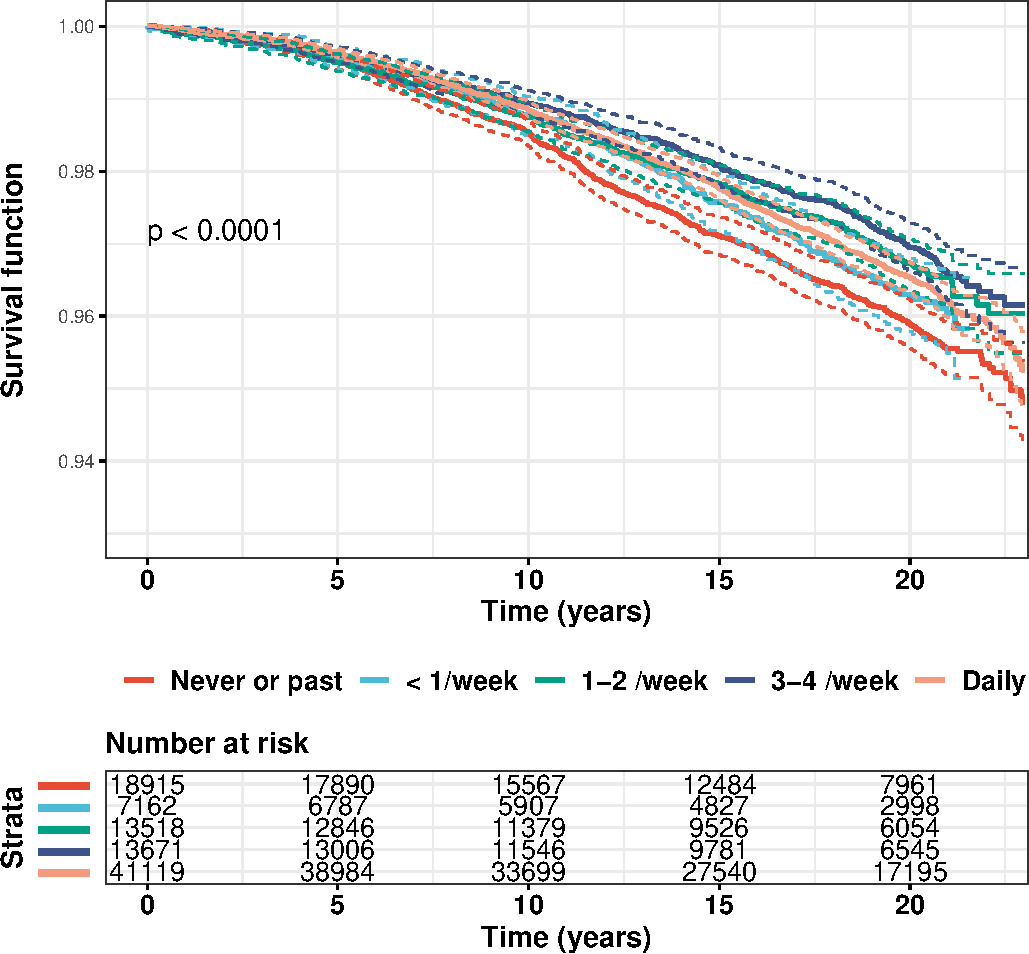
\includegraphics[width=1\linewidth]{traditionalPH_files/figure-latex/fig1-1} 

}

\caption{Kaplan-Meier survival curves for total stroke mortality by drinking frequency (P value was obtained from log-rank tests) in Men.}\label{fig:fig1}
\end{figure}
\begin{figure}

{\centering 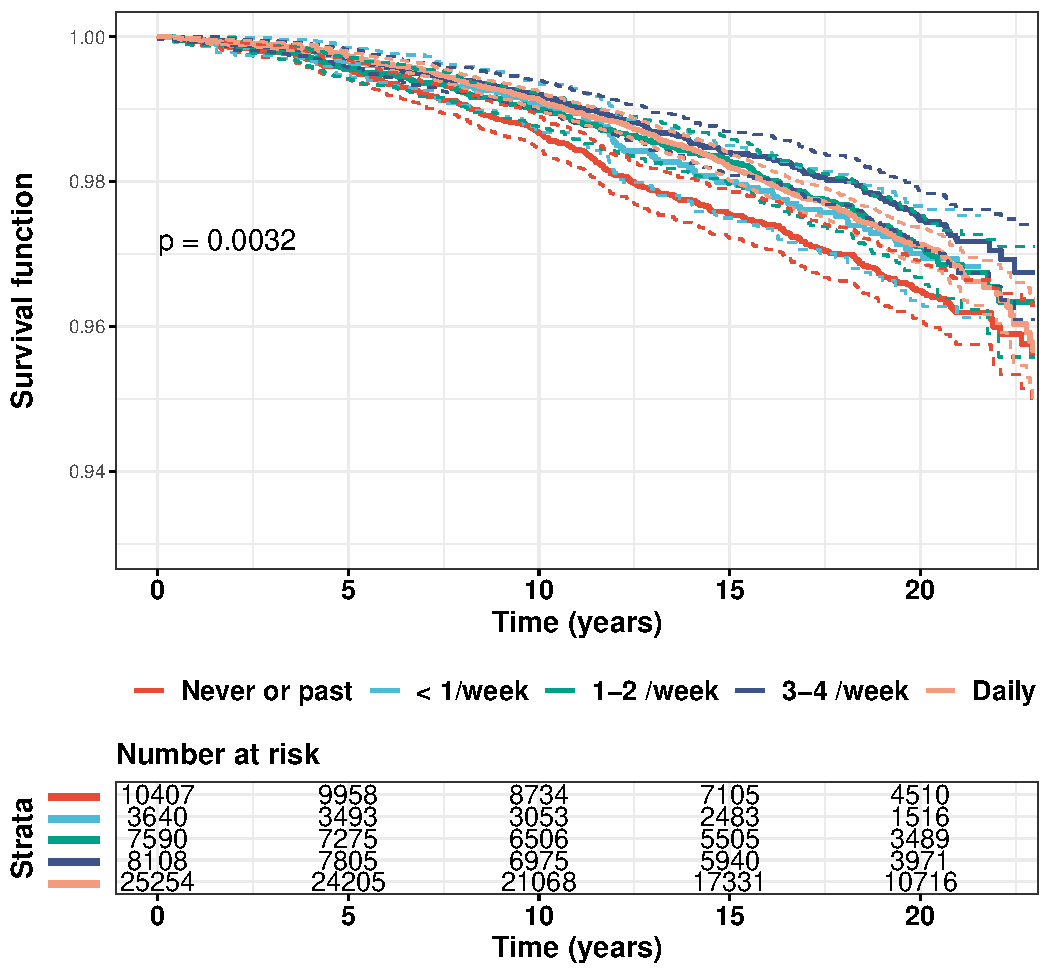
\includegraphics[width=1\linewidth]{traditionalPH_files/figure-latex/fig2-1} 

}

\caption{Kaplan-Meier survival curves for total stroke mortality by drinking frequency (P value was obtained from log-rank tests) in Women.}\label{fig:fig2}
\end{figure}

\hypertarget{in-men}{%
\section{In Men}\label{in-men}}

\hypertarget{model0}{%
\subsection{Model0}\label{model0}}

\begin{Shaded}
\begin{Highlighting}[]
\NormalTok{SurvM0 <-}\StringTok{  }\KeywordTok{coxph}\NormalTok{(su_obj_men }\OperatorTok{~}\StringTok{ }\NormalTok{Mlkfre, }
                 \DataTypeTok{data =}\NormalTok{ MData_men)}

\KeywordTok{library}\NormalTok{(}\StringTok{"broom"}\NormalTok{)}
\KeywordTok{tidy}\NormalTok{(SurvM0, }\DataTypeTok{exponentiate =} \OtherTok{TRUE}\NormalTok{, }\DataTypeTok{conf.int =} \OtherTok{TRUE}\NormalTok{) }\OperatorTok\StringTok{ }
\StringTok{  }\NormalTok{knitr}\OperatorTok{::}\KeywordTok{kable}\NormalTok{(.)}
\end{Highlighting}
\end{Shaded}

\begin{longtable}[]{@{}lrrrrrr@{}}
\toprule
term & estimate & std.error & statistic & p.value & conf.low &
conf.high\tabularnewline
\midrule
\endhead
MlkfreMon1\_2 & 0.8980399 & 0.1061906 & -1.012715 & 0.3111962 &
0.7292997 & 1.1058219\tabularnewline
MlkfreWek1\_2 & 0.7703381 & 0.0927036 & -2.814622 & 0.0048835 &
0.6423503 & 0.9238275\tabularnewline
MlkfreWek3\_4 & 0.7889043 & 0.0933746 & -2.539345 & 0.0111060 &
0.6569672 & 0.9473379\tabularnewline
MlkfreDaily & 0.9024874 & 0.0700243 & -1.465214 & 0.1428626 & 0.7867494
& 1.0352516\tabularnewline
\bottomrule
\end{longtable}

\hypertarget{model1}{%
\subsection{Model1}\label{model1}}

\begin{Shaded}
\begin{Highlighting}[]
\NormalTok{SurvM1 <-}\StringTok{  }\KeywordTok{coxph}\NormalTok{(su_obj_men }\OperatorTok{~}\StringTok{ }\NormalTok{Mlkfre }\OperatorTok{+}\StringTok{ }\NormalTok{Age }\OperatorTok{+}\StringTok{ }\KeywordTok{strata}\NormalTok{(Agegrp), }
                 \DataTypeTok{data =}\NormalTok{ MData_men)}

\KeywordTok{tidy}\NormalTok{(SurvM1, }\DataTypeTok{exponentiate =} \OtherTok{TRUE}\NormalTok{, }\DataTypeTok{conf.int =} \OtherTok{TRUE}\NormalTok{) }\OperatorTok\StringTok{ }
\StringTok{  }\NormalTok{knitr}\OperatorTok{::}\KeywordTok{kable}\NormalTok{(.)}
\end{Highlighting}
\end{Shaded}

\begin{longtable}[]{@{}lrrrrrr@{}}
\toprule
term & estimate & std.error & statistic & p.value & conf.low &
conf.high\tabularnewline
\midrule
\endhead
MlkfreMon1\_2 & 0.9907616 & 0.1062427 & -0.0873596 & 0.9303857 &
0.8045169 & 1.220122\tabularnewline
MlkfreWek1\_2 & 0.8409711 & 0.0927365 & -1.8676357 & 0.0618129 &
0.7012029 & 1.008599\tabularnewline
MlkfreWek3\_4 & 0.8601705 & 0.0934625 & -1.6116056 & 0.1070478 &
0.7161915 & 1.033094\tabularnewline
MlkfreDaily & 0.7599266 & 0.0701965 & -3.9109300 & 0.0000919 & 0.6622475
& 0.872013\tabularnewline
Age & 1.1459568 & 0.0104664 & 13.0169169 & 0.0000000 & 1.1226884 &
1.169707\tabularnewline
\bottomrule
\end{longtable}

\hypertarget{model2}{%
\subsection{Model2}\label{model2}}

\begin{Shaded}
\begin{Highlighting}[]
\NormalTok{SurvM2 <-}\StringTok{  }\KeywordTok{coxph}\NormalTok{(su_obj_men }\OperatorTok{~}\StringTok{ }\NormalTok{Mlkfre }\OperatorTok{+}\StringTok{ }\NormalTok{Age }\OperatorTok{+}\StringTok{ }\KeywordTok{strata}\NormalTok{(Agegrp) }\OperatorTok{+}\StringTok{ }\NormalTok{Smoking }\OperatorTok{+}\StringTok{ }\NormalTok{Alc_Fre }\OperatorTok{+}\StringTok{ }
\StringTok{                   }\NormalTok{BMIgrp }\OperatorTok{+}\StringTok{ }\NormalTok{DM_hist }\OperatorTok{+}\StringTok{ }\NormalTok{HT_hist }\OperatorTok{+}\StringTok{ }\NormalTok{KID_hist }\OperatorTok{+}\StringTok{ }\NormalTok{LIV_hist }\OperatorTok{+}\StringTok{ }\NormalTok{Exercise }\OperatorTok{+}\StringTok{ }
\StringTok{                   }\NormalTok{Slepgrp }\OperatorTok{+}\StringTok{ }\NormalTok{Spi }\OperatorTok{+}\StringTok{ }\NormalTok{Fru }\OperatorTok{+}\StringTok{ }\NormalTok{Cofe }\OperatorTok{+}\StringTok{ }\NormalTok{Educgrp }\OperatorTok{+}\StringTok{ }\NormalTok{Gretea, }
                 \DataTypeTok{data =}\NormalTok{ MData_men)}

\KeywordTok{tidy}\NormalTok{(SurvM2, }\DataTypeTok{exponentiate =} \OtherTok{TRUE}\NormalTok{, }\DataTypeTok{conf.int =} \OtherTok{TRUE}\NormalTok{) }\OperatorTok\StringTok{ }
\StringTok{  }\NormalTok{knitr}\OperatorTok{::}\KeywordTok{kable}\NormalTok{(.)}
\end{Highlighting}
\end{Shaded}

\begin{longtable}[]{@{}lrrrrrr@{}}
\toprule
term & estimate & std.error & statistic & p.value & conf.low &
conf.high\tabularnewline
\midrule
\endhead
MlkfreMon1\_2 & 1.0300683 & 0.1075649 & 0.2754162 & 0.7829965 &
0.8342700 & 1.2718194\tabularnewline
MlkfreWek1\_2 & 0.9061404 & 0.0938429 & -1.0502765 & 0.2935910 &
0.7539044 & 1.0891175\tabularnewline
MlkfreWek3\_4 & 0.9628179 & 0.0951889 & -0.3980606 & 0.6905855 &
0.7989493 & 1.1602968\tabularnewline
MlkfreDaily & 0.8734559 & 0.0730451 & -1.8522475 & 0.0639903 & 0.7569459
& 1.0078992\tabularnewline
Age & 1.1384612 & 0.0105716 & 12.2666081 & 0.0000000 & 1.1151151 &
1.1622961\tabularnewline
SmokingPast & 0.9092779 & 0.0846937 & -1.1229241 & 0.2614697 & 0.7702031
& 1.0734652\tabularnewline
SmokingCurrent & 1.3075884 & 0.0753798 & 3.5577787 & 0.0003740 &
1.1279963 & 1.5157739\tabularnewline
Smokingunknown & 1.2149551 & 0.1306811 & 1.4899405 & 0.1362399 &
0.9404252 & 1.5696260\tabularnewline
Alc\_Fre1-4 /week & 1.1712398 & 0.1770038 & 0.8929911 & 0.3718620 &
0.8279038 & 1.6569590\tabularnewline
Alc\_FreDaily & 1.2876971 & 0.1642444 & 1.5395075 & 0.1236805 &
0.9332729 & 1.7767191\tabularnewline
Alc\_FreNever or past & 1.3967678 & 0.1675560 & 1.9943231 & 0.0461168 &
1.0057737 & 1.9397606\tabularnewline
Alc\_Freunknown & 1.6472841 & 0.1845000 & 2.7053004 & 0.0068243 &
1.1474184 & 2.3649131\tabularnewline
BMIgrp{[}14,18.5) & 1.5003884 & 0.0987751 & 4.1075518 & 0.0000400 &
1.2363065 & 1.8208797\tabularnewline
BMIgrp{[}25,30) & 1.0203389 & 0.0796094 & 0.2529201 & 0.8003300 &
0.8729328 & 1.1926365\tabularnewline
BMIgrp{[}30,40) & 1.4492199 & 0.2612867 & 1.4199934 & 0.1556096 &
0.8684136 & 2.4184769\tabularnewline
BMIgrpunknown & 1.3817305 & 0.1085374 & 2.9790350 & 0.0028916 &
1.1169562 & 1.7092694\tabularnewline
DM\_histTRUE & 1.2836228 & 0.1041754 & 2.3967887 & 0.0165395 & 1.0465577
& 1.5743877\tabularnewline
DM\_histunknown & 0.7349120 & 0.2150330 & -1.4323589 & 0.1520411 &
0.4821686 & 1.1201387\tabularnewline
HT\_histTRUE & 2.0048982 & 0.0628471 & 11.0680261 & 0.0000000 &
1.7725430 & 2.2677119\tabularnewline
HT\_histunknown & 1.0581766 & 0.1591741 & 0.3552542 & 0.7223992 &
0.7745848 & 1.4455975\tabularnewline
KID\_histTRUE & 1.0042507 & 0.1555771 & 0.0272641 & 0.9782491 &
0.7403118 & 1.3622900\tabularnewline
KID\_histunknown & 1.1556749 & 0.1431050 & 1.0110374 & 0.3119985 &
0.8730206 & 1.5298430\tabularnewline
LIV\_histunknown & 1.0081198 & 0.2277189 & 0.0355131 & 0.9716706 &
0.6451749 & 1.5752402\tabularnewline
Exercise\textgreater{} 1h/w & 0.8888327 & 0.0664392 & -1.7737445 &
0.0761054 & 0.7803094 & 1.0124491\tabularnewline
Exerciseunknown & 0.9479967 & 0.1093089 & -0.4885629 & 0.6251512 &
0.7651787 & 1.1744938\tabularnewline
Slepgrp{[}6.9,7.9) & 1.0683517 & 0.0924097 & 0.7154764 & 0.4743147 &
0.8913637 & 1.2804821\tabularnewline
Slepgrp{[}7.9,8.9) & 1.1667996 & 0.0865878 & 1.7815987 & 0.0748147 &
0.9846744 & 1.3826107\tabularnewline
Slepgrp{[}8.9,23) & 1.4173737 & 0.0980271 & 3.5582586 & 0.0003733 &
1.1696167 & 1.7176123\tabularnewline
Slepgrpunknown & 1.1695862 & 0.1490160 & 1.0512293 & 0.2931533 &
0.8733525 & 1.5662999\tabularnewline
SpiOne2tw & 0.8879411 & 0.1100452 & -1.0800099 & 0.2801378 & 0.7156712 &
1.1016783\tabularnewline
SpiThre4tw & 0.8994989 & 0.1109290 & -0.9548220 & 0.3396677 & 0.7237320
& 1.1179530\tabularnewline
Spidaily & 0.8884849 & 0.1098092 & -1.0767551 & 0.2815897 & 0.7164408 &
1.1018432\tabularnewline
Spiunknown & 0.7855355 & 0.1538560 & -1.5689320 & 0.1166638 & 0.5810364
& 1.0620092\tabularnewline
FruOne2tw & 0.9576372 & 0.0915918 & -0.4725999 & 0.6364986 & 0.8002726 &
1.1459458\tabularnewline
FruThre4tw & 0.9459066 & 0.0960788 & -0.5788107 & 0.5627169 & 0.7835485
& 1.1419068\tabularnewline
Frudaily & 0.8564286 & 0.0973184 & -1.5925488 & 0.1112614 & 0.7077072 &
1.0364032\tabularnewline
Fruunknown & 0.8454586 & 0.1084428 & -1.5480618 & 0.1216074 & 0.6835743
& 1.0456804\tabularnewline
CofeThre3tw & 0.9710044 & 0.0723145 & -0.4068925 & 0.6840869 & 0.8426884
& 1.1188592\tabularnewline
CofeNever & 1.1891236 & 0.0703079 & 2.4636845 & 0.0137517 & 1.0360501 &
1.3648132\tabularnewline
Cofeunknown & 1.3526782 & 0.1679593 & 1.7985693 & 0.0720868 & 0.9732564
& 1.8800169\tabularnewline
Educgrp{[}18,70) & 0.8185838 & 0.0738148 & -2.7119167 & 0.0066895 &
0.7083239 & 0.9460071\tabularnewline
Educgrpunknown & 1.0186215 & 0.0801000 & 0.2303397 & 0.8178278 &
0.8706259 & 1.1917744\tabularnewline
GreteaThre3tw & 0.9018289 & 0.1051730 & -0.9824806 & 0.3258631 &
0.7338389 & 1.1082751\tabularnewline
GreteaNever & 1.1039716 & 0.1115240 & 0.8869319 & 0.3751155 & 0.8872142
& 1.3736854\tabularnewline
Greteaunknown & 1.0051178 & 0.1238702 & 0.0412106 & 0.9671280 &
0.7884579 & 1.2813136\tabularnewline
\bottomrule
\end{longtable}

\hypertarget{in-women}{%
\section{In women}\label{in-women}}

\hypertarget{model0-1}{%
\subsection{Model0}\label{model0-1}}

\begin{Shaded}
\begin{Highlighting}[]
\NormalTok{SurvM0 <-}\StringTok{  }\KeywordTok{coxph}\NormalTok{(su_obj_fem }\OperatorTok{~}\StringTok{ }\NormalTok{Mlkfre, }
                 \DataTypeTok{data =}\NormalTok{ MData_fem)}

\KeywordTok{library}\NormalTok{(}\StringTok{"broom"}\NormalTok{)}
\KeywordTok{tidy}\NormalTok{(SurvM0, }\DataTypeTok{exponentiate =} \OtherTok{TRUE}\NormalTok{, }\DataTypeTok{conf.int =} \OtherTok{TRUE}\NormalTok{) }\OperatorTok\StringTok{ }
\StringTok{  }\NormalTok{knitr}\OperatorTok{::}\KeywordTok{kable}\NormalTok{(.)}
\end{Highlighting}
\end{Shaded}

\begin{longtable}[]{@{}lrrrrrr@{}}
\toprule
term & estimate & std.error & statistic & p.value & conf.low &
conf.high\tabularnewline
\midrule
\endhead
MlkfreMon1\_2 & 0.8256913 & 0.1235535 & -1.550213 & 0.1210903 &
0.6481100 & 1.0519295\tabularnewline
MlkfreWek1\_2 & 0.8093525 & 0.0939774 & -2.250762 & 0.0244006 &
0.6731998 & 0.9730416\tabularnewline
MlkfreWek3\_4 & 0.6993278 & 0.0956485 & -3.739060 & 0.0001847 &
0.5797819 & 0.8435231\tabularnewline
MlkfreDaily & 0.8126953 & 0.0710695 & -2.918256 & 0.0035199 & 0.7070226
& 0.9341621\tabularnewline
\bottomrule
\end{longtable}

\hypertarget{model1-1}{%
\subsection{Model1}\label{model1-1}}

\begin{Shaded}
\begin{Highlighting}[]
\NormalTok{SurvM1 <-}\StringTok{  }\KeywordTok{coxph}\NormalTok{(su_obj_fem }\OperatorTok{~}\StringTok{ }\NormalTok{Mlkfre }\OperatorTok{+}\StringTok{ }\NormalTok{Age }\OperatorTok{+}\StringTok{ }\KeywordTok{strata}\NormalTok{(Agegrp), }
                 \DataTypeTok{data =}\NormalTok{ MData_fem)}

\KeywordTok{tidy}\NormalTok{(SurvM1, }\DataTypeTok{exponentiate =} \OtherTok{TRUE}\NormalTok{, }\DataTypeTok{conf.int =} \OtherTok{TRUE}\NormalTok{) }\OperatorTok\StringTok{ }
\StringTok{  }\NormalTok{knitr}\OperatorTok{::}\KeywordTok{kable}\NormalTok{(.)}
\end{Highlighting}
\end{Shaded}

\begin{longtable}[]{@{}lrrrrrr@{}}
\toprule
term & estimate & std.error & statistic & p.value & conf.low &
conf.high\tabularnewline
\midrule
\endhead
MlkfreMon1\_2 & 1.0083893 & 0.1236489 & 0.0675651 & 0.9461319 &
0.7913673 & 1.284927\tabularnewline
MlkfreWek1\_2 & 1.0659228 & 0.0941722 & 0.6779174 & 0.4978240 &
0.8862705 & 1.281992\tabularnewline
MlkfreWek3\_4 & 0.9382761 & 0.0959736 & -0.6638386 & 0.5067936 &
0.7773879 & 1.132462\tabularnewline
MlkfreDaily & 0.8805198 & 0.0711912 & -1.7873398 & 0.0738826 & 0.7658453
& 1.012365\tabularnewline
Age & 1.1568656 & 0.0108181 & 13.4695388 & 0.0000000 & 1.1325948 &
1.181657\tabularnewline
\bottomrule
\end{longtable}

\hypertarget{model2-1}{%
\subsection{Model2}\label{model2-1}}

\begin{Shaded}
\begin{Highlighting}[]
\NormalTok{SurvM2 <-}\StringTok{  }\KeywordTok{coxph}\NormalTok{(su_obj_fem }\OperatorTok{~}\StringTok{ }\NormalTok{Mlkfre }\OperatorTok{+}\StringTok{ }\NormalTok{Age }\OperatorTok{+}\StringTok{ }\KeywordTok{strata}\NormalTok{(Agegrp) }\OperatorTok{+}\StringTok{ }\NormalTok{Smoking }\OperatorTok{+}\StringTok{ }\NormalTok{Alc_Fre }\OperatorTok{+}\StringTok{ }
\StringTok{                   }\NormalTok{BMIgrp }\OperatorTok{+}\StringTok{ }\NormalTok{DM_hist }\OperatorTok{+}\StringTok{ }\NormalTok{HT_hist }\OperatorTok{+}\StringTok{ }\NormalTok{KID_hist }\OperatorTok{+}\StringTok{ }\NormalTok{LIV_hist }\OperatorTok{+}\StringTok{ }\NormalTok{Exercise }\OperatorTok{+}\StringTok{ }
\StringTok{                   }\NormalTok{Slepgrp }\OperatorTok{+}\StringTok{ }\NormalTok{Spi }\OperatorTok{+}\StringTok{ }\NormalTok{Fru }\OperatorTok{+}\StringTok{ }\NormalTok{Cofe }\OperatorTok{+}\StringTok{ }\NormalTok{Educgrp }\OperatorTok{+}\StringTok{ }\NormalTok{Gretea }\OperatorTok{+}\StringTok{ }\NormalTok{Menopause, }
                 \DataTypeTok{data =}\NormalTok{ MData_fem)}

\KeywordTok{tidy}\NormalTok{(SurvM2, }\DataTypeTok{exponentiate =} \OtherTok{TRUE}\NormalTok{, }\DataTypeTok{conf.int =} \OtherTok{TRUE}\NormalTok{) }\OperatorTok\StringTok{ }
\StringTok{  }\NormalTok{knitr}\OperatorTok{::}\KeywordTok{kable}\NormalTok{(.)}
\end{Highlighting}
\end{Shaded}

\begin{longtable}[]{@{}lrrrrrr@{}}
\toprule
term & estimate & std.error & statistic & p.value & conf.low &
conf.high\tabularnewline
\midrule
\endhead
MlkfreMon1\_2 & 1.0467014 & 0.1247926 & 0.3657564 & 0.7145468 &
0.8195947 & 1.3367387\tabularnewline
MlkfreWek1\_2 & 1.1201783 & 0.0952611 & 1.1913348 & 0.2335222 &
0.9293959 & 1.3501238\tabularnewline
MlkfreWek3\_4 & 1.0102846 & 0.0975905 & 0.1048466 & 0.9164975 &
0.8344005 & 1.2232434\tabularnewline
MlkfreDaily & 0.9996588 & 0.0738354 & -0.0046219 & 0.9963123 & 0.8649738
& 1.1553156\tabularnewline
Age & 1.1482663 & 0.0112234 & 12.3182668 & 0.0000000 & 1.1232831 &
1.1738052\tabularnewline
SmokingPast & 0.7785600 & 0.2331089 & -1.0737866 & 0.2829183 & 0.4930256
& 1.2294609\tabularnewline
SmokingCurrent & 1.3300166 & 0.1234733 & 2.3097412 & 0.0209025 &
1.0441343 & 1.6941729\tabularnewline
Smokingunknown & 0.9301666 & 0.0997157 & -0.7259793 & 0.4678515 &
0.7650372 & 1.1309384\tabularnewline
Alc\_Fre1-4 /week & 0.9838100 & 0.1772855 & -0.0920691 & 0.9266431 &
0.6950332 & 1.3925696\tabularnewline
Alc\_FreDaily & 1.2608056 & 0.1939271 & 1.1950413 & 0.2320709 &
0.8621386 & 1.8438228\tabularnewline
Alc\_FreNever or past & 1.0905128 & 0.1441253 & 0.6011990 & 0.5477074 &
0.8221500 & 1.4464735\tabularnewline
Alc\_Freunknown & 1.3451436 & 0.1659978 & 1.7861726 & 0.0740713 &
0.9715632 & 1.8623713\tabularnewline
BMIgrp{[}14,18.5) & 1.9440536 & 0.0925427 & 7.1834450 & 0.0000000 &
1.6215702 & 2.3306697\tabularnewline
BMIgrp{[}25,30) & 1.1836198 & 0.0732828 & 2.3003690 & 0.0214273 &
1.0252596 & 1.3664402\tabularnewline
BMIgrp{[}30,40) & 1.4915614 & 0.1704111 & 2.3462295 & 0.0189644 &
1.0680386 & 2.0830290\tabularnewline
BMIgrpunknown & 1.5499423 & 0.0883179 & 4.9618198 & 0.0000007 &
1.3035844 & 1.8428582\tabularnewline
DM\_histTRUE & 1.6029204 & 0.1191602 & 3.9596053 & 0.0000751 & 1.2690614
& 2.0246094\tabularnewline
DM\_histunknown & 0.9933242 & 0.2062258 & -0.0324798 & 0.9740895 &
0.6630577 & 1.4880953\tabularnewline
HT\_histTRUE & 1.8212939 & 0.0630436 & 9.5100368 & 0.0000000 & 1.6095972
& 2.0608333\tabularnewline
HT\_histunknown & 1.1165935 & 0.1459095 & 0.7558288 & 0.4497518 &
0.8388741 & 1.4862555\tabularnewline
KID\_histTRUE & 1.1308567 & 0.1408644 & 0.8730064 & 0.3826596 &
0.8580322 & 1.4904300\tabularnewline
KID\_histunknown & 1.1944264 & 0.1396201 & 1.2724967 & 0.2031967 &
0.9084783 & 1.5703781\tabularnewline
LIV\_histunknown & 0.9199420 & 0.2180255 & -0.3827288 & 0.7019208 &
0.6000353 & 1.4104059\tabularnewline
Exercise\textgreater{} 1h/w & 0.9641530 & 0.0724144 & -0.5041158 &
0.6141800 & 0.8365785 & 1.1111821\tabularnewline
Exerciseunknown & 1.0288033 & 0.0967990 & 0.2933536 & 0.7692519 &
0.8510145 & 1.2437348\tabularnewline
Slepgrp{[}6.9,7.9) & 0.9437620 & 0.0820239 & -0.7056632 & 0.4803976 &
0.8036068 & 1.1083613\tabularnewline
Slepgrp{[}7.9,8.9) & 1.1877371 & 0.0764556 & 2.2503248 & 0.0244283 &
1.0224480 & 1.3797469\tabularnewline
Slepgrp{[}8.9,23) & 1.3200220 & 0.0954417 & 2.9090893 & 0.0036248 &
1.0948158 & 1.5915536\tabularnewline
Slepgrpunknown & 1.0404227 & 0.1341486 & 0.2953970 & 0.7676906 &
0.7998754 & 1.3533100\tabularnewline
SpiOne2tw & 0.7553060 & 0.1221389 & -2.2976488 & 0.0215818 & 0.5945085 &
0.9595945\tabularnewline
SpiThre4tw & 0.8809776 & 0.1194692 & -1.0607171 & 0.2888185 & 0.6970637
& 1.1134155\tabularnewline
Spidaily & 0.7782482 & 0.1192466 & -2.1024487 & 0.0355140 & 0.6160490 &
0.9831527\tabularnewline
Spiunknown & 0.7500660 & 0.1561738 & -1.8414993 & 0.0655484 & 0.5522861
& 1.0186733\tabularnewline
FruOne2tw & 0.9005071 & 0.1072566 & -0.9770699 & 0.3285345 & 0.7297769 &
1.1111793\tabularnewline
FruThre4tw & 0.8506338 & 0.1055080 & -1.5332822 & 0.1252063 & 0.6917258
& 1.0460471\tabularnewline
Frudaily & 0.7375555 & 0.1016921 & -2.9934854 & 0.0027581 & 0.6042745 &
0.9002336\tabularnewline
Fruunknown & 0.5994110 & 0.1191553 & -4.2952989 & 0.0000174 & 0.4745692
& 0.7570942\tabularnewline
CofeThre3tw & 0.8460922 & 0.0775884 & -2.1540193 & 0.0312387 & 0.7267321
& 0.9850563\tabularnewline
CofeNever & 1.0163001 & 0.0683542 & 0.2365420 & 0.8130121 & 0.8888711 &
1.1619973\tabularnewline
Cofeunknown & 1.0491755 & 0.1659541 & 0.2892643 & 0.7723791 & 0.7578578
& 1.4524745\tabularnewline
Educgrp{[}18,70) & 0.7838786 & 0.0857662 & -2.8391273 & 0.0045237 &
0.6625894 & 0.9273702\tabularnewline
Educgrpunknown & 1.1213011 & 0.0756084 & 1.5142454 & 0.1299636 &
0.9668614 & 1.3004099\tabularnewline
GreteaThre3tw & 0.9216585 & 0.1045395 & -0.7803800 & 0.4351672 &
0.7509065 & 1.1312386\tabularnewline
GreteaNever & 1.0261198 & 0.1080096 & 0.2387238 & 0.8113197 & 0.8303479
& 1.2680489\tabularnewline
Greteaunknown & 0.9870257 & 0.1183219 & -0.1103701 & 0.9121159 &
0.7827313 & 1.2446414\tabularnewline
MenopauseTRUE & 0.5377835 & 0.2169379 & -2.8593407 & 0.0042452 &
0.3515197 & 0.8227451\tabularnewline
\bottomrule
\end{longtable}

\hypertarget{cause-specific-hemostroke}{%
\section{Cause specific: HemoStroke}\label{cause-specific-hemostroke}}

\begin{Shaded}
\begin{Highlighting}[]
\CommentTok{# in Men}
\NormalTok{su_obj_men <-}\StringTok{ }\KeywordTok{Surv}\NormalTok{(MData_men}\OperatorTok{$}\NormalTok{followpy, MData_men}\OperatorTok{$}\NormalTok{HemoStroke }\OperatorTok{==}\StringTok{ "I60_2"}\NormalTok{)}
\CommentTok{# in Women}
\NormalTok{su_obj_fem <-}\StringTok{ }\KeywordTok{Surv}\NormalTok{(MData_fem}\OperatorTok{$}\NormalTok{followpy, MData_fem}\OperatorTok{$}\NormalTok{HemoStroke }\OperatorTok{==}\StringTok{ "I60_2"}\NormalTok{)}
\end{Highlighting}
\end{Shaded}

\hypertarget{in-men-1}{%
\section{In Men}\label{in-men-1}}

\hypertarget{model0-2}{%
\subsection{Model0}\label{model0-2}}

\begin{Shaded}
\begin{Highlighting}[]
\NormalTok{SurvM0 <-}\StringTok{  }\KeywordTok{coxph}\NormalTok{(su_obj_men }\OperatorTok{~}\StringTok{ }\NormalTok{Mlkfre, }
                 \DataTypeTok{data =}\NormalTok{ MData_men)}

\KeywordTok{library}\NormalTok{(}\StringTok{"broom"}\NormalTok{)}
\KeywordTok{tidy}\NormalTok{(SurvM0, }\DataTypeTok{exponentiate =} \OtherTok{TRUE}\NormalTok{, }\DataTypeTok{conf.int =} \OtherTok{TRUE}\NormalTok{) }\OperatorTok\StringTok{ }
\StringTok{  }\NormalTok{knitr}\OperatorTok{::}\KeywordTok{kable}\NormalTok{(.)}
\end{Highlighting}
\end{Shaded}

\begin{longtable}[]{@{}lrrrrrr@{}}
\toprule
term & estimate & std.error & statistic & p.value & conf.low &
conf.high\tabularnewline
\midrule
\endhead
MlkfreMon1\_2 & 1.0018664 & 0.1839174 & 0.0101387 & 0.9919107 &
0.6986490 & 1.436682\tabularnewline
MlkfreWek1\_2 & 0.8063903 & 0.1650585 & -1.3037040 & 0.1923345 &
0.5835085 & 1.114406\tabularnewline
MlkfreWek3\_4 & 0.8187506 & 0.1669198 & -1.1980353 & 0.2309033 &
0.5902952 & 1.135622\tabularnewline
MlkfreDaily & 0.9442372 & 0.1252492 & -0.4581096 & 0.6468737 & 0.7387012
& 1.206962\tabularnewline
\bottomrule
\end{longtable}

\hypertarget{model1-2}{%
\subsection{Model1}\label{model1-2}}

\begin{Shaded}
\begin{Highlighting}[]
\NormalTok{SurvM1 <-}\StringTok{  }\KeywordTok{coxph}\NormalTok{(su_obj_men }\OperatorTok{~}\StringTok{ }\NormalTok{Mlkfre }\OperatorTok{+}\StringTok{ }\NormalTok{Age }\OperatorTok{+}\StringTok{ }\KeywordTok{strata}\NormalTok{(Agegrp), }
                 \DataTypeTok{data =}\NormalTok{ MData_men)}

\KeywordTok{tidy}\NormalTok{(SurvM1, }\DataTypeTok{exponentiate =} \OtherTok{TRUE}\NormalTok{, }\DataTypeTok{conf.int =} \OtherTok{TRUE}\NormalTok{) }\OperatorTok\StringTok{ }
\StringTok{  }\NormalTok{knitr}\OperatorTok{::}\KeywordTok{kable}\NormalTok{(.)}
\end{Highlighting}
\end{Shaded}

\begin{longtable}[]{@{}lrrrrrr@{}}
\toprule
term & estimate & std.error & statistic & p.value & conf.low &
conf.high\tabularnewline
\midrule
\endhead
MlkfreMon1\_2 & 1.0771740 & 0.1840374 & 0.4039446 & 0.6862535 &
0.7509878 & 1.545037\tabularnewline
MlkfreWek1\_2 & 0.8593591 & 0.1651432 & -0.9178000 & 0.3587236 &
0.6217338 & 1.187804\tabularnewline
MlkfreWek3\_4 & 0.8703379 & 0.1670434 & -0.8313635 & 0.4057683 &
0.6273362 & 1.207467\tabularnewline
MlkfreDaily & 0.8463106 & 0.1255224 & -1.3293948 & 0.1837177 & 0.6617361
& 1.082367\tabularnewline
Age & 1.0812843 & 0.0183013 & 4.2701629 & 0.0000195 & 1.0431862 &
1.120774\tabularnewline
\bottomrule
\end{longtable}

\hypertarget{model2-2}{%
\subsection{Model2}\label{model2-2}}

\begin{Shaded}
\begin{Highlighting}[]
\NormalTok{SurvM2 <-}\StringTok{  }\KeywordTok{coxph}\NormalTok{(su_obj_men }\OperatorTok{~}\StringTok{ }\NormalTok{Mlkfre }\OperatorTok{+}\StringTok{ }\NormalTok{Age }\OperatorTok{+}\StringTok{ }\KeywordTok{strata}\NormalTok{(Agegrp) }\OperatorTok{+}\StringTok{ }\NormalTok{Smoking }\OperatorTok{+}\StringTok{ }\NormalTok{Alc_Fre }\OperatorTok{+}\StringTok{ }
\StringTok{                   }\NormalTok{BMIgrp }\OperatorTok{+}\StringTok{ }\NormalTok{DM_hist }\OperatorTok{+}\StringTok{ }\NormalTok{HT_hist }\OperatorTok{+}\StringTok{ }\NormalTok{KID_hist }\OperatorTok{+}\StringTok{ }\NormalTok{LIV_hist }\OperatorTok{+}\StringTok{ }\NormalTok{Exercise }\OperatorTok{+}\StringTok{ }
\StringTok{                   }\NormalTok{Slepgrp }\OperatorTok{+}\StringTok{ }\NormalTok{Spi }\OperatorTok{+}\StringTok{ }\NormalTok{Fru }\OperatorTok{+}\StringTok{ }\NormalTok{Cofe }\OperatorTok{+}\StringTok{ }\NormalTok{Educgrp }\OperatorTok{+}\StringTok{ }\NormalTok{Gretea, }
                 \DataTypeTok{data =}\NormalTok{ MData_men)}

\KeywordTok{tidy}\NormalTok{(SurvM2, }\DataTypeTok{exponentiate =} \OtherTok{TRUE}\NormalTok{, }\DataTypeTok{conf.int =} \OtherTok{TRUE}\NormalTok{) }\OperatorTok\StringTok{ }
\StringTok{  }\NormalTok{knitr}\OperatorTok{::}\KeywordTok{kable}\NormalTok{(.)}
\end{Highlighting}
\end{Shaded}

\begin{longtable}[]{@{}lrrrrrr@{}}
\toprule
term & estimate & std.error & statistic & p.value & conf.low &
conf.high\tabularnewline
\midrule
\endhead
MlkfreMon1\_2 & 1.1134015 & 0.1861324 & 0.5771147 & 0.5638619 &
0.7730643 & 1.6035704\tabularnewline
MlkfreWek1\_2 & 0.9449402 & 0.1668809 & -0.3393658 & 0.7343342 &
0.6813261 & 1.3105499\tabularnewline
MlkfreWek3\_4 & 1.0062269 & 0.1696694 & 0.0365865 & 0.9708147 &
0.7215611 & 1.4031973\tabularnewline
MlkfreDaily & 0.9832157 & 0.1301855 & -0.1300206 & 0.8965502 & 0.7617890
& 1.2690037\tabularnewline
Age & 1.0777785 & 0.0185111 & 4.0463314 & 0.0000520 & 1.0393764 &
1.1175995\tabularnewline
SmokingPast & 1.0101500 & 0.1598623 & 0.0631722 & 0.9496294 & 0.7384326
& 1.3818499\tabularnewline
SmokingCurrent & 1.5772291 & 0.1394669 & 3.2672238 & 0.0010861 &
1.1999975 & 2.0730474\tabularnewline
Smokingunknown & 1.1449340 & 0.2614826 & 0.5176138 & 0.6047277 &
0.6858136 & 1.9114143\tabularnewline
Alc\_Fre1-4 /week & 1.2141812 & 0.3086607 & 0.6287483 & 0.5295139 &
0.6630572 & 2.2233918\tabularnewline
Alc\_FreDaily & 1.3914300 & 0.2870213 & 1.1508970 & 0.2497746 &
0.7927721 & 2.4421613\tabularnewline
Alc\_FreNever or past & 1.1796936 & 0.2978239 & 0.5548738 & 0.5789810 &
0.6580532 & 2.1148395\tabularnewline
Alc\_Freunknown & 1.8929475 & 0.3238383 & 1.9705362 & 0.0487770 &
1.0034295 & 3.5710035\tabularnewline
BMIgrp{[}14,18.5) & 1.6674550 & 0.1753523 & 2.9158352 & 0.0035474 &
1.1824804 & 2.3513338\tabularnewline
BMIgrp{[}25,30) & 0.9304614 & 0.1420159 & -0.5075113 & 0.6117961 &
0.7043917 & 1.2290867\tabularnewline
BMIgrp{[}30,40) & 0.8207613 & 0.5813293 & -0.3397780 & 0.7340237 &
0.2626567 & 2.5647515\tabularnewline
BMIgrpunknown & 1.5642777 & 0.1952663 & 2.2913544 & 0.0219429 &
1.0668489 & 2.2936376\tabularnewline
DM\_histTRUE & 1.1481046 & 0.1948149 & 0.7089417 & 0.4783606 & 0.7837088
& 1.6819311\tabularnewline
DM\_histunknown & 0.6113172 & 0.3780974 & -1.3016203 & 0.1930462 &
0.2913598 & 1.2826369\tabularnewline
HT\_histTRUE & 1.7780869 & 0.1152353 & 4.9944612 & 0.0000006 & 1.4186150
& 2.2286477\tabularnewline
HT\_histunknown & 0.8823975 & 0.2928417 & -0.4272363 & 0.6692072 &
0.4970465 & 1.5665043\tabularnewline
KID\_histTRUE & 1.3996573 & 0.2392006 & 1.4056296 & 0.1598342 &
0.8758179 & 2.2368129\tabularnewline
KID\_histunknown & 1.2380224 & 0.2572768 & 0.8299050 & 0.4065925 &
0.7477116 & 2.0498538\tabularnewline
LIV\_histunknown & 1.2593850 & 0.3985347 & 0.5786785 & 0.5628061 &
0.5766670 & 2.7503749\tabularnewline
Exercise\textgreater{} 1h/w & 0.9682060 & 0.1153437 & -0.2801232 &
0.7793830 & 0.7723018 & 1.2138037\tabularnewline
Exerciseunknown & 0.5319369 & 0.2352731 & -2.6829691 & 0.0072972 &
0.3354249 & 0.8435774\tabularnewline
Slepgrp{[}6.9,7.9) & 0.8611806 & 0.1514075 & -0.9870778 & 0.3236045 &
0.6400530 & 1.1587042\tabularnewline
Slepgrp{[}7.9,8.9) & 0.9822738 & 0.1415537 & -0.1263490 & 0.8994557 &
0.7442894 & 1.2963531\tabularnewline
Slepgrp{[}8.9,23) & 0.9775126 & 0.1757417 & -0.1294178 & 0.8970271 &
0.6926771 & 1.3794753\tabularnewline
Slepgrpunknown & 0.9215609 & 0.2753945 & -0.2966160 & 0.7667597 &
0.5371651 & 1.5810306\tabularnewline
SpiOne2tw & 0.8537835 & 0.1781728 & -0.8872149 & 0.3749632 & 0.6021252 &
1.2106226\tabularnewline
SpiThre4tw & 0.7694934 & 0.1846042 & -1.4193772 & 0.1557891 & 0.5358824
& 1.1049439\tabularnewline
Spidaily & 0.7515458 & 0.1839380 & -1.5528232 & 0.1204654 & 0.5240674 &
1.0777641\tabularnewline
Spiunknown & 0.9478997 & 0.2727461 & -0.1961771 & 0.8444715 & 0.5553932
& 1.6177979\tabularnewline
FruOne2tw & 0.8904068 & 0.1547156 & -0.7502593 & 0.4530985 & 0.6574977 &
1.2058205\tabularnewline
FruThre4tw & 0.7911651 & 0.1687246 & -1.3883487 & 0.1650309 & 0.5683927
& 1.1012496\tabularnewline
Frudaily & 0.8317243 & 0.1667143 & -1.1052102 & 0.2690685 & 0.5998905 &
1.1531527\tabularnewline
Fruunknown & 0.9440623 & 0.1871852 & -0.3075197 & 0.7584478 & 0.6541364
& 1.3624888\tabularnewline
CofeThre3tw & 1.0381434 & 0.1283458 & 0.2916649 & 0.7705429 & 0.8072522
& 1.3350745\tabularnewline
CofeNever & 1.3908326 & 0.1239529 & 2.6615152 & 0.0077790 & 1.0908523 &
1.7733064\tabularnewline
Cofeunknown & 1.1266999 & 0.3206563 & 0.3720275 & 0.7098724 & 0.6009871
& 2.1122796\tabularnewline
Educgrp{[}18,70) & 0.9415033 & 0.1223844 & -0.4925254 & 0.6223480 &
0.7407098 & 1.1967284\tabularnewline
Educgrpunknown & 0.8634590 & 0.1515303 & -0.9688417 & 0.3326242 &
0.6415919 & 1.1620493\tabularnewline
GreteaThre3tw & 0.7235100 & 0.2050131 & -1.5786357 & 0.1144196 &
0.4841022 & 1.0813143\tabularnewline
GreteaNever & 1.2481441 & 0.1869247 & 1.1858131 & 0.2356961 & 0.8652750
& 1.8004261\tabularnewline
Greteaunknown & 1.7690641 & 0.1998633 & 2.8542035 & 0.0043145 &
1.1956927 & 2.6173847\tabularnewline
\bottomrule
\end{longtable}

\hypertarget{in-women-1}{%
\section{In women}\label{in-women-1}}

\hypertarget{model0-3}{%
\subsection{Model0}\label{model0-3}}

\begin{Shaded}
\begin{Highlighting}[]
\NormalTok{SurvM0 <-}\StringTok{  }\KeywordTok{coxph}\NormalTok{(su_obj_fem }\OperatorTok{~}\StringTok{ }\NormalTok{Mlkfre, }
                 \DataTypeTok{data =}\NormalTok{ MData_fem)}

\KeywordTok{library}\NormalTok{(}\StringTok{"broom"}\NormalTok{)}
\KeywordTok{tidy}\NormalTok{(SurvM0, }\DataTypeTok{exponentiate =} \OtherTok{TRUE}\NormalTok{, }\DataTypeTok{conf.int =} \OtherTok{TRUE}\NormalTok{) }\OperatorTok\StringTok{ }
\StringTok{  }\NormalTok{knitr}\OperatorTok{::}\KeywordTok{kable}\NormalTok{(.)}
\end{Highlighting}
\end{Shaded}

\begin{longtable}[]{@{}lrrrrrr@{}}
\toprule
term & estimate & std.error & statistic & p.value & conf.low &
conf.high\tabularnewline
\midrule
\endhead
MlkfreMon1\_2 & 0.7329251 & 0.2152953 & -1.4431888 & 0.1489673 &
0.4806178 & 1.117685\tabularnewline
MlkfreWek1\_2 & 0.9656254 & 0.1486205 & -0.2353601 & 0.8139292 &
0.7216103 & 1.292155\tabularnewline
MlkfreWek3\_4 & 0.8631136 & 0.1497347 & -0.9831320 & 0.3255425 &
0.6435964 & 1.157504\tabularnewline
MlkfreDaily & 0.8894565 & 0.1166414 & -1.0043148 & 0.3152269 & 0.7076840
& 1.117918\tabularnewline
\bottomrule
\end{longtable}

\hypertarget{model1-3}{%
\subsection{Model1}\label{model1-3}}

\begin{Shaded}
\begin{Highlighting}[]
\NormalTok{SurvM1 <-}\StringTok{  }\KeywordTok{coxph}\NormalTok{(su_obj_fem }\OperatorTok{~}\StringTok{ }\NormalTok{Mlkfre }\OperatorTok{+}\StringTok{ }\NormalTok{Age }\OperatorTok{+}\StringTok{ }\KeywordTok{strata}\NormalTok{(Agegrp), }
                 \DataTypeTok{data =}\NormalTok{ MData_fem)}

\KeywordTok{tidy}\NormalTok{(SurvM1, }\DataTypeTok{exponentiate =} \OtherTok{TRUE}\NormalTok{, }\DataTypeTok{conf.int =} \OtherTok{TRUE}\NormalTok{) }\OperatorTok\StringTok{ }
\StringTok{  }\NormalTok{knitr}\OperatorTok{::}\KeywordTok{kable}\NormalTok{(.)}
\end{Highlighting}
\end{Shaded}

\begin{longtable}[]{@{}lrrrrrr@{}}
\toprule
term & estimate & std.error & statistic & p.value & conf.low &
conf.high\tabularnewline
\midrule
\endhead
MlkfreMon1\_2 & 0.8288805 & 0.2154022 & -0.8712967 & 0.3835922 &
0.5434271 & 1.264278\tabularnewline
MlkfreWek1\_2 & 1.1565026 & 0.1489302 & 0.9762997 & 0.3289160 &
0.8637281 & 1.548518\tabularnewline
MlkfreWek3\_4 & 1.0356829 & 0.1501549 & 0.2334987 & 0.8153742 &
0.7716399 & 1.390077\tabularnewline
MlkfreDaily & 0.9155020 & 0.1167504 & -0.7561665 & 0.4495494 & 0.7282512
& 1.150899\tabularnewline
Age & 1.0972778 & 0.0164735 & 5.6352378 & 0.0000000 & 1.0624152 &
1.133284\tabularnewline
\bottomrule
\end{longtable}

\hypertarget{model2-3}{%
\subsection{Model2}\label{model2-3}}

\begin{Shaded}
\begin{Highlighting}[]
\NormalTok{SurvM2 <-}\StringTok{  }\KeywordTok{coxph}\NormalTok{(su_obj_fem }\OperatorTok{~}\StringTok{ }\NormalTok{Mlkfre }\OperatorTok{+}\StringTok{ }\NormalTok{Age }\OperatorTok{+}\StringTok{ }\KeywordTok{strata}\NormalTok{(Agegrp) }\OperatorTok{+}\StringTok{ }\NormalTok{Smoking }\OperatorTok{+}\StringTok{ }\NormalTok{Alc_Fre }\OperatorTok{+}\StringTok{ }
\StringTok{                   }\NormalTok{BMIgrp }\OperatorTok{+}\StringTok{ }\NormalTok{DM_hist }\OperatorTok{+}\StringTok{ }\NormalTok{HT_hist }\OperatorTok{+}\StringTok{ }\NormalTok{KID_hist }\OperatorTok{+}\StringTok{ }\NormalTok{LIV_hist }\OperatorTok{+}\StringTok{ }\NormalTok{Exercise }\OperatorTok{+}\StringTok{ }
\StringTok{                   }\NormalTok{Slepgrp }\OperatorTok{+}\StringTok{ }\NormalTok{Spi }\OperatorTok{+}\StringTok{ }\NormalTok{Fru }\OperatorTok{+}\StringTok{ }\NormalTok{Cofe }\OperatorTok{+}\StringTok{ }\NormalTok{Educgrp }\OperatorTok{+}\StringTok{ }\NormalTok{Gretea }\OperatorTok{+}\StringTok{ }\NormalTok{Menopause, }
                 \DataTypeTok{data =}\NormalTok{ MData_fem)}

\KeywordTok{tidy}\NormalTok{(SurvM2, }\DataTypeTok{exponentiate =} \OtherTok{TRUE}\NormalTok{, }\DataTypeTok{conf.int =} \OtherTok{TRUE}\NormalTok{) }\OperatorTok\StringTok{ }
\StringTok{  }\NormalTok{knitr}\OperatorTok{::}\KeywordTok{kable}\NormalTok{(.)}
\end{Highlighting}
\end{Shaded}

\begin{longtable}[]{@{}lrrrrrr@{}}
\toprule
term & estimate & std.error & statistic & p.value & conf.low &
conf.high\tabularnewline
\midrule
\endhead
MlkfreMon1\_2 & 0.8523110 & 0.2168453 & -0.7369484 & 0.4611537 &
0.5572102 & 1.3036985\tabularnewline
MlkfreWek1\_2 & 1.2087347 & 0.1503743 & 1.2606816 & 0.2074236 &
0.9001858 & 1.6230421\tabularnewline
MlkfreWek3\_4 & 1.1301093 & 0.1524809 & 0.8021618 & 0.4224594 &
0.8381630 & 1.5237455\tabularnewline
MlkfreDaily & 1.0258900 & 0.1206184 & 0.2119123 & 0.8321755 & 0.8098978
& 1.2994853\tabularnewline
Age & 1.0863261 & 0.0173859 & 4.7625505 & 0.0000019 & 1.0499322 &
1.1239815\tabularnewline
SmokingPast & 0.6383644 & 0.4517490 & -0.9935739 & 0.3204304 & 0.2633535
& 1.5473841\tabularnewline
SmokingCurrent & 1.8225964 & 0.1723866 & 3.4820703 & 0.0004976 &
1.3000343 & 2.5552077\tabularnewline
Smokingunknown & 0.9851802 & 0.1586694 & -0.0940998 & 0.9250299 &
0.7218651 & 1.3445449\tabularnewline
Alc\_Fre1-4 /week & 0.6640513 & 0.2444429 & -1.6748122 & 0.0939711 &
0.4112742 & 1.0721900\tabularnewline
Alc\_FreDaily & 0.8172757 & 0.2790388 & -0.7231207 & 0.4696057 &
0.4729882 & 1.4121697\tabularnewline
Alc\_FreNever or past & 0.7958204 & 0.1873558 & -1.2189731 & 0.2228544 &
0.5512359 & 1.1489276\tabularnewline
Alc\_Freunknown & 0.9091069 & 0.2317336 & -0.4112163 & 0.6809139 &
0.5772487 & 1.4317491\tabularnewline
BMIgrp{[}14,18.5) & 2.4042129 & 0.1409511 & 6.2235962 & 0.0000000 &
1.8238753 & 3.1692077\tabularnewline
BMIgrp{[}25,30) & 1.0516113 & 0.1164995 & 0.4319636 & 0.6657679 &
0.8369329 & 1.3213560\tabularnewline
BMIgrp{[}30,40) & 0.7820537 & 0.3601086 & -0.6826604 & 0.4948214 &
0.3861105 & 1.5840233\tabularnewline
BMIgrpunknown & 1.6019762 & 0.1528058 & 3.0839007 & 0.0020431 &
1.1873739 & 2.1613475\tabularnewline
DM\_histTRUE & 1.0262080 & 0.2299845 & 0.1124880 & 0.9104365 & 0.6538412
& 1.6106403\tabularnewline
DM\_histunknown & 1.1388221 & 0.3650284 & 0.3561215 & 0.7217496 &
0.5568563 & 2.3289952\tabularnewline
HT\_histTRUE & 2.1598872 & 0.1011615 & 7.6121452 & 0.0000000 & 1.7714229
& 2.6335398\tabularnewline
HT\_histunknown & 0.7796102 & 0.2402212 & -1.0363835 & 0.3000233 &
0.4868564 & 1.2484011\tabularnewline
KID\_histTRUE & 1.2167582 & 0.2142650 & 0.9156424 & 0.3598545 &
0.7995058 & 1.8517696\tabularnewline
KID\_histunknown & 1.0510227 & 0.2292828 & 0.2170407 & 0.8281766 &
0.6705733 & 1.6473199\tabularnewline
LIV\_histunknown & 1.0973036 & 0.3746108 & 0.2478731 & 0.8042326 &
0.5265717 & 2.2866310\tabularnewline
Exercise\textgreater{} 1h/w & 1.1623012 & 0.1122602 & 1.3397608 &
0.1803231 & 0.9327443 & 1.4483541\tabularnewline
Exerciseunknown & 1.2422318 & 0.1541718 & 1.4069341 & 0.1594469 &
0.9182720 & 1.6804823\tabularnewline
Slepgrp{[}6.9,7.9) & 1.0792731 & 0.1228908 & 0.6207768 & 0.5347465 &
0.8482551 & 1.3732076\tabularnewline
Slepgrp{[}7.9,8.9) & 1.1695672 & 0.1222299 & 1.2814687 & 0.2000291 &
0.9204134 & 1.4861663\tabularnewline
Slepgrp{[}8.9,23) & 1.0509384 & 0.1761699 & 0.2820201 & 0.7779281 &
0.7440826 & 1.4843397\tabularnewline
Slepgrpunknown & 1.1683948 & 0.2094594 & 0.7430121 & 0.4574744 &
0.7749924 & 1.7614965\tabularnewline
SpiOne2tw & 0.6798889 & 0.1875493 & -2.0571967 & 0.0396673 & 0.4707558 &
0.9819293\tabularnewline
SpiThre4tw & 0.7479799 & 0.1847923 & -1.5713814 & 0.1160941 & 0.5207083
& 1.0744480\tabularnewline
Spidaily & 0.7965040 & 0.1816674 & -1.2524163 & 0.2104182 & 0.5578949 &
1.1371650\tabularnewline
Spiunknown & 0.6868033 & 0.2467738 & -1.5224763 & 0.1278898 & 0.4234266
& 1.1140037\tabularnewline
FruOne2tw & 1.0772139 & 0.1674429 & 0.4441993 & 0.6568985 & 0.7758439 &
1.4956487\tabularnewline
FruThre4tw & 0.8906245 & 0.1690287 & -0.6852821 & 0.4931659 & 0.6394655
& 1.2404297\tabularnewline
Frudaily & 0.6812614 & 0.1648204 & -2.3286519 & 0.0198775 & 0.4931947 &
0.9410422\tabularnewline
Fruunknown & 0.6735045 & 0.1924663 & -2.0536619 & 0.0400084 & 0.4618627
& 0.9821280\tabularnewline
CofeThre3tw & 0.7964819 & 0.1200031 & -1.8962089 & 0.0579324 & 0.6295483
& 1.0076801\tabularnewline
CofeNever & 0.9900539 & 0.1090474 & -0.0916659 & 0.9269635 & 0.7995350 &
1.2259708\tabularnewline
Cofeunknown & 0.8677467 & 0.3014628 & -0.4705569 & 0.6379572 & 0.4806040
& 1.5667460\tabularnewline
Educgrp{[}18,70) & 0.7404118 & 0.1274145 & -2.3588269 & 0.0183328 &
0.5767903 & 0.9504489\tabularnewline
Educgrpunknown & 0.9351974 & 0.1275887 & -0.5251068 & 0.5995089 &
0.7282821 & 1.2009003\tabularnewline
GreteaThre3tw & 0.8022045 & 0.1688843 & -1.3049866 & 0.1918974 &
0.5761433 & 1.1169652\tabularnewline
GreteaNever & 0.9872543 & 0.1711198 & -0.0749626 & 0.9402445 & 0.7059462
& 1.3806592\tabularnewline
Greteaunknown & 0.7546384 & 0.2126032 & -1.3241404 & 0.1854564 &
0.4974744 & 1.1447407\tabularnewline
MenopauseTRUE & 0.7246684 & 0.2628829 & -1.2250364 & 0.2205615 &
0.4328854 & 1.2131253\tabularnewline
\bottomrule
\end{longtable}

\hypertarget{cause-specific-ischestroke}{%
\section{Cause specific: IscheStroke}\label{cause-specific-ischestroke}}

\begin{Shaded}
\begin{Highlighting}[]
\CommentTok{# in Men}
\NormalTok{su_obj_men <-}\StringTok{ }\KeywordTok{Surv}\NormalTok{(MData_men}\OperatorTok{$}\NormalTok{followpy, MData_men}\OperatorTok{$}\NormalTok{IscheStroke }\OperatorTok{==}\StringTok{ "I63"}\NormalTok{)}
\CommentTok{# in Women}
\NormalTok{su_obj_fem <-}\StringTok{ }\KeywordTok{Surv}\NormalTok{(MData_fem}\OperatorTok{$}\NormalTok{followpy, MData_fem}\OperatorTok{$}\NormalTok{IscheStroke }\OperatorTok{==}\StringTok{ "I63"}\NormalTok{)}
\end{Highlighting}
\end{Shaded}

\hypertarget{in-men-2}{%
\section{In Men}\label{in-men-2}}

\hypertarget{model0-4}{%
\subsection{Model0}\label{model0-4}}

\begin{Shaded}
\begin{Highlighting}[]
\NormalTok{SurvM0 <-}\StringTok{  }\KeywordTok{coxph}\NormalTok{(su_obj_men }\OperatorTok{~}\StringTok{ }\NormalTok{Mlkfre, }
                 \DataTypeTok{data =}\NormalTok{ MData_men)}

\KeywordTok{library}\NormalTok{(}\StringTok{"broom"}\NormalTok{)}
\KeywordTok{tidy}\NormalTok{(SurvM0, }\DataTypeTok{exponentiate =} \OtherTok{TRUE}\NormalTok{, }\DataTypeTok{conf.int =} \OtherTok{TRUE}\NormalTok{) }\OperatorTok\StringTok{ }
\StringTok{  }\NormalTok{knitr}\OperatorTok{::}\KeywordTok{kable}\NormalTok{(.)}
\end{Highlighting}
\end{Shaded}

\begin{longtable}[]{@{}lrrrrrr@{}}
\toprule
term & estimate & std.error & statistic & p.value & conf.low &
conf.high\tabularnewline
\midrule
\endhead
MlkfreMon1\_2 & 0.6545119 & 0.1762278 & -2.405213 & 0.0161630 &
0.4633532 & 0.9245341\tabularnewline
MlkfreWek1\_2 & 0.5887414 & 0.1491731 & -3.551365 & 0.0003832 &
0.4394892 & 0.7886803\tabularnewline
MlkfreWek3\_4 & 0.6356200 & 0.1475729 & -3.070717 & 0.0021355 &
0.4759741 & 0.8488125\tabularnewline
MlkfreDaily & 0.7089936 & 0.1081102 & -3.181093 & 0.0014672 & 0.5736127
& 0.8763265\tabularnewline
\bottomrule
\end{longtable}

\hypertarget{model1-4}{%
\subsection{Model1}\label{model1-4}}

\begin{Shaded}
\begin{Highlighting}[]
\NormalTok{SurvM1 <-}\StringTok{  }\KeywordTok{coxph}\NormalTok{(su_obj_men }\OperatorTok{~}\StringTok{ }\NormalTok{Mlkfre }\OperatorTok{+}\StringTok{ }\NormalTok{Age }\OperatorTok{+}\StringTok{ }\KeywordTok{strata}\NormalTok{(Agegrp), }
                 \DataTypeTok{data =}\NormalTok{ MData_men)}

\KeywordTok{tidy}\NormalTok{(SurvM1, }\DataTypeTok{exponentiate =} \OtherTok{TRUE}\NormalTok{, }\DataTypeTok{conf.int =} \OtherTok{TRUE}\NormalTok{) }\OperatorTok\StringTok{ }
\StringTok{  }\NormalTok{knitr}\OperatorTok{::}\KeywordTok{kable}\NormalTok{(.)}
\end{Highlighting}
\end{Shaded}

\begin{longtable}[]{@{}lrrrrrr@{}}
\toprule
term & estimate & std.error & statistic & p.value & conf.low &
conf.high\tabularnewline
\midrule
\endhead
MlkfreMon1\_2 & 0.7296273 & 0.1763062 & -1.787921 & 0.0737888 &
0.5164508 & 1.0307970\tabularnewline
MlkfreWek1\_2 & 0.6519601 & 0.1492176 & -2.866765 & 0.0041469 &
0.4866388 & 0.8734444\tabularnewline
MlkfreWek3\_4 & 0.7039817 & 0.1477422 & -2.375780 & 0.0175119 &
0.5269908 & 0.9404154\tabularnewline
MlkfreDaily & 0.5803523 & 0.1084025 & -5.019440 & 0.0000005 & 0.4692662
& 0.7177350\tabularnewline
Age & 1.1908810 & 0.0170434 & 10.249906 & 0.0000000 & 1.1517574 &
1.2313337\tabularnewline
\bottomrule
\end{longtable}

\hypertarget{model2-4}{%
\subsection{Model2}\label{model2-4}}

\begin{Shaded}
\begin{Highlighting}[]
\NormalTok{SurvM2 <-}\StringTok{  }\KeywordTok{coxph}\NormalTok{(su_obj_men }\OperatorTok{~}\StringTok{ }\NormalTok{Mlkfre }\OperatorTok{+}\StringTok{ }\NormalTok{Age }\OperatorTok{+}\StringTok{ }\KeywordTok{strata}\NormalTok{(Agegrp) }\OperatorTok{+}\StringTok{ }\NormalTok{Smoking }\OperatorTok{+}\StringTok{ }\NormalTok{Alc_Fre }\OperatorTok{+}\StringTok{ }
\StringTok{                   }\NormalTok{BMIgrp }\OperatorTok{+}\StringTok{ }\NormalTok{DM_hist }\OperatorTok{+}\StringTok{ }\NormalTok{HT_hist }\OperatorTok{+}\StringTok{ }\NormalTok{KID_hist }\OperatorTok{+}\StringTok{ }\NormalTok{LIV_hist }\OperatorTok{+}\StringTok{ }\NormalTok{Exercise }\OperatorTok{+}\StringTok{ }
\StringTok{                   }\NormalTok{Slepgrp }\OperatorTok{+}\StringTok{ }\NormalTok{Spi }\OperatorTok{+}\StringTok{ }\NormalTok{Fru }\OperatorTok{+}\StringTok{ }\NormalTok{Cofe }\OperatorTok{+}\StringTok{ }\NormalTok{Educgrp }\OperatorTok{+}\StringTok{ }\NormalTok{Gretea, }
                 \DataTypeTok{data =}\NormalTok{ MData_men)}

\KeywordTok{tidy}\NormalTok{(SurvM2, }\DataTypeTok{exponentiate =} \OtherTok{TRUE}\NormalTok{, }\DataTypeTok{conf.int =} \OtherTok{TRUE}\NormalTok{) }\OperatorTok\StringTok{ }
\StringTok{  }\NormalTok{knitr}\OperatorTok{::}\KeywordTok{kable}\NormalTok{(.)}
\end{Highlighting}
\end{Shaded}

\begin{longtable}[]{@{}lrrrrrr@{}}
\toprule
term & estimate & std.error & statistic & p.value & conf.low &
conf.high\tabularnewline
\midrule
\endhead
MlkfreMon1\_2 & 0.7303037 & 0.1785211 & -1.7605472 & 0.0783151 &
0.5146904 & 1.0362414\tabularnewline
MlkfreWek1\_2 & 0.6715428 & 0.1512266 & -2.6329862 & 0.0084638 &
0.4992860 & 0.9032293\tabularnewline
MlkfreWek3\_4 & 0.7409258 & 0.1508224 & -1.9881318 & 0.0467971 &
0.5513083 & 0.9957607\tabularnewline
MlkfreDaily & 0.6302994 & 0.1136080 & -4.0627435 & 0.0000485 & 0.5044796
& 0.7874994\tabularnewline
Age & 1.1813267 & 0.0171802 & 9.6994181 & 0.0000000 & 1.1422106 &
1.2217824\tabularnewline
SmokingPast & 0.8526579 & 0.1338894 & -1.1905112 & 0.2338455 & 0.6558552
& 1.1085153\tabularnewline
SmokingCurrent & 1.1974416 & 0.1198854 & 1.5029957 & 0.1328402 &
0.9466898 & 1.5146106\tabularnewline
Smokingunknown & 1.2732111 & 0.1957678 & 1.2338196 & 0.2172701 &
0.8674862 & 1.8686943\tabularnewline
Alc\_Fre1-4 /week & 1.3985634 & 0.3060166 & 1.0961678 & 0.2730053 &
0.7677156 & 2.5477920\tabularnewline
Alc\_FreDaily & 1.4325237 & 0.2874817 & 1.2502978 & 0.2111908 &
0.8154493 & 2.5165566\tabularnewline
Alc\_FreNever or past & 1.7022079 & 0.2909702 & 1.8281125 & 0.0675327 &
0.9623618 & 3.0108342\tabularnewline
Alc\_Freunknown & 2.1374495 & 0.3124477 & 2.4311697 & 0.0150502 &
1.1586171 & 3.9432270\tabularnewline
BMIgrp{[}14,18.5) & 1.4853426 & 0.1553511 & 2.5467824 & 0.0108721 &
1.0954474 & 2.0140106\tabularnewline
BMIgrp{[}25,30) & 1.0434390 & 0.1295405 & 0.3282524 & 0.7427208 &
0.8094722 & 1.3450306\tabularnewline
BMIgrp{[}30,40) & 1.8284387 & 0.3838893 & 1.5719698 & 0.1159576 &
0.8616149 & 3.8801419\tabularnewline
BMIgrpunknown & 1.3794339 & 0.1689716 & 1.9037120 & 0.0569477 &
0.9905400 & 1.9210107\tabularnewline
DM\_histTRUE & 1.3546209 & 0.1640897 & 1.8497302 & 0.0643524 & 0.9820744
& 1.8684917\tabularnewline
DM\_histunknown & 0.6126542 & 0.3418726 & -1.4331496 & 0.1518151 &
0.3134822 & 1.1973412\tabularnewline
HT\_histTRUE & 2.1212320 & 0.0998380 & 7.5321714 & 0.0000000 & 1.7442386
& 2.5797073\tabularnewline
HT\_histunknown & 1.4143127 & 0.2583420 & 1.3418015 & 0.1796604 &
0.8524017 & 2.3466405\tabularnewline
KID\_histTRUE & 0.8755882 & 0.2655242 & -0.5003665 & 0.6168171 &
0.5203377 & 1.4733791\tabularnewline
KID\_histunknown & 1.0760275 & 0.2258943 & 0.3243818 & 0.7456490 &
0.6911014 & 1.6753478\tabularnewline
LIV\_histunknown & 0.9911336 & 0.3647097 & -0.0244192 & 0.9805182 &
0.4849431 & 2.0256932\tabularnewline
Exercise\textgreater{} 1h/w & 0.8247533 & 0.1094280 & -1.7607095 &
0.0782876 & 0.6655470 & 1.0220435\tabularnewline
Exerciseunknown & 1.1093185 & 0.1638314 & 0.6332476 & 0.5265720 &
0.8046420 & 1.5293603\tabularnewline
Slepgrp{[}6.9,7.9) & 1.3127116 & 0.1563744 & 1.7400219 & 0.0818552 &
0.9661914 & 1.7835097\tabularnewline
Slepgrp{[}7.9,8.9) & 1.3376281 & 0.1481472 & 1.9635739 & 0.0495795 &
1.0005349 & 1.7882923\tabularnewline
Slepgrp{[}8.9,23) & 1.6367531 & 0.1635147 & 3.0132735 & 0.0025845 &
1.1879529 & 2.2551068\tabularnewline
Slepgrpunknown & 1.4300069 & 0.2333532 & 1.5327804 & 0.1253300 &
0.9051228 & 2.2592733\tabularnewline
SpiOne2tw & 0.7564227 & 0.1775736 & -1.5720522 & 0.1159384 & 0.5340891 &
1.0713107\tabularnewline
SpiThre4tw & 0.8195790 & 0.1764754 & -1.1274343 & 0.2595589 & 0.5799288
& 1.1582625\tabularnewline
Spidaily & 0.7857216 & 0.1746744 & -1.3805841 & 0.1674069 & 0.5579375 &
1.1065011\tabularnewline
Spiunknown & 0.6504042 & 0.2399908 & -1.7924074 & 0.0730677 & 0.4063523
& 1.0410315\tabularnewline
FruOne2tw & 0.9867436 & 0.1541594 & -0.0865663 & 0.9310163 & 0.7294299 &
1.3348273\tabularnewline
FruThre4tw & 1.0393080 & 0.1590030 & 0.2424801 & 0.8084081 & 0.7610281 &
1.4193445\tabularnewline
Frudaily & 0.9832703 & 0.1592206 & -0.1059614 & 0.9156130 & 0.7196878 &
1.3433888\tabularnewline
Fruunknown & 0.9261831 & 0.1759501 & -0.4358242 & 0.6629643 & 0.6560363
& 1.3075727\tabularnewline
CofeThre3tw & 0.9792461 & 0.1151794 & -0.1820834 & 0.8555173 & 0.7813597
& 1.2272491\tabularnewline
CofeNever & 1.0442240 & 0.1149784 & 0.3763669 & 0.7066442 & 0.8335351 &
1.3081679\tabularnewline
Cofeunknown & 1.1110015 & 0.2797317 & 0.3762957 & 0.7066971 & 0.6421057
& 1.9223069\tabularnewline
Educgrp{[}18,70) & 0.9534358 & 0.1201091 & -0.3969991 & 0.6913681 &
0.7534499 & 1.2065033\tabularnewline
Educgrpunknown & 1.2270916 & 0.1246967 & 1.6411567 & 0.1007649 &
0.9610256 & 1.5668197\tabularnewline
GreteaThre3tw & 1.0028034 & 0.1622111 & 0.0172580 & 0.9862308 &
0.7296951 & 1.3781298\tabularnewline
GreteaNever & 0.8603076 & 0.2006038 & -0.7500617 & 0.4532176 & 0.5806300
& 1.2747002\tabularnewline
Greteaunknown & 0.8194409 & 0.2023699 & -0.9840048 & 0.3251132 &
0.5511376 & 1.2183589\tabularnewline
\bottomrule
\end{longtable}

\hypertarget{in-women-2}{%
\section{In women}\label{in-women-2}}

\hypertarget{model0-5}{%
\subsection{Model0}\label{model0-5}}

\begin{Shaded}
\begin{Highlighting}[]
\NormalTok{SurvM0 <-}\StringTok{  }\KeywordTok{coxph}\NormalTok{(su_obj_fem }\OperatorTok{~}\StringTok{ }\NormalTok{Mlkfre, }
                 \DataTypeTok{data =}\NormalTok{ MData_fem)}

\KeywordTok{library}\NormalTok{(}\StringTok{"broom"}\NormalTok{)}
\KeywordTok{tidy}\NormalTok{(SurvM0, }\DataTypeTok{exponentiate =} \OtherTok{TRUE}\NormalTok{, }\DataTypeTok{conf.int =} \OtherTok{TRUE}\NormalTok{) }\OperatorTok\StringTok{ }
\StringTok{  }\NormalTok{knitr}\OperatorTok{::}\KeywordTok{kable}\NormalTok{(.)}
\end{Highlighting}
\end{Shaded}

\begin{longtable}[]{@{}lrrrrrr@{}}
\toprule
term & estimate & std.error & statistic & p.value & conf.low &
conf.high\tabularnewline
\midrule
\endhead
MlkfreMon1\_2 & 1.0080356 & 0.1960744 & 0.0408184 & 0.9674407 &
0.6863996 & 1.4803851\tabularnewline
MlkfreWek1\_2 & 0.8230070 & 0.1602724 & -1.2153721 & 0.2242242 &
0.6011452 & 1.1267502\tabularnewline
MlkfreWek3\_4 & 0.5973692 & 0.1726508 & -2.9841731 & 0.0028435 &
0.4258751 & 0.8379218\tabularnewline
MlkfreDaily & 0.7628325 & 0.1231793 & -2.1977466 & 0.0279672 & 0.5992096
& 0.9711349\tabularnewline
\bottomrule
\end{longtable}

\hypertarget{model1-5}{%
\subsection{Model1}\label{model1-5}}

\begin{Shaded}
\begin{Highlighting}[]
\NormalTok{SurvM1 <-}\StringTok{  }\KeywordTok{coxph}\NormalTok{(su_obj_fem }\OperatorTok{~}\StringTok{ }\NormalTok{Mlkfre }\OperatorTok{+}\StringTok{ }\NormalTok{Age }\OperatorTok{+}\StringTok{ }\KeywordTok{strata}\NormalTok{(Agegrp), }
                 \DataTypeTok{data =}\NormalTok{ MData_fem)}

\KeywordTok{tidy}\NormalTok{(SurvM1, }\DataTypeTok{exponentiate =} \OtherTok{TRUE}\NormalTok{, }\DataTypeTok{conf.int =} \OtherTok{TRUE}\NormalTok{) }\OperatorTok\StringTok{ }
\StringTok{  }\NormalTok{knitr}\OperatorTok{::}\KeywordTok{kable}\NormalTok{(.)}
\end{Highlighting}
\end{Shaded}

\begin{longtable}[]{@{}lrrrrrr@{}}
\toprule
term & estimate & std.error & statistic & p.value & conf.low &
conf.high\tabularnewline
\midrule
\endhead
MlkfreMon1\_2 & 1.2915128 & 0.1962488 & 1.3035201 & 0.1923972 &
0.8791267 & 1.897344\tabularnewline
MlkfreWek1\_2 & 1.1502535 & 0.1605802 & 0.8717286 & 0.3833564 &
0.8396677 & 1.575722\tabularnewline
MlkfreWek3\_4 & 0.8559781 & 0.1731919 & -0.8979082 & 0.3692345 &
0.6095951 & 1.201943\tabularnewline
MlkfreDaily & 0.8559983 & 0.1234132 & -1.2598888 & 0.2077095 & 0.6720837
& 1.090241\tabularnewline
Age & 1.2344720 & 0.0196322 & 10.7294688 & 0.0000000 & 1.1878737 &
1.282898\tabularnewline
\bottomrule
\end{longtable}

\hypertarget{model2-5}{%
\subsection{Model2}\label{model2-5}}

\begin{Shaded}
\begin{Highlighting}[]
\NormalTok{SurvM2 <-}\StringTok{  }\KeywordTok{coxph}\NormalTok{(su_obj_fem }\OperatorTok{~}\StringTok{ }\NormalTok{Mlkfre }\OperatorTok{+}\StringTok{ }\NormalTok{Age }\OperatorTok{+}\StringTok{ }\KeywordTok{strata}\NormalTok{(Agegrp) }\OperatorTok{+}\StringTok{ }\NormalTok{Smoking }\OperatorTok{+}\StringTok{ }\NormalTok{Alc_Fre }\OperatorTok{+}\StringTok{ }
\StringTok{                   }\NormalTok{BMIgrp }\OperatorTok{+}\StringTok{ }\NormalTok{DM_hist }\OperatorTok{+}\StringTok{ }\NormalTok{HT_hist }\OperatorTok{+}\StringTok{ }\NormalTok{KID_hist }\OperatorTok{+}\StringTok{ }\NormalTok{LIV_hist }\OperatorTok{+}\StringTok{ }\NormalTok{Exercise }\OperatorTok{+}\StringTok{ }
\StringTok{                   }\NormalTok{Slepgrp }\OperatorTok{+}\StringTok{ }\NormalTok{Spi }\OperatorTok{+}\StringTok{ }\NormalTok{Fru }\OperatorTok{+}\StringTok{ }\NormalTok{Cofe }\OperatorTok{+}\StringTok{ }\NormalTok{Educgrp }\OperatorTok{+}\StringTok{ }\NormalTok{Gretea }\OperatorTok{+}\StringTok{ }\NormalTok{Menopause, }
                 \DataTypeTok{data =}\NormalTok{ MData_fem)}

\KeywordTok{tidy}\NormalTok{(SurvM2, }\DataTypeTok{exponentiate =} \OtherTok{TRUE}\NormalTok{, }\DataTypeTok{conf.int =} \OtherTok{TRUE}\NormalTok{) }\OperatorTok\StringTok{ }
\StringTok{  }\NormalTok{knitr}\OperatorTok{::}\KeywordTok{kable}\NormalTok{(.)}
\end{Highlighting}
\end{Shaded}

\begin{longtable}[]{@{}lrrrrrr@{}}
\toprule
term & estimate & std.error & statistic & p.value & conf.low &
conf.high\tabularnewline
\midrule
\endhead
MlkfreMon1\_2 & 1.2985583 & 0.1989801 & 1.3129690 & 0.1891934 &
0.8792033 & 1.9179336\tabularnewline
MlkfreWek1\_2 & 1.1829521 & 0.1628500 & 1.0317045 & 0.3022105 &
0.8597041 & 1.6277411\tabularnewline
MlkfreWek3\_4 & 0.8728178 & 0.1762848 & -0.7716402 & 0.4403276 &
0.6178311 & 1.2330409\tabularnewline
MlkfreDaily & 0.9267683 & 0.1284726 & -0.5919678 & 0.5538722 & 0.7204687
& 1.1921401\tabularnewline
Age & 1.2278541 & 0.0201946 & 10.1645008 & 0.0000000 & 1.1802040 &
1.2774280\tabularnewline
SmokingPast & 1.2079254 & 0.3101462 & 0.6090816 & 0.5424703 & 0.6577232
& 2.2183856\tabularnewline
SmokingCurrent & 1.3621103 & 0.2112804 & 1.4626778 & 0.1435556 &
0.9002644 & 2.0608885\tabularnewline
Smokingunknown & 0.8219028 & 0.1748899 & -1.1214662 & 0.2620895 &
0.5833832 & 1.1579426\tabularnewline
Alc\_Fre1-4 /week & 1.3218749 & 0.3393623 & 0.8222808 & 0.4109171 &
0.6797115 & 2.5707279\tabularnewline
Alc\_FreDaily & 1.6148890 & 0.3641637 & 1.3160734 & 0.1881494 &
0.7909808 & 3.2970036\tabularnewline
Alc\_FreNever or past & 1.3283422 & 0.2878218 & 0.9864843 & 0.3238955 &
0.7556411 & 2.3350940\tabularnewline
Alc\_Freunknown & 1.7457337 & 0.3192538 & 1.7452414 & 0.0809429 &
0.9337458 & 3.2638283\tabularnewline
BMIgrp{[}14,18.5) & 1.5821029 & 0.1731207 & 2.6499143 & 0.0080512 &
1.1268709 & 2.2212390\tabularnewline
BMIgrp{[}25,30) & 1.4583792 & 0.1258912 & 2.9972353 & 0.0027244 &
1.1394929 & 1.8665055\tabularnewline
BMIgrp{[}30,40) & 2.3186959 & 0.2563626 & 3.2805288 & 0.0010361 &
1.4029027 & 3.8323049\tabularnewline
BMIgrpunknown & 1.7614769 & 0.1423614 & 3.9768688 & 0.0000698 &
1.3325966 & 2.3283872\tabularnewline
DM\_histTRUE & 2.7853079 & 0.1689789 & 6.0620496 & 0.0000000 & 2.0000374
& 3.8788975\tabularnewline
DM\_histunknown & 1.3101088 & 0.3198621 & 0.8444584 & 0.3984133 &
0.6999069 & 2.4523048\tabularnewline
HT\_histTRUE & 1.4798633 & 0.1112369 & 3.5235573 & 0.0004258 & 1.1899715
& 1.8403764\tabularnewline
HT\_histunknown & 1.1949795 & 0.2448690 & 0.7274463 & 0.4669526 &
0.7394820 & 1.9310491\tabularnewline
KID\_histTRUE & 0.9713730 & 0.2613876 & -0.1111177 & 0.9115230 &
0.5819591 & 1.6213604\tabularnewline
KID\_histunknown & 1.1296597 & 0.2325356 & 0.5242917 & 0.6000757 &
0.7161649 & 1.7818957\tabularnewline
LIV\_histunknown & 0.7982141 & 0.3472921 & -0.6489592 & 0.5163648 &
0.4041139 & 1.5766489\tabularnewline
Exercise\textgreater{} 1h/w & 0.7984106 & 0.1312291 & -1.7155674 &
0.0862412 & 0.6173393 & 1.0325918\tabularnewline
Exerciseunknown & 0.9019604 & 0.1649223 & -0.6256559 & 0.5315406 &
0.6528379 & 1.2461480\tabularnewline
Slepgrp{[}6.9,7.9) & 0.7795343 & 0.1463529 & -1.7017673 & 0.0887990 &
0.5851395 & 1.0385109\tabularnewline
Slepgrp{[}7.9,8.9) & 1.0434133 & 0.1308685 & 0.3247334 & 0.7453829 &
0.8073482 & 1.3485028\tabularnewline
Slepgrp{[}8.9,23) & 1.2167807 & 0.1561065 & 1.2568893 & 0.2087937 &
0.8960540 & 1.6523059\tabularnewline
Slepgrpunknown & 0.9501586 & 0.2224805 & -0.2298013 & 0.8182462 &
0.6143563 & 1.4695079\tabularnewline
SpiOne2tw & 0.7968559 & 0.2167615 & -1.0476094 & 0.2948186 & 0.5210413 &
1.2186739\tabularnewline
SpiThre4tw & 0.9804503 & 0.2111062 & -0.0935234 & 0.9254878 & 0.6482337
& 1.4829262\tabularnewline
Spidaily & 0.7655606 & 0.2128046 & -1.2553625 & 0.2093472 & 0.5044754 &
1.1617673\tabularnewline
Spiunknown & 0.8569925 & 0.2643260 & -0.5838475 & 0.5593229 & 0.5104842
& 1.4387050\tabularnewline
FruOne2tw & 0.8368067 & 0.1937984 & -0.9193168 & 0.3579299 & 0.5723526 &
1.2234513\tabularnewline
FruThre4tw & 0.8216662 & 0.1883682 & -1.0427505 & 0.2970639 & 0.5680102
& 1.1885973\tabularnewline
Frudaily & 0.8186580 & 0.1783392 & -1.1219561 & 0.2618811 & 0.5771649 &
1.1611950\tabularnewline
Fruunknown & 0.6705543 & 0.2032536 & -1.9662665 & 0.0492678 & 0.4502194
& 0.9987198\tabularnewline
CofeThre3tw & 0.8069217 & 0.1371992 & -1.5636288 & 0.1179048 & 0.6166621
& 1.0558825\tabularnewline
CofeNever & 0.8764203 & 0.1205735 & -1.0940175 & 0.2739473 & 0.6919585 &
1.1100557\tabularnewline
Cofeunknown & 1.2492590 & 0.2512718 & 0.8856964 & 0.3757811 & 0.7634305
& 2.0442569\tabularnewline
Educgrp{[}18,70) & 0.8834768 & 0.1530873 & -0.8092781 & 0.4183552 &
0.6544659 & 1.1926234\tabularnewline
Educgrpunknown & 1.2121692 & 0.1277467 & 1.5061952 & 0.1320171 &
0.9436806 & 1.5570460\tabularnewline
GreteaThre3tw & 0.9341911 & 0.1874390 & -0.3631808 & 0.7164698 &
0.6469749 & 1.3489134\tabularnewline
GreteaNever & 1.0422318 & 0.1902987 & 0.2173656 & 0.8279234 & 0.7177642
& 1.5133761\tabularnewline
Greteaunknown & 1.1012543 & 0.1915347 & 0.5035630 & 0.6145685 &
0.7565767 & 1.6029584\tabularnewline
MenopauseTRUE & 0.3585526 & 0.4884617 & -2.0998165 & 0.0357450 &
0.1376491 & 0.9339685\tabularnewline
\bottomrule
\end{longtable}

\hypertarget{cause-specific-chd}{%
\section{Cause specific: CHD}\label{cause-specific-chd}}

\begin{Shaded}
\begin{Highlighting}[]
\CommentTok{# in Men}
\NormalTok{su_obj_men <-}\StringTok{ }\KeywordTok{Surv}\NormalTok{(MData_men}\OperatorTok{$}\NormalTok{followpy, MData_men}\OperatorTok{$}\NormalTok{CHD }\OperatorTok{==}\StringTok{ "I20_5"}\NormalTok{)}
\CommentTok{# in Women}
\NormalTok{su_obj_fem <-}\StringTok{ }\KeywordTok{Surv}\NormalTok{(MData_fem}\OperatorTok{$}\NormalTok{followpy, MData_fem}\OperatorTok{$}\NormalTok{CHD }\OperatorTok{==}\StringTok{ "I20_5"}\NormalTok{)}
\end{Highlighting}
\end{Shaded}

\hypertarget{in-men-3}{%
\section{In Men}\label{in-men-3}}

\hypertarget{model0-6}{%
\subsection{Model0}\label{model0-6}}

\begin{Shaded}
\begin{Highlighting}[]
\NormalTok{SurvM0 <-}\StringTok{  }\KeywordTok{coxph}\NormalTok{(su_obj_men }\OperatorTok{~}\StringTok{ }\NormalTok{Mlkfre, }
                 \DataTypeTok{data =}\NormalTok{ MData_men)}

\KeywordTok{library}\NormalTok{(}\StringTok{"broom"}\NormalTok{)}
\KeywordTok{tidy}\NormalTok{(SurvM0, }\DataTypeTok{exponentiate =} \OtherTok{TRUE}\NormalTok{, }\DataTypeTok{conf.int =} \OtherTok{TRUE}\NormalTok{) }\OperatorTok\StringTok{ }
\StringTok{  }\NormalTok{knitr}\OperatorTok{::}\KeywordTok{kable}\NormalTok{(.)}
\end{Highlighting}
\end{Shaded}

\begin{longtable}[]{@{}lrrrrrr@{}}
\toprule
term & estimate & std.error & statistic & p.value & conf.low &
conf.high\tabularnewline
\midrule
\endhead
MlkfreMon1\_2 & 0.8697228 & 0.1447459 & -0.9643162 & 0.3348874 &
0.6548969 & 1.1550180\tabularnewline
MlkfreWek1\_2 & 0.8053123 & 0.1226913 & -1.7647955 & 0.0775981 &
0.6331831 & 1.0242345\tabularnewline
MlkfreWek3\_4 & 0.7580702 & 0.1267064 & -2.1859930 & 0.0288161 &
0.5913666 & 0.9717669\tabularnewline
MlkfreDaily & 0.9060687 & 0.0940136 & -1.0492112 & 0.2940809 & 0.7535926
& 1.0893957\tabularnewline
\bottomrule
\end{longtable}

\hypertarget{model1-6}{%
\subsection{Model1}\label{model1-6}}

\begin{Shaded}
\begin{Highlighting}[]
\NormalTok{SurvM1 <-}\StringTok{  }\KeywordTok{coxph}\NormalTok{(su_obj_men }\OperatorTok{~}\StringTok{ }\NormalTok{Mlkfre }\OperatorTok{+}\StringTok{ }\NormalTok{Age }\OperatorTok{+}\StringTok{ }\KeywordTok{strata}\NormalTok{(Agegrp), }
                 \DataTypeTok{data =}\NormalTok{ MData_men)}

\KeywordTok{tidy}\NormalTok{(SurvM1, }\DataTypeTok{exponentiate =} \OtherTok{TRUE}\NormalTok{, }\DataTypeTok{conf.int =} \OtherTok{TRUE}\NormalTok{) }\OperatorTok\StringTok{ }
\StringTok{  }\NormalTok{knitr}\OperatorTok{::}\KeywordTok{kable}\NormalTok{(.)}
\end{Highlighting}
\end{Shaded}

\begin{longtable}[]{@{}lrrrrrr@{}}
\toprule
term & estimate & std.error & statistic & p.value & conf.low &
conf.high\tabularnewline
\midrule
\endhead
MlkfreMon1\_2 & 0.9421510 & 0.1448316 & -0.4114415 & 0.6807488 &
0.7093158 & 1.251415\tabularnewline
MlkfreWek1\_2 & 0.8671080 & 0.1227483 & -1.1616598 & 0.2453737 &
0.6816943 & 1.102952\tabularnewline
MlkfreWek3\_4 & 0.8128123 & 0.1268234 & -1.6342017 & 0.1022165 &
0.6339252 & 1.042180\tabularnewline
MlkfreDaily & 0.7806553 & 0.0942738 & -2.6266201 & 0.0086238 & 0.6489531
& 0.939086\tabularnewline
Age & 1.1130282 & 0.0140503 & 7.6215160 & 0.0000000 & 1.0827958 &
1.144105\tabularnewline
\bottomrule
\end{longtable}

\hypertarget{model2-6}{%
\subsection{Model2}\label{model2-6}}

\begin{Shaded}
\begin{Highlighting}[]
\NormalTok{SurvM2 <-}\StringTok{  }\KeywordTok{coxph}\NormalTok{(su_obj_men }\OperatorTok{~}\StringTok{ }\NormalTok{Mlkfre }\OperatorTok{+}\StringTok{ }\NormalTok{Age }\OperatorTok{+}\StringTok{ }\KeywordTok{strata}\NormalTok{(Agegrp) }\OperatorTok{+}\StringTok{ }\NormalTok{Smoking }\OperatorTok{+}\StringTok{ }\NormalTok{Alc_Fre }\OperatorTok{+}\StringTok{ }
\StringTok{                   }\NormalTok{BMIgrp }\OperatorTok{+}\StringTok{ }\NormalTok{DM_hist }\OperatorTok{+}\StringTok{ }\NormalTok{HT_hist }\OperatorTok{+}\StringTok{ }\NormalTok{KID_hist }\OperatorTok{+}\StringTok{ }\NormalTok{LIV_hist }\OperatorTok{+}\StringTok{ }\NormalTok{Exercise }\OperatorTok{+}\StringTok{ }
\StringTok{                   }\NormalTok{Slepgrp }\OperatorTok{+}\StringTok{ }\NormalTok{Spi }\OperatorTok{+}\StringTok{ }\NormalTok{Fru }\OperatorTok{+}\StringTok{ }\NormalTok{Cofe }\OperatorTok{+}\StringTok{ }\NormalTok{Educgrp }\OperatorTok{+}\StringTok{ }\NormalTok{Gretea, }
                 \DataTypeTok{data =}\NormalTok{ MData_men)}

\KeywordTok{tidy}\NormalTok{(SurvM2, }\DataTypeTok{exponentiate =} \OtherTok{TRUE}\NormalTok{, }\DataTypeTok{conf.int =} \OtherTok{TRUE}\NormalTok{) }\OperatorTok\StringTok{ }
\StringTok{  }\NormalTok{knitr}\OperatorTok{::}\KeywordTok{kable}\NormalTok{(.)}
\end{Highlighting}
\end{Shaded}

\begin{longtable}[]{@{}lrrrrrr@{}}
\toprule
term & estimate & std.error & statistic & p.value & conf.low &
conf.high\tabularnewline
\midrule
\endhead
MlkfreMon1\_2 & 0.9295763 & 0.1463973 & -0.4988233 & 0.6179038 &
0.6977044 & 1.2385075\tabularnewline
MlkfreWek1\_2 & 0.8869141 & 0.1241245 & -0.9668289 & 0.3336296 &
0.6953870 & 1.1311925\tabularnewline
MlkfreWek3\_4 & 0.8669820 & 0.1288328 & -1.1079255 & 0.2678940 &
0.6735152 & 1.1160219\tabularnewline
MlkfreDaily & 0.8593248 & 0.0980577 & -1.5461130 & 0.1220773 & 0.7090723
& 1.0414159\tabularnewline
Age & 1.1102452 & 0.0141586 & 7.3863636 & 0.0000000 & 1.0798590 &
1.1414864\tabularnewline
SmokingPast & 1.4217022 & 0.1250155 & 2.8144900 & 0.0048855 & 1.1127440
& 1.8164441\tabularnewline
SmokingCurrent & 2.0501174 & 0.1141833 & 6.2872329 & 0.0000000 &
1.6390255 & 2.5643172\tabularnewline
Smokingunknown & 1.9038967 & 0.1837541 & 3.5041541 & 0.0004581 &
1.3281025 & 2.7293243\tabularnewline
Alc\_Fre1-4 /week & 1.1746340 & 0.2159304 & 0.7454096 & 0.4560241 &
0.7693116 & 1.7935061\tabularnewline
Alc\_FreDaily & 1.0401151 & 0.2020266 & 0.1946844 & 0.8456401 &
0.7000290 & 1.5454209\tabularnewline
Alc\_FreNever or past & 1.3563618 & 0.2060641 & 1.4791800 & 0.1390922 &
0.9056772 & 2.0313167\tabularnewline
Alc\_Freunknown & 1.3613589 & 0.2331719 & 1.3229867 & 0.1858398 &
0.8619783 & 2.1500520\tabularnewline
BMIgrp{[}14,18.5) & 1.0636930 & 0.1594863 & 0.3871608 & 0.6986372 &
0.7781464 & 1.4540231\tabularnewline
BMIgrp{[}25,30) & 1.4634113 & 0.0930011 & 4.0942562 & 0.0000424 &
1.2195616 & 1.7560184\tabularnewline
BMIgrp{[}30,40) & 1.5589424 & 0.3376652 & 1.3149343 & 0.1885320 &
0.8042830 & 3.0216992\tabularnewline
BMIgrpunknown & 1.0632886 & 0.1670932 & 0.3672591 & 0.7134258 &
0.7663393 & 1.4753028\tabularnewline
DM\_histTRUE & 1.9545616 & 0.1228228 & 5.4563640 & 0.0000000 & 1.5363933
& 2.4865449\tabularnewline
DM\_histunknown & 2.0898072 & 0.3020077 & 2.4405731 & 0.0146640 &
1.1562103 & 3.7772490\tabularnewline
HT\_histTRUE & 1.7971633 & 0.0875792 & 6.6934795 & 0.0000000 & 1.5137007
& 2.1337085\tabularnewline
HT\_histunknown & 1.0174239 & 0.2086927 & 0.0827717 & 0.9340330 &
0.6758688 & 1.5315862\tabularnewline
KID\_histTRUE & 0.8903249 & 0.2201448 & -0.5276927 & 0.5977126 &
0.5783103 & 1.3706802\tabularnewline
KID\_histunknown & 0.9856763 & 0.1901951 & -0.0758550 & 0.9395344 &
0.6789533 & 1.4309640\tabularnewline
LIV\_histunknown & 0.5860399 & 0.3358852 & -1.5909225 & 0.1116270 &
0.3034039 & 1.1319656\tabularnewline
Exercise\textgreater{} 1h/w & 0.9377831 & 0.0894156 & -0.7184047 &
0.4725078 & 0.7870307 & 1.1174114\tabularnewline
Exerciseunknown & 0.9103985 & 0.1517420 & -0.6186344 & 0.5361572 &
0.6761896 & 1.2257293\tabularnewline
Slepgrp{[}6.9,7.9) & 0.8567192 & 0.1160837 & -1.3321857 & 0.1827992 &
0.6823825 & 1.0755959\tabularnewline
Slepgrp{[}7.9,8.9) & 0.9485135 & 0.1091525 & -0.4842701 & 0.6281942 &
0.7658306 & 1.1747739\tabularnewline
Slepgrp{[}8.9,23) & 1.1657273 & 0.1289702 & 1.1889973 & 0.2344407 &
0.9053518 & 1.5009859\tabularnewline
Slepgrpunknown & 0.9731586 & 0.1948283 & -0.1396521 & 0.8889349 &
0.6642713 & 1.4256792\tabularnewline
SpiOne2tw & 0.8724617 & 0.1427423 & -0.9558241 & 0.3391611 & 0.6595442 &
1.1541143\tabularnewline
SpiThre4tw & 0.9078033 & 0.1442515 & -0.6705478 & 0.5025087 & 0.6842340
& 1.2044225\tabularnewline
Spidaily & 0.7801588 & 0.1465096 & -1.6944810 & 0.0901739 & 0.5854284 &
1.0396622\tabularnewline
Spiunknown & 0.9623383 & 0.2008498 & -0.1911343 & 0.8484204 & 0.6491785
& 1.4265644\tabularnewline
FruOne2tw & 0.9411443 & 0.1214061 & -0.4996353 & 0.6173319 & 0.7418485 &
1.1939806\tabularnewline
FruThre4tw & 0.8637748 & 0.1286183 & -1.1385882 & 0.2548749 & 0.6713059
& 1.1114261\tabularnewline
Frudaily & 0.7518807 & 0.1315714 & -2.1674740 & 0.0301987 & 0.5809720 &
0.9730670\tabularnewline
Fruunknown & 0.7437689 & 0.1466171 & -2.0190346 & 0.0434836 & 0.5580041
& 0.9913766\tabularnewline
CofeThre3tw & 0.7634694 & 0.0957247 & -2.8193591 & 0.0048120 & 0.6328644
& 0.9210276\tabularnewline
CofeNever & 0.7922931 & 0.0990736 & -2.3500097 & 0.0187729 & 0.6524605 &
0.9620939\tabularnewline
Cofeunknown & 0.8321171 & 0.2423148 & -0.7584434 & 0.4481856 & 0.5175183
& 1.3379602\tabularnewline
Educgrp{[}18,70) & 0.9273232 & 0.0960265 & -0.7857535 & 0.4320119 &
0.7682334 & 1.1193580\tabularnewline
Educgrpunknown & 1.1778856 & 0.1087228 & 1.5058566 & 0.1321040 &
0.9518271 & 1.4576330\tabularnewline
GreteaThre3tw & 1.3803857 & 0.1187399 & 2.7148652 & 0.0066303 &
1.0937771 & 1.7420960\tabularnewline
GreteaNever & 1.3514412 & 0.1428640 & 2.1081000 & 0.0350223 & 1.0213888
& 1.7881468\tabularnewline
Greteaunknown & 1.0608111 & 0.1672296 & 0.3530104 & 0.7240807 &
0.7643495 & 1.4722586\tabularnewline
\bottomrule
\end{longtable}

\hypertarget{in-women-3}{%
\section{In women}\label{in-women-3}}

\hypertarget{model0-7}{%
\subsection{Model0}\label{model0-7}}

\begin{Shaded}
\begin{Highlighting}[]
\NormalTok{SurvM0 <-}\StringTok{  }\KeywordTok{coxph}\NormalTok{(su_obj_fem }\OperatorTok{~}\StringTok{ }\NormalTok{Mlkfre, }
                 \DataTypeTok{data =}\NormalTok{ MData_fem)}

\KeywordTok{library}\NormalTok{(}\StringTok{"broom"}\NormalTok{)}
\KeywordTok{tidy}\NormalTok{(SurvM0, }\DataTypeTok{exponentiate =} \OtherTok{TRUE}\NormalTok{, }\DataTypeTok{conf.int =} \OtherTok{TRUE}\NormalTok{) }\OperatorTok\StringTok{ }
\StringTok{  }\NormalTok{knitr}\OperatorTok{::}\KeywordTok{kable}\NormalTok{(.)}
\end{Highlighting}
\end{Shaded}

\begin{longtable}[]{@{}lrrrrrr@{}}
\toprule
term & estimate & std.error & statistic & p.value & conf.low &
conf.high\tabularnewline
\midrule
\endhead
MlkfreMon1\_2 & 1.0842463 & 0.1760247 & 0.4595100 & 0.6458679 &
0.7678837 & 1.5309482\tabularnewline
MlkfreWek1\_2 & 0.9060470 & 0.1421102 & -0.6942784 & 0.4875076 &
0.6857823 & 1.1970580\tabularnewline
MlkfreWek3\_4 & 0.5832514 & 0.1583727 & -3.4042290 & 0.0006635 &
0.4276108 & 0.7955416\tabularnewline
MlkfreDaily & 0.9015677 & 0.1094816 & -0.9464620 & 0.3439130 & 0.7274571
& 1.1173500\tabularnewline
\bottomrule
\end{longtable}

\hypertarget{model1-7}{%
\subsection{Model1}\label{model1-7}}

\begin{Shaded}
\begin{Highlighting}[]
\NormalTok{SurvM1 <-}\StringTok{  }\KeywordTok{coxph}\NormalTok{(su_obj_fem }\OperatorTok{~}\StringTok{ }\NormalTok{Mlkfre }\OperatorTok{+}\StringTok{ }\NormalTok{Age }\OperatorTok{+}\StringTok{ }\KeywordTok{strata}\NormalTok{(Agegrp), }
                 \DataTypeTok{data =}\NormalTok{ MData_fem)}

\KeywordTok{tidy}\NormalTok{(SurvM1, }\DataTypeTok{exponentiate =} \OtherTok{TRUE}\NormalTok{, }\DataTypeTok{conf.int =} \OtherTok{TRUE}\NormalTok{) }\OperatorTok\StringTok{ }
\StringTok{  }\NormalTok{knitr}\OperatorTok{::}\KeywordTok{kable}\NormalTok{(.)}
\end{Highlighting}
\end{Shaded}

\begin{longtable}[]{@{}lrrrrrr@{}}
\toprule
term & estimate & std.error & statistic & p.value & conf.low &
conf.high\tabularnewline
\midrule
\endhead
MlkfreMon1\_2 & 1.3420048 & 0.1761838 & 1.6696464 & 0.0949893 &
0.9501368 & 1.895492\tabularnewline
MlkfreWek1\_2 & 1.2060974 & 0.1424235 & 1.3157225 & 0.1882672 &
0.9123285 & 1.594460\tabularnewline
MlkfreWek3\_4 & 0.7958769 & 0.1588814 & -1.4369888 & 0.1507212 &
0.5829158 & 1.086641\tabularnewline
MlkfreDaily & 0.9856377 & 0.1096425 & -0.1319415 & 0.8950306 & 0.7950408
& 1.221927\tabularnewline
Age & 1.1721849 & 0.0166594 & 9.5363440 & 0.0000000 & 1.1345291 &
1.211091\tabularnewline
\bottomrule
\end{longtable}

\hypertarget{model2-7}{%
\subsection{Model2}\label{model2-7}}

\begin{Shaded}
\begin{Highlighting}[]
\NormalTok{SurvM2 <-}\StringTok{  }\KeywordTok{coxph}\NormalTok{(su_obj_fem }\OperatorTok{~}\StringTok{ }\NormalTok{Mlkfre }\OperatorTok{+}\StringTok{ }\NormalTok{Age }\OperatorTok{+}\StringTok{ }\KeywordTok{strata}\NormalTok{(Agegrp) }\OperatorTok{+}\StringTok{ }\NormalTok{Smoking }\OperatorTok{+}\StringTok{ }\NormalTok{Alc_Fre }\OperatorTok{+}\StringTok{ }
\StringTok{                   }\NormalTok{BMIgrp }\OperatorTok{+}\StringTok{ }\NormalTok{DM_hist }\OperatorTok{+}\StringTok{ }\NormalTok{HT_hist }\OperatorTok{+}\StringTok{ }\NormalTok{KID_hist }\OperatorTok{+}\StringTok{ }\NormalTok{LIV_hist }\OperatorTok{+}\StringTok{ }\NormalTok{Exercise }\OperatorTok{+}\StringTok{ }
\StringTok{                   }\NormalTok{Slepgrp }\OperatorTok{+}\StringTok{ }\NormalTok{Spi }\OperatorTok{+}\StringTok{ }\NormalTok{Fru }\OperatorTok{+}\StringTok{ }\NormalTok{Cofe }\OperatorTok{+}\StringTok{ }\NormalTok{Educgrp }\OperatorTok{+}\StringTok{ }\NormalTok{Gretea }\OperatorTok{+}\StringTok{ }\NormalTok{Menopause, }
                 \DataTypeTok{data =}\NormalTok{ MData_fem)}

\KeywordTok{tidy}\NormalTok{(SurvM2, }\DataTypeTok{exponentiate =} \OtherTok{TRUE}\NormalTok{, }\DataTypeTok{conf.int =} \OtherTok{TRUE}\NormalTok{) }\OperatorTok\StringTok{ }
\StringTok{  }\NormalTok{knitr}\OperatorTok{::}\KeywordTok{kable}\NormalTok{(.)}
\end{Highlighting}
\end{Shaded}

\begin{longtable}[]{@{}lrrrrrr@{}}
\toprule
term & estimate & std.error & statistic & p.value & conf.low &
conf.high\tabularnewline
\midrule
\endhead
MlkfreMon1\_2 & 1.3830104 & 0.1785758 & 1.8158255 & 0.0693971 &
0.9745888 & 1.9625895\tabularnewline
MlkfreWek1\_2 & 1.2242714 & 0.1441247 & 1.4039641 & 0.1603295 &
0.9229933 & 1.6238909\tabularnewline
MlkfreWek3\_4 & 0.8514313 & 0.1610690 & -0.9985563 & 0.3180097 &
0.6209369 & 1.1674863\tabularnewline
MlkfreDaily & 1.1073774 & 0.1137715 & 0.8964860 & 0.3699932 & 0.8860398
& 1.3840065\tabularnewline
Age & 1.1547566 & 0.0171705 & 8.3800236 & 0.0000000 & 1.1165415 &
1.1942797\tabularnewline
SmokingPast & 1.1296635 & 0.3080987 & 0.3957167 & 0.6923140 & 0.6175825
& 2.0663467\tabularnewline
SmokingCurrent & 2.8687071 & 0.1446932 & 7.2834188 & 0.0000000 &
2.1603449 & 3.8093362\tabularnewline
Smokingunknown & 1.1656036 & 0.1445464 & 1.0601380 & 0.2890818 &
0.8780370 & 1.5473515\tabularnewline
Alc\_Fre1-4 /week & 1.0814890 & 0.2568842 & 0.3049577 & 0.7603984 &
0.6536750 & 1.7892967\tabularnewline
Alc\_FreDaily & 1.1010998 & 0.2962629 & 0.3250811 & 0.7451197 &
0.6160944 & 1.9679139\tabularnewline
Alc\_FreNever or past & 1.1259751 & 0.2112712 & 0.5615977 & 0.5743902 &
0.7442081 & 1.7035826\tabularnewline
Alc\_Freunknown & 1.1784985 & 0.2432394 & 0.6752246 & 0.4995331 &
0.7316162 & 1.8983434\tabularnewline
BMIgrp{[}14,18.5) & 1.3744035 & 0.1545100 & 2.0582481 & 0.0395663 &
1.0153018 & 1.8605159\tabularnewline
BMIgrp{[}25,30) & 1.0444468 & 0.1136672 & 0.3825849 & 0.7020276 &
0.8358582 & 1.3050888\tabularnewline
BMIgrp{[}30,40) & 1.8251320 & 0.2284929 & 2.6331338 & 0.0084601 &
1.1662745 & 2.8561944\tabularnewline
BMIgrpunknown & 1.2828900 & 0.1368337 & 1.8205708 & 0.0686721 &
0.9811071 & 1.6774997\tabularnewline
DM\_histTRUE & 2.6436469 & 0.1537245 & 6.3240372 & 0.0000000 & 1.9559283
& 3.5731724\tabularnewline
DM\_histunknown & 1.0765105 & 0.2747913 & 0.2682939 & 0.7884731 &
0.6282254 & 1.8446803\tabularnewline
HT\_histTRUE & 1.7012132 & 0.0976204 & 5.4429389 & 0.0000001 & 1.4049606
& 2.0599343\tabularnewline
HT\_histunknown & 0.9061544 & 0.2117631 & -0.4653578 & 0.6416753 &
0.5983415 & 1.3723196\tabularnewline
KID\_histTRUE & 1.3008352 & 0.2033717 & 1.2932308 & 0.1959313 &
0.8731965 & 1.9379055\tabularnewline
KID\_histunknown & 1.2236613 & 0.1984615 & 1.0170611 & 0.3091244 &
0.8293360 & 1.8054771\tabularnewline
LIV\_histunknown & 1.0454774 & 0.2898904 & 0.1534152 & 0.8780709 &
0.5923242 & 1.8453119\tabularnewline
Exercise\textgreater{} 1h/w & 0.7904550 & 0.1169010 & -2.0115027 &
0.0442724 & 0.6285949 & 0.9939932\tabularnewline
Exerciseunknown & 0.8601747 & 0.1510662 & -0.9970448 & 0.3187428 &
0.6397331 & 1.1565768\tabularnewline
Slepgrp{[}6.9,7.9) & 0.7879789 & 0.1184376 & -2.0118949 & 0.0442310 &
0.6247415 & 0.9938683\tabularnewline
Slepgrp{[}7.9,8.9) & 0.8461901 & 0.1136910 & -1.4689925 & 0.1418348 &
0.6771642 & 1.0574063\tabularnewline
Slepgrp{[}8.9,23) & 1.0835767 & 0.1395395 & 0.5752305 & 0.5651354 &
0.8242965 & 1.4244129\tabularnewline
Slepgrpunknown & 0.8377186 & 0.2018445 & -0.8772745 & 0.3803375 &
0.5640113 & 1.2442525\tabularnewline
SpiOne2tw & 0.8042105 & 0.1840240 & -1.1840533 & 0.2363919 & 0.5606970 &
1.1534832\tabularnewline
SpiThre4tw & 0.7874964 & 0.1840711 & -1.2978489 & 0.1943393 & 0.5489932
& 1.1296143\tabularnewline
Spidaily & 0.7179949 & 0.1825014 & -1.8152898 & 0.0694794 & 0.5020834 &
1.0267549\tabularnewline
Spiunknown & 0.8736380 & 0.2304400 & -0.5862227 & 0.5577259 & 0.5561355
& 1.3724054\tabularnewline
FruOne2tw & 1.1670913 & 0.1698171 & 0.9098883 & 0.3628814 & 0.8366740 &
1.6279963\tabularnewline
FruThre4tw & 1.0520905 & 0.1692520 & 0.3000212 & 0.7641610 & 0.7550671 &
1.4659551\tabularnewline
Frudaily & 0.7550155 & 0.1680391 & -1.6723307 & 0.0944591 & 0.5431512 &
1.0495208\tabularnewline
Fruunknown & 0.8865868 & 0.1852127 & -0.6499355 & 0.5157339 & 0.6166915
& 1.2746019\tabularnewline
CofeThre3tw & 0.9586122 & 0.1158236 & -0.3649395 & 0.7151566 & 0.7639302
& 1.2029075\tabularnewline
CofeNever & 0.9631272 & 0.1073343 & -0.3500261 & 0.7263191 & 0.7804058 &
1.1886303\tabularnewline
Cofeunknown & 1.2434744 & 0.2209786 & 0.9861105 & 0.3240789 & 0.8063795
& 1.9174948\tabularnewline
Educgrp{[}18,70) & 0.9033610 & 0.1284543 & -0.7911999 & 0.4288273 &
0.7022970 & 1.1619885\tabularnewline
Educgrpunknown & 0.9316298 & 0.1197483 & -0.5914052 & 0.5542490 &
0.7367386 & 1.1780760\tabularnewline
GreteaThre3tw & 1.0099941 & 0.1541155 & 0.0645264 & 0.9485511 &
0.7466817 & 1.3661620\tabularnewline
GreteaNever & 1.0517535 & 0.1637038 & 0.3082322 & 0.7579056 & 0.7630781
& 1.4496359\tabularnewline
Greteaunknown & 1.1233704 & 0.1640025 & 0.7093398 & 0.4781136 &
0.8145614 & 1.5492523\tabularnewline
MenopauseTRUE & 2.1236262 & 0.4325175 & 1.7412594 & 0.0816381 &
0.9097426 & 4.9572131\tabularnewline
\bottomrule
\end{longtable}

\hypertarget{cause-specific-heartf}{%
\section{Cause specific: HeartF}\label{cause-specific-heartf}}

\begin{Shaded}
\begin{Highlighting}[]
\CommentTok{# in Men}
\NormalTok{su_obj_men <-}\StringTok{ }\KeywordTok{Surv}\NormalTok{(MData_men}\OperatorTok{$}\NormalTok{followpy, MData_men}\OperatorTok{$}\NormalTok{HeartF }\OperatorTok{==}\StringTok{ "I50"}\NormalTok{)}
\CommentTok{# in Women}
\NormalTok{su_obj_fem <-}\StringTok{ }\KeywordTok{Surv}\NormalTok{(MData_fem}\OperatorTok{$}\NormalTok{followpy, MData_fem}\OperatorTok{$}\NormalTok{HeartF }\OperatorTok{==}\StringTok{ "I50"}\NormalTok{)}
\end{Highlighting}
\end{Shaded}

\hypertarget{in-men-4}{%
\section{In Men}\label{in-men-4}}

\hypertarget{model0-8}{%
\subsection{Model0}\label{model0-8}}

\begin{Shaded}
\begin{Highlighting}[]
\NormalTok{SurvM0 <-}\StringTok{  }\KeywordTok{coxph}\NormalTok{(su_obj_men }\OperatorTok{~}\StringTok{ }\NormalTok{Mlkfre, }
                 \DataTypeTok{data =}\NormalTok{ MData_men)}

\KeywordTok{library}\NormalTok{(}\StringTok{"broom"}\NormalTok{)}
\KeywordTok{tidy}\NormalTok{(SurvM0, }\DataTypeTok{exponentiate =} \OtherTok{TRUE}\NormalTok{, }\DataTypeTok{conf.int =} \OtherTok{TRUE}\NormalTok{) }\OperatorTok\StringTok{ }
\StringTok{  }\NormalTok{knitr}\OperatorTok{::}\KeywordTok{kable}\NormalTok{(.)}
\end{Highlighting}
\end{Shaded}

\begin{longtable}[]{@{}lrrrrrr@{}}
\toprule
term & estimate & std.error & statistic & p.value & conf.low &
conf.high\tabularnewline
\midrule
\endhead
MlkfreMon1\_2 & 0.9275534 & 0.1836660 & -0.4094658 & 0.6821979 &
0.6471457 & 1.329461\tabularnewline
MlkfreWek1\_2 & 0.8675740 & 0.1555403 & -0.9132968 & 0.3610864 &
0.6396029 & 1.176800\tabularnewline
MlkfreWek3\_4 & 0.8749949 & 0.1570022 & -0.8505435 & 0.3950230 &
0.6432281 & 1.190272\tabularnewline
MlkfreDaily & 1.0890675 & 0.1178539 & 0.7239628 & 0.4690886 & 0.8644450
& 1.372057\tabularnewline
\bottomrule
\end{longtable}

\hypertarget{model1-8}{%
\subsection{Model1}\label{model1-8}}

\begin{Shaded}
\begin{Highlighting}[]
\NormalTok{SurvM1 <-}\StringTok{  }\KeywordTok{coxph}\NormalTok{(su_obj_men }\OperatorTok{~}\StringTok{ }\NormalTok{Mlkfre }\OperatorTok{+}\StringTok{ }\NormalTok{Age }\OperatorTok{+}\StringTok{ }\KeywordTok{strata}\NormalTok{(Agegrp), }
                 \DataTypeTok{data =}\NormalTok{ MData_men)}

\KeywordTok{tidy}\NormalTok{(SurvM1, }\DataTypeTok{exponentiate =} \OtherTok{TRUE}\NormalTok{, }\DataTypeTok{conf.int =} \OtherTok{TRUE}\NormalTok{) }\OperatorTok\StringTok{ }
\StringTok{  }\NormalTok{knitr}\OperatorTok{::}\KeywordTok{kable}\NormalTok{(.)}
\end{Highlighting}
\end{Shaded}

\begin{longtable}[]{@{}lrrrrrr@{}}
\toprule
term & estimate & std.error & statistic & p.value & conf.low &
conf.high\tabularnewline
\midrule
\endhead
MlkfreMon1\_2 & 1.0150173 & 0.1837912 & 0.0811009 & 0.9353617 &
0.7079948 & 1.455180\tabularnewline
MlkfreWek1\_2 & 0.9521410 & 0.1556234 & -0.3151332 & 0.7526605 &
0.7018340 & 1.291719\tabularnewline
MlkfreWek3\_4 & 0.9485807 & 0.1572220 & -0.3357570 & 0.7370541 &
0.6970224 & 1.290928\tabularnewline
MlkfreDaily & 0.8888479 & 0.1182452 & -0.9964815 & 0.3190163 & 0.7049803
& 1.120670\tabularnewline
Age & 1.1542319 & 0.0176620 & 8.1211207 & 0.0000000 & 1.1149597 &
1.194887\tabularnewline
\bottomrule
\end{longtable}

\hypertarget{model2-8}{%
\subsection{Model2}\label{model2-8}}

\begin{Shaded}
\begin{Highlighting}[]
\NormalTok{SurvM2 <-}\StringTok{  }\KeywordTok{coxph}\NormalTok{(su_obj_men }\OperatorTok{~}\StringTok{ }\NormalTok{Mlkfre }\OperatorTok{+}\StringTok{ }\NormalTok{Age }\OperatorTok{+}\StringTok{ }\KeywordTok{strata}\NormalTok{(Agegrp) }\OperatorTok{+}\StringTok{ }\NormalTok{Smoking }\OperatorTok{+}\StringTok{ }\NormalTok{Alc_Fre }\OperatorTok{+}\StringTok{ }
\StringTok{                   }\NormalTok{BMIgrp }\OperatorTok{+}\StringTok{ }\NormalTok{DM_hist }\OperatorTok{+}\StringTok{ }\NormalTok{HT_hist }\OperatorTok{+}\StringTok{ }\NormalTok{KID_hist }\OperatorTok{+}\StringTok{ }\NormalTok{LIV_hist }\OperatorTok{+}\StringTok{ }\NormalTok{Exercise }\OperatorTok{+}\StringTok{ }
\StringTok{                   }\NormalTok{Slepgrp }\OperatorTok{+}\StringTok{ }\NormalTok{Spi }\OperatorTok{+}\StringTok{ }\NormalTok{Fru }\OperatorTok{+}\StringTok{ }\NormalTok{Cofe }\OperatorTok{+}\StringTok{ }\NormalTok{Educgrp }\OperatorTok{+}\StringTok{ }\NormalTok{Gretea, }
                 \DataTypeTok{data =}\NormalTok{ MData_men)}

\KeywordTok{tidy}\NormalTok{(SurvM2, }\DataTypeTok{exponentiate =} \OtherTok{TRUE}\NormalTok{, }\DataTypeTok{conf.int =} \OtherTok{TRUE}\NormalTok{) }\OperatorTok\StringTok{ }
\StringTok{  }\NormalTok{knitr}\OperatorTok{::}\KeywordTok{kable}\NormalTok{(.)}
\end{Highlighting}
\end{Shaded}

\begin{longtable}[]{@{}lrrrrrr@{}}
\toprule
term & estimate & std.error & statistic & p.value & conf.low &
conf.high\tabularnewline
\midrule
\endhead
MlkfreMon1\_2 & 1.1212800 & 0.1863526 & 0.6142705 & 0.5390366 &
0.7781986 & 1.615614\tabularnewline
MlkfreWek1\_2 & 1.0326576 & 0.1574580 & 0.2040905 & 0.8382828 &
0.7584516 & 1.405998\tabularnewline
MlkfreWek3\_4 & 1.0467268 & 0.1602453 & 0.2849880 & 0.7756534 &
0.7645966 & 1.432961\tabularnewline
MlkfreDaily & 1.0594232 & 0.1228612 & 0.4698356 & 0.6384725 & 0.8327024
& 1.347873\tabularnewline
Age & 1.1446770 & 0.0177936 & 7.5938949 & 0.0000000 & 1.1054448 &
1.185302\tabularnewline
SmokingPast & 0.9764990 & 0.1431931 & -0.1660801 & 0.8680940 & 0.7375401
& 1.292879\tabularnewline
SmokingCurrent & 1.5862895 & 0.1269488 & 3.6345187 & 0.0002785 &
1.2368683 & 2.034424\tabularnewline
Smokingunknown & 1.5727764 & 0.2071353 & 2.1862163 & 0.0287998 &
1.0479803 & 2.360374\tabularnewline
Alc\_Fre1-4 /week & 1.3644711 & 0.2869652 & 1.0829426 & 0.2788339 &
0.7774977 & 2.394581\tabularnewline
Alc\_FreDaily & 1.1877656 & 0.2701521 & 0.6369518 & 0.5241562 &
0.6994825 & 2.016901\tabularnewline
Alc\_FreNever or past & 1.7528764 & 0.2718058 & 2.0649228 & 0.0389303 &
1.0289393 & 2.986159\tabularnewline
Alc\_Freunknown & 1.6034339 & 0.3025242 & 1.5606934 & 0.1185961 &
0.8862209 & 2.901083\tabularnewline
BMIgrp{[}14,18.5) & 1.6052530 & 0.1512708 & 3.1287023 & 0.0017558 &
1.1933876 & 2.159263\tabularnewline
BMIgrp{[}25,30) & 0.9614101 & 0.1389413 & -0.2832436 & 0.7769901 &
0.7322201 & 1.262338\tabularnewline
BMIgrp{[}30,40) & 1.3843852 & 0.4522224 & 0.7192394 & 0.4719934 &
0.5705905 & 3.358840\tabularnewline
BMIgrpunknown & 1.5741754 & 0.1627649 & 2.7876498 & 0.0053092 &
1.1442143 & 2.165703\tabularnewline
DM\_histTRUE & 1.1676032 & 0.1770965 & 0.8749644 & 0.3815933 & 0.8251834
& 1.652114\tabularnewline
DM\_histunknown & 0.4322642 & 0.3051459 & -2.7485810 & 0.0059854 &
0.2376887 & 0.786122\tabularnewline
HT\_histTRUE & 1.5063275 & 0.1107939 & 3.6976265 & 0.0002176 & 1.2123037
& 1.871662\tabularnewline
HT\_histunknown & 0.9814912 & 0.2456932 & -0.0760390 & 0.9393881 &
0.6063900 & 1.588623\tabularnewline
KID\_histTRUE & 1.2468396 & 0.2448986 & 0.9008298 & 0.3676788 &
0.7715294 & 2.014970\tabularnewline
KID\_histunknown & 1.3688452 & 0.2143635 & 1.4646501 & 0.1430164 &
0.8992653 & 2.083631\tabularnewline
LIV\_histunknown & 1.7308109 & 0.3234693 & 1.6959570 & 0.0898940 &
0.9181466 & 3.262776\tabularnewline
Exercise\textgreater{} 1h/w & 0.8166424 & 0.1144580 & -1.7696802 &
0.0767804 & 0.6525369 & 1.022018\tabularnewline
Exerciseunknown & 1.0412105 & 0.1701475 & 0.2373467 & 0.8123878 &
0.7459483 & 1.453344\tabularnewline
Slepgrp{[}6.9,7.9) & 0.8861999 & 0.1512846 & -0.7985794 & 0.4245344 &
0.6588068 & 1.192080\tabularnewline
Slepgrp{[}7.9,8.9) & 1.1362995 & 0.1366959 & 0.9347530 & 0.3499156 &
0.8692347 & 1.485418\tabularnewline
Slepgrp{[}8.9,23) & 1.2925389 & 0.1561792 & 1.6430379 & 0.1003751 &
0.9517077 & 1.755430\tabularnewline
Slepgrpunknown & 0.8070770 & 0.2520749 & -0.8502880 & 0.3951650 &
0.4924344 & 1.322761\tabularnewline
SpiOne2tw & 0.8553443 & 0.1925117 & -0.8116452 & 0.4169952 & 0.5865091 &
1.247404\tabularnewline
SpiThre4tw & 1.0645598 & 0.1889230 & 0.3311472 & 0.7405333 & 0.7351204 &
1.541635\tabularnewline
Spidaily & 0.8300871 & 0.1917194 & -0.9713399 & 0.3313791 & 0.5700747 &
1.208692\tabularnewline
Spiunknown & 0.9174896 & 0.2490935 & -0.3457098 & 0.7295608 & 0.5630829
& 1.494961\tabularnewline
FruOne2tw & 0.8044158 & 0.1583408 & -1.3744974 & 0.1692873 & 0.5897944 &
1.097136\tabularnewline
FruThre4tw & 0.8406649 & 0.1631751 & -1.0636553 & 0.2874849 & 0.6105595
& 1.157492\tabularnewline
Frudaily & 0.7954909 & 0.1642307 & -1.3931367 & 0.1635785 & 0.5765564 &
1.097561\tabularnewline
Fruunknown & 0.7746391 & 0.1770266 & -1.4424840 & 0.1491659 & 0.5475379
& 1.095935\tabularnewline
CofeThre3tw & 1.1436927 & 0.1165358 & 1.1521116 & 0.2492752 & 0.9101519
& 1.437159\tabularnewline
CofeNever & 1.1287845 & 0.1205253 & 1.0051116 & 0.3148431 & 0.8912914 &
1.429560\tabularnewline
Cofeunknown & 1.3117184 & 0.2606104 & 1.0411636 & 0.2977996 & 0.7870615
& 2.186113\tabularnewline
Educgrp{[}18,70) & 0.9448713 & 0.1252990 & -0.4525699 & 0.6508585 &
0.7391251 & 1.207890\tabularnewline
Educgrpunknown & 1.1965802 & 0.1319037 & 1.3605963 & 0.1736413 &
0.9239856 & 1.549596\tabularnewline
GreteaThre3tw & 1.1433282 & 0.1583160 & 0.8460516 & 0.3975240 &
0.8383244 & 1.559300\tabularnewline
GreteaNever & 1.1913306 & 0.1791223 & 0.9773814 & 0.3283804 & 0.8386159
& 1.692394\tabularnewline
Greteaunknown & 0.7364382 & 0.2023297 & -1.5120363 & 0.1305246 &
0.4953509 & 1.094863\tabularnewline
\bottomrule
\end{longtable}

\hypertarget{in-women-4}{%
\section{In women}\label{in-women-4}}

\hypertarget{model0-9}{%
\subsection{Model0}\label{model0-9}}

\begin{Shaded}
\begin{Highlighting}[]
\NormalTok{SurvM0 <-}\StringTok{  }\KeywordTok{coxph}\NormalTok{(su_obj_fem }\OperatorTok{~}\StringTok{ }\NormalTok{Mlkfre, }
                 \DataTypeTok{data =}\NormalTok{ MData_fem)}

\KeywordTok{library}\NormalTok{(}\StringTok{"broom"}\NormalTok{)}
\KeywordTok{tidy}\NormalTok{(SurvM0, }\DataTypeTok{exponentiate =} \OtherTok{TRUE}\NormalTok{, }\DataTypeTok{conf.int =} \OtherTok{TRUE}\NormalTok{) }\OperatorTok\StringTok{ }
\StringTok{  }\NormalTok{knitr}\OperatorTok{::}\KeywordTok{kable}\NormalTok{(.)}
\end{Highlighting}
\end{Shaded}

\begin{longtable}[]{@{}lrrrrrr@{}}
\toprule
term & estimate & std.error & statistic & p.value & conf.low &
conf.high\tabularnewline
\midrule
\endhead
MlkfreMon1\_2 & 0.7934785 & 0.1782423 & -1.297833 & 0.1943447 &
0.5595192 & 1.1252664\tabularnewline
MlkfreWek1\_2 & 0.6511954 & 0.1428941 & -3.001841 & 0.0026835 &
0.4921298 & 0.8616741\tabularnewline
MlkfreWek3\_4 & 0.4879095 & 0.1529114 & -4.693081 & 0.0000027 &
0.3615604 & 0.6584119\tabularnewline
MlkfreDaily & 0.7735712 & 0.1016797 & -2.524964 & 0.0115710 & 0.6337972
& 0.9441700\tabularnewline
\bottomrule
\end{longtable}

\hypertarget{model1-9}{%
\subsection{Model1}\label{model1-9}}

\begin{Shaded}
\begin{Highlighting}[]
\NormalTok{SurvM1 <-}\StringTok{  }\KeywordTok{coxph}\NormalTok{(su_obj_fem }\OperatorTok{~}\StringTok{ }\NormalTok{Mlkfre }\OperatorTok{+}\StringTok{ }\NormalTok{Age }\OperatorTok{+}\StringTok{ }\KeywordTok{strata}\NormalTok{(Agegrp), }
                 \DataTypeTok{data =}\NormalTok{ MData_fem)}

\KeywordTok{tidy}\NormalTok{(SurvM1, }\DataTypeTok{exponentiate =} \OtherTok{TRUE}\NormalTok{, }\DataTypeTok{conf.int =} \OtherTok{TRUE}\NormalTok{) }\OperatorTok\StringTok{ }
\StringTok{  }\NormalTok{knitr}\OperatorTok{::}\KeywordTok{kable}\NormalTok{(.)}
\end{Highlighting}
\end{Shaded}

\begin{longtable}[]{@{}lrrrrrr@{}}
\toprule
term & estimate & std.error & statistic & p.value & conf.low &
conf.high\tabularnewline
\midrule
\endhead
MlkfreMon1\_2 & 1.0168809 & 0.1784145 & 0.0938266 & 0.9252469 &
0.7168089 & 1.4425697\tabularnewline
MlkfreWek1\_2 & 0.8984683 & 0.1431718 & -0.7477998 & 0.4545809 &
0.6786326 & 1.1895175\tabularnewline
MlkfreWek3\_4 & 0.6934907 & 0.1533932 & -2.3861381 & 0.0170264 &
0.5134192 & 0.9367187\tabularnewline
MlkfreDaily & 0.8637554 & 0.1019007 & -1.4373375 & 0.1506221 & 0.7073800
& 1.0546996\tabularnewline
Age & 1.1980416 & 0.0166858 & 10.8288901 & 0.0000000 & 1.1594952 &
1.2378694\tabularnewline
\bottomrule
\end{longtable}

\hypertarget{model2-9}{%
\subsection{Model2}\label{model2-9}}

\begin{Shaded}
\begin{Highlighting}[]
\NormalTok{SurvM2 <-}\StringTok{  }\KeywordTok{coxph}\NormalTok{(su_obj_fem }\OperatorTok{~}\StringTok{ }\NormalTok{Mlkfre }\OperatorTok{+}\StringTok{ }\NormalTok{Age }\OperatorTok{+}\StringTok{ }\KeywordTok{strata}\NormalTok{(Agegrp) }\OperatorTok{+}\StringTok{ }\NormalTok{Smoking }\OperatorTok{+}\StringTok{ }\NormalTok{Alc_Fre }\OperatorTok{+}\StringTok{ }
\StringTok{                   }\NormalTok{BMIgrp }\OperatorTok{+}\StringTok{ }\NormalTok{DM_hist }\OperatorTok{+}\StringTok{ }\NormalTok{HT_hist }\OperatorTok{+}\StringTok{ }\NormalTok{KID_hist }\OperatorTok{+}\StringTok{ }\NormalTok{LIV_hist }\OperatorTok{+}\StringTok{ }\NormalTok{Exercise }\OperatorTok{+}\StringTok{ }
\StringTok{                   }\NormalTok{Slepgrp }\OperatorTok{+}\StringTok{ }\NormalTok{Spi }\OperatorTok{+}\StringTok{ }\NormalTok{Fru }\OperatorTok{+}\StringTok{ }\NormalTok{Cofe }\OperatorTok{+}\StringTok{ }\NormalTok{Educgrp }\OperatorTok{+}\StringTok{ }\NormalTok{Gretea }\OperatorTok{+}\StringTok{ }\NormalTok{Menopause, }
                 \DataTypeTok{data =}\NormalTok{ MData_fem)}

\KeywordTok{tidy}\NormalTok{(SurvM2, }\DataTypeTok{exponentiate =} \OtherTok{TRUE}\NormalTok{, }\DataTypeTok{conf.int =} \OtherTok{TRUE}\NormalTok{) }\OperatorTok\StringTok{ }
\StringTok{  }\NormalTok{knitr}\OperatorTok{::}\KeywordTok{kable}\NormalTok{(.)}
\end{Highlighting}
\end{Shaded}

\begin{longtable}[]{@{}lrrrrrr@{}}
\toprule
term & estimate & std.error & statistic & p.value & conf.low &
conf.high\tabularnewline
\midrule
\endhead
MlkfreMon1\_2 & 1.0994192 & 0.1811009 & 0.5233658 & 0.6007197 &
0.7709211 & 1.5678940\tabularnewline
MlkfreWek1\_2 & 0.9644743 & 0.1451427 & -0.2492172 & 0.8031928 &
0.7256797 & 1.2818475\tabularnewline
MlkfreWek3\_4 & 0.7631415 & 0.1557873 & -1.7351342 & 0.0827170 &
0.5623396 & 1.0356462\tabularnewline
MlkfreDaily & 0.9763110 & 0.1066068 & -0.2248835 & 0.8220699 & 0.7922173
& 1.2031840\tabularnewline
Age & 1.1807904 & 0.0170754 & 9.7323751 & 0.0000000 & 1.1419267 &
1.2209768\tabularnewline
SmokingPast & 1.2487810 & 0.2746808 & 0.8088220 & 0.4186175 & 0.7289161
& 2.1394148\tabularnewline
SmokingCurrent & 1.7830829 & 0.1664761 & 3.4740357 & 0.0005127 &
1.2866690 & 2.4710199\tabularnewline
Smokingunknown & 0.8809917 & 0.1578696 & -0.8026058 & 0.4222026 &
0.6465363 & 1.2004683\tabularnewline
Alc\_Fre1-4 /week & 1.0215460 & 0.2768150 & 0.0770088 & 0.9386165 &
0.5937896 & 1.7574511\tabularnewline
Alc\_FreDaily & 0.9792125 & 0.3168883 & -0.0662904 & 0.9471466 &
0.5261882 & 1.8222701\tabularnewline
Alc\_FreNever or past & 1.2758946 & 0.2226323 & 1.0943946 & 0.2737820 &
0.8247263 & 1.9738756\tabularnewline
Alc\_Freunknown & 1.0699195 & 0.2621570 & 0.2577975 & 0.7965632 &
0.6400334 & 1.7885436\tabularnewline
BMIgrp{[}14,18.5) & 1.8431400 & 0.1331736 & 4.5915304 & 0.0000044 &
1.4197136 & 2.3928524\tabularnewline
BMIgrp{[}25,30) & 0.9692297 & 0.1167735 & -0.2676430 & 0.7889742 &
0.7709549 & 1.2184971\tabularnewline
BMIgrp{[}30,40) & 1.3266946 & 0.2667928 & 1.0595883 & 0.2893320 &
0.7864597 & 2.2380275\tabularnewline
BMIgrpunknown & 1.3885727 & 0.1279438 & 2.5657859 & 0.0102942 &
1.0805943 & 1.7843275\tabularnewline
DM\_histTRUE & 1.8705903 & 0.1664739 & 3.7618748 & 0.0001686 & 1.3498199
& 2.5922777\tabularnewline
DM\_histunknown & 0.9008102 & 0.3064458 & -0.3408783 & 0.7331952 &
0.4940673 & 1.6424057\tabularnewline
HT\_histTRUE & 1.5134926 & 0.0935893 & 4.4280717 & 0.0000095 & 1.2598446
& 1.8182083\tabularnewline
HT\_histunknown & 1.3339919 & 0.2305203 & 1.2501105 & 0.2112592 &
0.8490513 & 2.0959090\tabularnewline
KID\_histTRUE & 1.4236902 & 0.1897974 & 1.8612069 & 0.0627150 &
0.9814307 & 2.0652437\tabularnewline
KID\_histunknown & 0.8640625 & 0.1930762 & -0.7567487 & 0.4492005 &
0.5918319 & 1.2615136\tabularnewline
LIV\_histunknown & 0.9308700 & 0.3217310 & -0.2226570 & 0.8238024 &
0.4954857 & 1.7488274\tabularnewline
Exercise\textgreater{} 1h/w & 1.0091925 & 0.1084098 & 0.0844066 &
0.9327331 & 0.8160099 & 1.2481093\tabularnewline
Exerciseunknown & 1.1045152 & 0.1413861 & 0.7030859 & 0.4820022 &
0.8371893 & 1.4572019\tabularnewline
Slepgrp{[}6.9,7.9) & 0.9983152 & 0.1244354 & -0.0135513 & 0.9891879 &
0.7822544 & 1.2740524\tabularnewline
Slepgrp{[}7.9,8.9) & 1.2007661 & 0.1157394 & 1.5807898 & 0.1139261 &
0.9570636 & 1.5065238\tabularnewline
Slepgrp{[}8.9,23) & 1.5163269 & 0.1363186 & 3.0538083 & 0.0022596 &
1.1608022 & 1.9807400\tabularnewline
Slepgrpunknown & 1.0333997 & 0.2002803 & 0.1640405 & 0.8696993 &
0.6978940 & 1.5301966\tabularnewline
SpiOne2tw & 0.6504087 & 0.1692688 & -2.5412494 & 0.0110457 & 0.4667716 &
0.9062922\tabularnewline
SpiThre4tw & 0.5747576 & 0.1704497 & -3.2490932 & 0.0011577 & 0.4115264
& 0.8027342\tabularnewline
Spidaily & 0.5601546 & 0.1670531 & -3.4692114 & 0.0005220 & 0.4037495 &
0.7771480\tabularnewline
Spiunknown & 0.7652163 & 0.2115412 & -1.2649861 & 0.2058763 & 0.5054987
& 1.1583730\tabularnewline
FruOne2tw & 0.8083564 & 0.1783653 & -1.1927894 & 0.2329519 & 0.5698730 &
1.1466416\tabularnewline
FruThre4tw & 1.0799223 & 0.1655807 & 0.4643603 & 0.6423897 & 0.7806385 &
1.4939466\tabularnewline
Frudaily & 0.9930470 & 0.1596621 & -0.0437005 & 0.9651431 & 0.7262149 &
1.3579208\tabularnewline
Fruunknown & 0.9745758 & 0.1794968 & -0.1434733 & 0.8859164 & 0.6855319
& 1.3854905\tabularnewline
CofeThre3tw & 0.9169969 & 0.1173898 & -0.7381488 & 0.4604241 & 0.7285267
& 1.1542245\tabularnewline
CofeNever & 1.0317877 & 0.1031324 & 0.3034245 & 0.7615664 & 0.8429540 &
1.2629226\tabularnewline
Cofeunknown & 1.3112762 & 0.2274730 & 1.1913538 & 0.2335147 & 0.8395929
& 2.0479510\tabularnewline
Educgrp{[}18,70) & 0.7735522 & 0.1326575 & -1.9355276 & 0.0529256 &
0.5964463 & 1.0032469\tabularnewline
Educgrpunknown & 1.0590361 & 0.1132496 & 0.5064844 & 0.6125167 &
0.8482279 & 1.3222360\tabularnewline
GreteaThre3tw & 1.1175822 & 0.1501040 & 0.7406038 & 0.4589337 &
0.8327425 & 1.4998515\tabularnewline
GreteaNever & 1.1532497 & 0.1558854 & 0.9146708 & 0.3603645 & 0.8496371
& 1.5653564\tabularnewline
Greteaunknown & 0.9735653 & 0.1675266 & -0.1599172 & 0.8729463 &
0.7010777 & 1.3519605\tabularnewline
MenopauseTRUE & 1.0217225 & 0.4746582 & 0.0452745 & 0.9638885 &
0.4029983 & 2.5903755\tabularnewline
\bottomrule
\end{longtable}

\end{document}
